%!TEX TS-program = xelatex
%!TEX encoding = UTF-8 Unicode

\documentclass[10pt,fleqn,twoside]{book}
\makeatletter	% @ is now a normal "letter" for TeX



\usepackage{syntonly}
%\syntaxonly

\usepackage{longtable}
\usepackage{pifont}
\newcommand\cirfootnote{\ding{\numexpr171+\value{footnote}}}
\usepackage{ctex,amsmath}
\usepackage{mathrsfs}
\usepackage[per-mode=symbol,inter-unit-product=\ensuremath{{}\cdot{}}]{siunitx}
\DeclareSIUnit[number-unit-product=\,]\degreeF{\degree F}
\DeclareSIUnit[number-unit-product=\,]\degreeR{\degree R}
\DeclareSIUnit[number-unit-product=\,]\calorie{cal}
\usepackage{cancel}
\usepackage{bm}
\usepackage{amssymb}
\usepackage{mathrsfs}
\usepackage{ulem}
\usepackage[version=3]{mhchem}
\usepackage{setspace}
\usepackage{marginfix}

\usepackage{tensor}
\usepackage{mathtools}
\usepackage{amsmath}
\usepackage{indentfirst}
\usepackage{xeCJK}
\usepackage{cancel}
\usepackage{bm}
\usepackage{amssymb}
\usepackage{mathrsfs}
\usepackage{ulem}
\usepackage{fontspec}
\setCJKmainfont[BoldFont={Hiragino Sans GB},ItalicFont={KaiTi}]{SimSun}
\usepackage{draftwatermark}
\SetWatermarkText{\textsc{Draft Translation}}
\SetWatermarkLightness{0.96}
\SetWatermarkScale{0.4}
\usepackage{setspace}
\usepackage{marginfix}

\usepackage{tabularx}

\newenvironment{mymath}{$}{
	\quad\refstepcounter{equation}(\theequation)$
}

\usepackage{xypic}
\def\UrlBreaks{\do\A\do\B\do\C\do\D\do\E\do\F\do\G\do\H\do\I\do\J
\do\K\do\L\do\M\do\N\do\O\do\P\do\Q\do\R\do\S\do\T\do\U\do\V
\do\W\do\X\do\Y\do\Z\do\[\do\\\do\]\do\^\do\_\do\`\do\a\do\b
\do\c\do\d\do\e\do\f\do\g\do\h\do\i\do\j\do\k\do\l\do\m\do\n
\do\o\do\p\do\q\do\r\do\s\do\t\do\u\do\v\do\w\do\x\do\y\do\z
\do\.\do\@\do\\\do\/\do\!\do\_\do\|\do\;\do\>\do\]\do\)\do\,
\do\?\do\'\do+\do\=\do\#}

\makeatletter \newcommand\figcaption{\def\@captype{figure}\caption} \newcommand\tabcaption{\def\@captype{table}\caption} \makeatother


\newcounter{mparcnt}[chapter]
\renewcommand\themparcnt{\small{$^{\arabic{mparcnt}}$}}
\newcommand\mpar[1]{\refstepcounter{mparcnt}{$^{\arabic{mparcnt}}$}\marginpar{\themparcnt\scriptsize#1}}
\makeatother

\linespread{1.5}
\usepackage{eso-pic}


\usepackage[top=2cm,bottom=2cm,left=3cm,right=3cm,headsep=10pt,a4paper]{geometry} % Page margins

\usepackage{graphicx} % Required for including pictures
\graphicspath{{Pictures/}} % Specifies the directory where pictures are stored

\usepackage{lipsum} % Inserts dummy text

\usepackage{tikz} % Required for drawing custom shapes

\usepackage[english]{babel} % English language/hyphenation

\usepackage{enumitem} % Customize lists
\setlist{nolistsep} % Reduce spacing between bullet points and numbered lists

\usepackage{booktabs} % Required for nicer horizontal rules in tables

\usepackage{xcolor} % Required for specifying colors by name
\definecolor{ocre}{RGB}{0,0,0} % Define the favorite color used for highlighting throughout the book


%%%%%%%%%%%%%%%%%%%%%%%%%%%%%%
%		resolve the conflicts of \framed command
%%%%%%%%%%%%%%%%%%%%%%%%%%%%%%

\newcommand*{\renameenviron}[1]{%
  \expandafter\let\csname exam-#1\expandafter\endcsname
      \csname #1\endcsname
  \expandafter\let\csname endexam-#1\expandafter\endcsname
      \csname end#1\endcsname
  \expandafter\let\csname #1\endcsname\relax
  \expandafter\let\csname end#1\endcsname\relax
}
\renameenviron{framed}
\renameenviron{shaded}
\renameenviron{leftbar}



\usepackage{framed}
\usepackage{color}
%\definecolor{shadecolor}{named}{Gray}
\definecolor{shadecolor}{rgb}{0.92,0.92,0.92}
%----------------------------------------------------------------------------------------
%	FONTS
%----------------------------------------------------------------------------------------

\usepackage{avant} % Use the Avantgarde font for headings
%\usepackage{times} % Use the Times font for headings
%\usepackage{mathptmx} % Use the Adobe Times Roman as the default text font together with math symbols from the Sym­bol, Chancery and Com­puter Modern fonts

%\usepackage{microtype} % Slightly tweak font spacing for aesthetics
\usepackage[utf8]{inputenc} % Required for including letters with accents
\usepackage[T1]{fontenc} % Use 8-bit encoding that has 256 glyphs

%----------------------------------------------------------------------------------------
%	HYPERLINKS IN THE DOCUMENTS
%----------------------------------------------------------------------------------------

\usepackage[colorlinks,linkcolor=black,anchorcolor=blue,citecolor=black,urlcolor=black]{hyperref}
\hypersetup{hidelinks,colorlinks=true,breaklinks=true,urlcolor= ocre,bookmarksopen=false,pdftitle={Title},pdfauthor={Author}}
\usepackage{bookmark}
\bookmarksetup{
open,
numbered,
addtohook={%
\ifnum\bookmarkget{level}=0 % chapter
\bookmarksetup{bold}%
\fi
\ifnum\bookmarkget{level}=-1 % part
\bookmarksetup{color=ocre,bold}%
\fi
}
}


%----------------------------------------------------------------------------------------
%	CHINESE SETTING
%----------------------------------------------------------------------------------------
\usepackage{caption}
\captionsetup{font={scriptsize}}
\captionsetup{figurename={图}, tablename={表}}
%\addto{\captionsenglish}{\renewcommand{\contentsname}{目\quad录}}
\def\chntoday{\the\year~年~\the\month~月~\the\day~日}


\usepackage{booktabs}


%----------------------------------------------------------------------------------------


\newcommand{\MO}{\mathcal{O}}
\newcommand{\MObar}{\bar{\mathcal{O}}}
\newcommand{\dbar}{\mathrm d\hspace*{-0.1em}\bar{}\hspace*{0.08em}}
\newcommand\rd{\mathrm{d}}
\newcommand\trd{\tilde{\mathrm{d}}}
\newcommand{\Ve}{\vec{e}}
\newcommand{\MP}{\mathcal{P}}
\newcommand{\TOmg}{\tilde{\omega}}
\DeclareMathOperator{\tr}{\mathrm{tr}}
\DeclareMathOperator{\Sinh}{\mathrm{sinh}}
\DeclareMathOperator{\Cosh}{\mathrm{cosh}}
\DeclareMathOperator{\Arctan}{\mathrm{arctan}}

%----------------------------------------------------------------------------------------

\title{\bf \zihao{0}初练 \ding{73} 广义相对论}

\author{\bf \zihao{2} 原著:Bernard Schutz}

\date{\zihao{2} \bf \chntoday}


\begin{document}

\maketitle



\chapter*{初练 \ding{73} 广义相对论 (原著第二版)}
本书是被广泛采用的广义相对论入门教材,面向数学基础薄弱的本科生,在第二版中综合了清晰、可读与严格性。

从黑洞到引力透镜,从脉冲星到宇宙学,Schutz老师的教材以其标志性的简洁性与权威性讲述了天体物理研究者与学生所关心的相对论内容。第二版包含了天文学家应用广义相对论得到的新研究成果;修订了关于相对论恒星模型的部分,加入了关于脉冲星的新内容;完全重写了宇宙学章节;以及添加了关于现代引力波探测器与预期的引力波源的广泛、全面的介绍。


新版本有超过300道习题,其中许多是新增的,这些习题有助于学生掌握广义相对论及其数学工具。本书不拘小节的写作风格使得讲解内容更加易懂。为任课教师提供的由密码保护的习题解答在\url{ www.cambridge.org/Schutz}。\footnote{现在已经出了习题答案书\href{https://www.amazon.com/Students-Manual-Course-General-Relativity/dp/1107638577/ref=pd_lpo_sbs_14_t_1/132-1792890-1442646?_encoding=UTF8&psc=1&refRID=6QENKEJ7D1JWQ80H021W}{A Student's Manual for A First Course in General Relativity}。——译者注}


\textbf{Bernard Schutz}是Max Planck引力物理研究所主任,英国Cardiff大学教授,德国Potsdam大学和Hannover大学名誉教授。他也是GEO600探测器项目的主要研究者(Principal Investigator),LIGO Scientific Collaboration 的执行委员会成员。Schutz教授曾获意大利引力学会的the Amaldi Gold Medal。

\chapter*{第二版前言}
本书第一版发行23年至今,广义相对论研究领域已经发展成熟。广相已经在它坚实的数学基础之上发展了丰富的内容,其中一些在第一版出版的1985年时根本想象不到。因此广义相对论的研究已经从专业理论物理学家的边缘移动到了核心,越来越多的本科生希望在研究生阶段之前学习广义相对论的基础内容。

我的读者很有耐心,使用本书第一版的学生从中学到了广义相对论的数学基础,但它的一些应用内容严重过时,例如黑洞天体物理学、引力波探测以及宇宙学的相关内容。我希望增添、修订了的第二版可以finally bring the book back into balance and give
readers a consistent and unified introduction to modern research in classical gravitation

(未完成)


\chapterimage{homura.png}
\chapter*{第一版前言}
本书来自我在1975-1980年的一学年广义相对论本科课程讲义,这次授课经历使我确信,广义相对论基础课不比本科必修课(例如电动力学和量子力学)困难太多。最近二十年以来,广义相对论的研究热点(主要由天文学驱动)大大增加,这不仅使得对理论的理解更加深刻、完善,而且启发了更加简单、更加有物理意义的理解方式。相对论已经是物理与天文的主流内容,任何理论物理学家都学习过这门课。在相对论出现的早期,它以困难而闻名(\textit{记者:‘Eddington教授,世界上只有三个人懂爱因斯坦的理论吗?’ Eddington:‘谁是第三个?’}),这种名声也许是推广广义相对论教学的主要障碍。本书的主要目的是以适合本科生的难度讲授广义相对论,学生将从中学习理解基础的物理概念和实验结论,解决一些基本问题,以及可以学习更高级的相对论文献。

为了这个目的,我努力实现两个互斥的标准:第一,对读者的背景知识要求最少;第二,避免稀释主题内容。与大多数入门教材不同,本书不需要读者学过相对论形式的电动力学、电磁波理论或者流体力学。必要的流体力学内容在专门的章节介绍。由于假设读者不熟悉电磁波,因此引力波需要较缓慢地讲述,需要从头讲述波动方程。下文给出了学习本书需要的背景知识。

第二个标准——避免稀释主题内容——是相当主观性的,很不容易描述。本书介绍了完整的微分几何理论,不止仅仅依靠曲面的类比,而且略去了对于广义相对论的入门阶段而言不必要的内容,例如非度规流形理论、李导数和纤维丛。\footnote{因此本书与我的另一本书\textit{Geometrical Methods of Mathematical Physics} (Cambridge University Press 1980b) 的风格不同,后者是本书的补充。} 本书介绍了完整的非线性场方程(而不仅仅是线性理论),但是只求解平面与球对称情形,此外还引用、研究Kerr解。引力波主要在线性近似下研究,但是在推导引力波能量和波发射体中的反应效应时更进一步。我尽力为相对论的每个领域都提供了足够的基础,从而使学生在进行深入研究时不需要从头学起。

本书第一部分(第1到第8章)以典型的顺序介绍了基本理论:狭义相对论回顾,狭义相对论下的张量分析与连续介质物理学,欧几里得空间和Minkowski空间中曲线坐标系下的张量微积分,弯曲流形的几何,弯曲时空中的物理学,最后是场方程。其余四章研究了一些在现代天体物理中十分重要的课题。引力辐射的章节比一般的入门教材更加详细,因为引力波的观测也许是天文学下一个十年最伟大的进展。球对称恒星模型的那一章除了通常的内容之外,还包含Buchdahl的一组常用的可压缩精确解。关于黑洞的很长的章节相当详细地研究了视界处的物理性质,以及Kruskal坐标系,然后探索了旋转(Kerr)黑洞,以及对Hawking效应(黑洞发射辐射的量子力学理论)的简单讨论。最后讨论宇宙学的一章推导了均匀各向同性度规,简单研究了宇宙学观测和宇宙演化的物理机制。附录部分包含了本书用到的线性代数内容的总结,以及部分习题的提示与解答。其它入门教材经常涉及,而本书并未特别讲述的内容是广义相对论的实验验证与其它替代的引力理论。 Points of contact with experiment are treated as they arise, but systematic discussions of tests now require whole books (Will 1981)\footnote{这本经典文献的修订了的第二版是Will(1993)。}. 广义相对论在今天比起十年二十年前更加被实验验证,因此我认为在目前的相对论入门教材讨论其它替代性理论是不合适的,就像在电磁学教材中讨论电磁学的替代理论那样。

本书假设读者已经学过:狭义相对论,包括Lorentz变换和相对论力学;欧几里得空间的向量分析;常微分方程和简单的偏微分方程;热力学和流体静力学;牛顿引力理论(最好了解简单的恒星结构,不知道也可以);基本的量子力学(知道光子是啥)。

我们的符号与惯例和Misner等人的著作\textit{Gravitation} (W.H.Freeman 1973)一致,此书可以作为学完本书后的进阶教材。我还借鉴了\textit{Gravitation}的物理观点与讲述方式,因为Thorne是我的老师,而且\textit{Gravitation}的影响力实在很大。但是本书是更简单的、面向更广泛人群的教材,因此两本书的写作风格与教学方式非常不同。

本书作为一学年的课程教材使用,也可以选择部分内容作为一学期课程。例如,为学过电磁波的学生开设的关于引力波和黑洞的一学期课程就可以跳过1-3章、第4章大部分、第7和10章。再例如为学过狭义相对论、流体力学的学生开设的关于恒星结构和宇宙学的一学期课程可以快速浏览前4章并跳过第9、11章。对于研究生课程,如果讲的够快,也能一学期讲完。

每一章后面都有习题,难度从残破级(例如补全正文省略的推导过程、运用新介绍的数学工具)到精英级(有些是正文内容的扩展)。一些习题需要可编程计算器或者计算机。做习题的重要性怎么强调都不为过,一些早期章节简单和中等的习题是教材知识点的实际应用,缺少这些经历则之后的内容难以理解。后期章节的中等、困难习题是对理解效果的检验。学生在学相对论的时候往往沉迷于有趣的概念框架,而把习题放到第二位。这种做法是错误而危险的:一个不能解出普通难度习题的人不可能真正理解理论。习题的数量比学生应该做的更多,每章有30到,教师应该在其中适当选择一些。Lightman等人的\textit{Problem Book in Relativity and Gravitation}, (Princeton University Press 1975) 是一本丰富的相对论习题集。

本书的写作要感谢许多人直接或间接的帮助。特别感谢我在Cardiff大学教授的本科生们,他们对这门课的热情,以及对早期课程讲义缺陷的包容,鼓励我完成了这本书。感谢 Suzanne Ball, Jane Owen, Margaret Vallender, Pranoat Priesmeyer, and Shirley Kemp 耐心打印手稿。


\tableofcontents % Print the table of contents itself



\setcounter{page}{0}



%!TEX root = ./../GR_Schutz_light.tex
%!TEX TS-program = xelatex
%!TEX encoding = UTF-8 Unicode


\chapter{狭义相对论}
\label{chap1}

\section{狭义相对论(SR)基本原理}
\label{sec1.1}

在你们都学过那种基础的本科生级别的狭义相对论课程中,往往是按照物理学家们认识到它的过程进行讲述的。

\section{SR中惯性观测者的定义}
\label{sec1.2}

\section{新单位制}
\label{sec1.3}

\section{时空图}
\label{sec1.4}

\section{构造其他观测者的坐标系}
\label{sec1.5}

\section{间隔不变性}
\label{sec1.6}

\section{不变双曲线}
\label{sec1.7}

\section{几个重要结论}
\label{sec1.8}

\section{Lorentz变换}
\label{sec1.9}
\begin{shaded}
\begin{equation}
\begin{split}
    \bar{t} &= \frac{t}{\sqrt{1 - v^2}} - \frac{vx}{\sqrt{1 - v^2}}, \\
    \bar{x} &= \frac{-vt}{\sqrt{1 - v^2}} + \frac{x}{\sqrt{1 - v^2}}, \\
    \bar{y} &= y, \\
    \bar{z} &= z.
\end{split}
\label{equ1.12}
\end{equation}
\end{shaded}

\section{速度叠加律}
\label{sec1.10}

\section{悖论,物理直觉}
\label{sec1.11}

\section{扩展阅读}
\label{sec1.12}

\section{附录:详述双生子佯谬}
\label{sec1.13}

\section{习题}
\label{sec1.14}


\chapter{狭义相对论中的向量分析}
\label{chap2}

\section{向量的定义}
\label{sec2.1}
我们暂时采用欧几里得几何的向量定义:向量的分量在坐标变换下与坐标的变换规律相同。后面会用更好的方式定义向量。

\textbf{最典型的向量}是位移向量,它从一个事件指向另一事件,分量等于事件的坐标差:
\begin{shaded}
\begin{equation}
    \Delta \vec{x} \xrightarrow[\MO]{ } (\Delta t, \Delta x, \Delta y, \Delta z).
\label{equ2.1}
\end{equation}
\end{shaded}
上式引入了一些新记号:向量用符号之上的箭头表示(例如$\vec{x}$表示一个向量,它与坐标$x$没有特殊关系),$\Delta \vec{x}$之后的右箭头意味着“具有分量”,右箭头下方的$\MO$意味着“在坐标系$\MO$”,坐标的顺序总是$t, x, y, z$(对应于数字指标$0, 1, 2, 3$)。符号$\xrightarrow[\MO]{ }$是为了强调区别向量本身与向量分量。向量$\Delta \vec{x}$是两事件之间的箭头,而向量分量是一组四个依赖于坐标系的数字。为了强调向量(以及之后的张量)的概念,我们称它们为\textbf{几何对象 (geometrical object)}:也就是不依赖于特定坐标系定义的东西。另一种重要的记号是
\begin{equation}
    \Delta \vec{x} \xrightarrow[\MO]{ } \{ \Delta x^\alpha \},
\label{equ2.2}
\end{equation}
其中$\{ \Delta x^\alpha \}$代表所有$\Delta x^0, \Delta x^1, \Delta x^2, \Delta x^3$。为了表示这个向量在另一个坐标系$\MObar$的分量,我们写为
\[
    \Delta \vec{x} \xrightarrow[\MObar]{ }  \{\Delta x^{\bar{\alpha}} \}.
\]
也就是带bar的坐标系对应的分量指标上面也带bar。向量$\Delta \vec{x}$自身是\textbf{不变的},不需要随着更换坐标系而采用新记号,只有分量需要改变。\footnote{这是有些线性代数教材所说的“被动”变换:坐标改变了,而向量没变。} 新分量$\Delta x^{\bar{\alpha}}$\textbf{等于什么}?利用Lorentz变换可以求出它们:
\[
    \Delta x^{\bar{0}} = \frac{\Delta x^0}{\sqrt{1 - v^2}} - \frac{v \Delta x^1}{\sqrt{1 - v^2}}, \text{\ 等等。}
\]
Lorentz变换是线性的,上式可以写为
\[
    \Delta x^{\bar{0}} = \sum_{\beta = 0}^3 \Lambda\indices{^{\bar{0}}_\beta} \Delta x^{\beta},
\]
其中$\{ \Lambda\indices{^{\bar{0}}_\beta} \}$表示四个数,对应于$\beta$取0123,在上述情形中
\begin{align*}
    \Lambda\indices{^{\bar{0}}_0} &= \frac{1}{\sqrt{1 - v^2}}, \quad \Lambda\indices{^{\bar{0}}_1} = -\frac{v}{\sqrt{1 - v^2}}, \\
    \Lambda\indices{^{\bar{0}}_2} &= \Lambda\indices{^{\bar{0}}_3} = 0.
\end{align*}
$\Delta x^{\bar{1}}$以及其它分量同理可得,这些结果可以表示为
\begin{equation}
    \Delta x^{\bar{\alpha}} = \sum_{\beta = 0}^3 \Lambda\indices{^{\bar{\alpha}}_\beta} \Delta x^\beta, \quad \forall\, \bar{\alpha}.
\label{equ2.3}
\end{equation}
其中$\{ \Lambda\indices{^{\bar{\alpha}}_\beta} \}$是16个数的集合,它们是Lorentz变换的矩阵元,把指标写成上下并且错开的理由在之后学习微分几何的时候就会看到。下面来引入最后一个新记号——\textbf{爱因斯坦求和约定}:如果一个表达式含有\textbf{相同的}上下标,则自动意味着对该指标求和。例如
\[
    A_\alpha B^\alpha \quad \text{和} \quad T^\gamma E_{\gamma \alpha}
\]
是如下求和式的简写:
\[
    \sum_{\alpha = 0}^3 A_\alpha B^\alpha \quad \text{和} \quad \sum_{\gamma = 0}^3 T^\gamma E_{\gamma \alpha}.
\]
而
\[
    A_\alpha B^\beta, T^\gamma E_{\beta \alpha}, A_\beta A_\beta
\]
\textbf{不表示}对任何指标的求和。Lorentz变换\eqref{equ2.3}式简写为
\begin{shaded}
\begin{equation}
    \Delta x^{\bar{\alpha}} = \Lambda\indices{^{\bar{\alpha}}_{\beta}} \Delta x^\beta,
\label{equ2.4}
\end{equation}
\end{shaded}
这省了很多麻烦。

注意\eqref{equ2.4}式同样可以写为
\[
    \Delta x^{\bar{\alpha}} = \Lambda\indices{^{\bar{\alpha}}_{\gamma}} \Delta x^\gamma,
\]
因为只要是重复的上下指标(不论是$\beta$还是$\gamma$)都代表从0到3的求和,重复的指标本身是什么无所谓。这种重复表示求和的指标称为\textbf{哑指标 (dummy index)}(又称为\textbf{傀儡指标}),重命名哑指标(例如上面把$\beta$换成$\gamma$)是张量代数的常用技巧。注意不能用\textbf{拉丁字母}替换$\beta$,因为我们约定重复的拉丁字母指标表示对指标$1, 2, 3$(空间部分)求和,而重复的希腊字母(例如$\beta$)表示对所有指标$0, 1, 2, 3$求和。因此,表达式
\[
    \Lambda\indices{^{\bar{\alpha}}_\beta} \Delta x^\beta \text{和} \Lambda\indices{^{\bar{\alpha}}_i} \Delta x^i
\]
并不相同,实际上
\begin{shaded}
\begin{equation}
    \Lambda\indices{^{\bar{\alpha}}_\beta} \Delta x^\beta  = \Lambda\indices{^{\bar{\alpha}}_0} \Delta x^0 +  \Lambda\indices{^{\bar{\alpha}}_i} \Delta x^i.
\label{equ2.5}
\end{equation}
\end{shaded}

\eqref{equ2.4}式表示了4个方程,对应于$\bar{\alpha} = 0, 1, 2, 3$。像$\bar{\alpha}$这样不进行求和的指标称为\textbf{自由指标 (free index)}。一个含有自由指标的方程只有对自由指标的\textbf{每个取值}都成立的时候才成立。与哑指标相似,自由指标也比较自由,例如\eqref{equ2.4}式可以写为
\begin{equation*}
    \Delta x^{\bar{\gamma}} = \Lambda\indices{^{\bar{\gamma}}_{\beta}} \Delta x^\beta,
\end{equation*}
上式与\eqref{equ2.4}式相同,因为$\bar{\gamma}, \bar{\alpha}$都有四个取值都表示四个方程。如果方程中一处的自由指标改变了,则处处都要改变,例如\eqref{equ2.4}式的如下修改是错误的:
\begin{equation*}
    \Delta x^{\bar{\gamma}} = \Lambda\indices{^{\bar{\alpha}}_{\beta}} \Delta x^\beta,
\end{equation*}
以上两式的差别在于,前者保证了无论$\bar{\gamma}$取什么值,等号两侧的$\Delta x^{\bar{\gamma}}$和$\Lambda\indices{^{\bar{\gamma}}_\beta}$总是对应\textbf{相同的}自由指标。第二的式子没有这种关系,因此它与\eqref{equ2.4}式不一样。

一般地,\textbf{向量 (vector)}\footnote{这种有四个分量的向量有时称为\textbf{四维向量}以区分三维空间的三维向量。除非特别指出,我们所说的“向量”都是指四维向量,我们用箭头表示四维向量,例如$\vec{A}$,而用斜黑体表示三维向量,例如$\bm{A}$. }(在坐标系$\MO$的分量)定义为一组数:
\begin{equation}
    \vec{A} \xrightarrow[\MO]{ } (A^0, A^1, A^2, A^3) = \{ A^\alpha \},
\label{equ2.6}
\end{equation}
并且向量分量的变换规律与坐标的变换规律相同,向量在$\MObar$系的分量的满足:
\begin{equation}
    A^{\bar{\alpha}} = \Lambda\indices{^{\bar{\alpha}}_\beta} A^{\beta}.
\label{equ2.7}
\end{equation}

向量可以在某个坐标系中给定四个数字(例如$(10^8, -10^{-16}, 5.8368, \pi)$)来定义;给定了一个坐标系的分量之后,该向量在其它坐标系的分量也唯一确定。时空中的向量服从通常的运算规则:如果$\vec{A}, \vec{B}$是向量,$\mu$是常数,则$\vec{A} + \vec{B}$与$\mu \vec{A}$都是向量,它们的分量分别为
\begin{equation}
\left.
\begin{split}
    \vec{A} + \vec{B} &\xrightarrow[\MO]{ } (A^0+B^0, A^1+B^1, A^2+B^2, A^3+B^3), \\
    \mu \vec{A} &\xrightarrow[\MO]{ } (\mu A^0, \mu A^1, \mu A^2, \mu A^3).
\end{split}
\right\}
\label{equ2.8}
\end{equation}
即向量按照通常的平行四边形法则相加。注意在一个坐标系给定四个数就定义了一个向量,如果这些数具有量纲,则它们的量纲必须相等,这样才能够在坐标变换时相加。


\section{向量代数}
\label{sec2.2}

\subsection*{基向量}
任意惯性系$\MO$都有4个特别的向量,利用它们在$\MO$系的分量进行定义:
\begin{equation}
\left.
\begin{split}
    \vec{e}_0 &\xrightarrow[\MO]{ } (1, 0, 0, 0), \\
    \vec{e}_1 &\xrightarrow[\MO]{ } (0, 1, 0, 0), \\
    \vec{e}_2 &\xrightarrow[\MO]{ } (0, 0, 1, 0), \\
    \vec{e}_3 &\xrightarrow[\MO]{ } (0, 0, 0, 1). \\
\end{split}
\right\}
\label{equ2.9}
\end{equation}
它们是坐标系$\MO$的基向量。类似地,$\MObar$系的基向量为
\[
    \vec{e}_{\bar{0}} \xrightarrow[\MObar]{ } (1, 0, 0, 0), \text{等等。}
\]
一般而言$\vec{e}_{\bar{0}} \neq \vec{e}_0$,因为它们在不同的坐标系定义。读者不难验证上述基向量的定义等价于
\begin{equation}
    (\vec{e}_\alpha)^\beta = \delta\indices{_\alpha^\beta}.
\label{equ2.10}
\end{equation}
也就是说,$\vec{e}_\alpha$的$\beta$分量是Kronecker $\delta$符号:如果$\beta = \alpha$则为1,如果$\beta \neq \alpha$则为0。

任何向量可以表示为基向量的线性组合,任意向量$\vec{A}$在$\MO$系的分量为
\[
    \vec{A} \xrightarrow[\MO]{ } (A^0, A^1, A^2, A^3),
\]
则
\begin{shaded}
\begin{align}
    \vec{A} &= A^0 \Ve_0 + A^1 \Ve_1 + A^2 \Ve_2 + A^3 \Ve_3, \notag \\
    \vec{A} &= A^\alpha \Ve_\alpha. \label{equ2.11}
\end{align}
\end{shaded}
其中最后一行利用了求和约定($\Ve$的指标是\textbf{下标}正是为此)。\eqref{equ2.11}式的含义是向量$\vec{A}$是四个向量$A^0 \Ve_0, A^1 \Ve_1, \dots$的线性和。


\subsection*{基向量的变换}
\eqref{equ2.11}式对任意坐标系都成立,在$\MObar$系中:
\[
    \vec{A} = A^{\bar{\alpha}} \Ve_{\bar{\alpha}}.
\]
这意味着$\vec{A}$也是四个向量$A^{\bar{0}} \Ve_{\bar{0}}, A^{\bar{1}} \Ve_{\bar{1}}, \dots$之和,这四个向量与\eqref{equ2.11}式中的四个向量不同,因为它们与$\MObar$系的基向量平行而非与$\MO$系的基向量平行。尽管不同,但是它们的和等于同一个向量$\vec{A}$。注意,$A^\alpha \Ve_\alpha$与$A^{\bar{\alpha}} \Ve_{\bar{\alpha}}$并非简单地重命名哑指标,带bar与不带bar的指标不能互换,因为它们的含义不同。$\{ A^{\bar{\alpha}}\}$与$\{ A^\alpha \}$不同的两组数,就像$\{ \Ve_{\bar{\alpha}} \}$与$\{ \Ve_\alpha \}$是两组不同的向量那样。但是,根据定义,它们的和相同:
\begin{equation}
    A^\alpha \vec{e}_\alpha = A^{\bar{\alpha}} \Ve_{\bar{\alpha}},
\label{equ2.12}
\end{equation}
上式有一个重要推论:从它可以导出基向量的变换规律,也就是$\{ \Ve_{\bar{\alpha}} \}$与$\{ \Ve_\alpha \}$之间的关系。利用\eqref{equ2.7}式可以将\eqref{equ2.12}写为
\[
    \Lambda\indices{^{\bar{\alpha}}_\beta} A^\beta \Ve_{\bar{\alpha}} = A^\alpha \Ve_\alpha.   
\]
等号左侧进行了\textbf{两次}求和。因为求和的各项都是有限的,因此求和次序无所谓。而由于$\Lambda\indices{^{\bar{\alpha}}_\beta}$和$A^\beta$\textbf{都只是}数字,因此它们的顺序可以改变,上式可以写为
\[
    A^\beta  \Lambda\indices{^{\bar{\alpha}}_\beta} \Ve_{\bar{\alpha}} = A^\alpha \Ve_\alpha.
\]
$\beta$和$\bar{\alpha}$都是哑指标,可以把$\beta$换成$\alpha$,$\bar{\alpha}$换成$\bar{\beta}$:
\[
    A^\alpha  \Lambda\indices{^{\bar{\beta}}_\alpha} \Ve_{\bar{\beta}} = A^\alpha \Ve_\alpha.
\]
上式化为
\[
    A^\alpha (\Lambda\indices{^{\bar{\beta}}_{\alpha}} \Ve_{\bar{\beta}} - \Ve_\alpha ) = 0,
\]
$\vec{A}$是任意向量,上式对所有$\{A^\alpha\}$都成立,由此可得
\[
    \Lambda\indices{^{\bar{\beta}}_{\alpha}} \Ve_{\bar{\beta}} - \Ve_\alpha = 0, \quad \forall\, \alpha,
\]
或者写成
\begin{shaded}
\begin{equation}
    \Ve_\alpha = \Lambda\indices{^{\bar{\beta}}_\alpha} \Ve_{\bar{\beta}}.
\label{equ2.13}
\end{equation}
\end{shaded}
这就是基向量的在坐标变换下的变换规律。它\textbf{不同于}向量分量的变换律:上式将$\MO$系的基向量$\{ \Ve_\alpha \}$表示为$\MObar$系的基向量$\{ \Ve_{\bar{\alpha}} \}$的线性组合。上式与\eqref{equ2.7}式
\[
    A^{\bar{\alpha}} = \Lambda\indices{^{\bar{\alpha}}_\beta} A^{\beta}
\]
比较可得,它们确实不一样。

上面的推导过程使用了一些新技巧,读者应该仔细掌握。注意求和规则省略了求和符号使得方程很整洁。还要注意推导过程的关键步骤在于哑指标重命名:它将彼此孤立的任意向量分量$A^\alpha$与方程的其余内容联系起来。

\subsection*{例}
设$\MObar$系相对于$\MO$系以速度$v$沿$x$轴运动,Lorentz变换矩阵$[\Lambda\indices{^{\bar{\beta}}_{\alpha}}]$为
\[
    (\Lambda\indices{^{\bar{\beta}}_{\alpha}}) = 
    \begin{pmatrix}
        \gamma & -v\gamma & 0 & 0 \\
        -v \gamma & \gamma & 0 & 0 \\
        0 & 0 & 1 & 0 \\
        0 & 0 & 0 & 1
    \end{pmatrix},
\]
其中利用了标准记号
\[
    \gamma := \frac{1}{\sqrt{1 - v^2}}.
\]
如果$\vec{A} \xrightarrow[\MO]{ } (5, 0, 0, 2)$,则$\vec{A}$在$\MObar$系的分量为:
\begin{align*}
    A^{\bar{0}} &= \Lambda\indices{^{\bar{0}}_0} A^0 + \Lambda\indices{^{\bar{0}}_1} A^1 + \dots \\
    &= \gamma \cdot 5 + (-v \gamma) \cdot 0 + 0 \cdot 0 + 0 \cdot 2 \\
    &= 5\gamma.
\end{align*}
类似地可以算出
\begin{align*}
    A^{\bar{1}} &= -5v\gamma, \\
    A^{\bar{2}} &= 0, \\
    A^{\bar{3}} &= 2.
\end{align*}
因此$\vec{A} \xrightarrow[\MObar]{ } (5\gamma, -5v\gamma, 0, 2)$.

基向量的变换律是
\[
    \Ve_\alpha = \Lambda\indices{^{\bar{\beta}}_\alpha} \Ve_{\bar{\beta}},
\]
或者展开写成
\begin{align*}
    \Ve_0 &= \Lambda\indices{^{\bar{0}}_0} \Ve_{\bar{0}} + \Lambda\indices{^{\bar{1}}_{0}} \Ve_{\bar{1}} + \dots \\
    &= \gamma \Ve_{\bar{0}} - v \gamma \Ve_{\bar{1}}.
\end{align*}
类似可得
\begin{align*}
    \Ve_1 &= -v \gamma Ve_{\bar{0}} + \gamma \Ve_{\bar{1}}, \\
    \Ve_2 &= \Ve_{\bar{2}}, \\
    \Ve_3 &= \Ve_{\bar{3}}.
\end{align*}
这样用$\MObar$系的基向量表示了$\MO$的基向量。我们在$\MObar$系中画出了示意图(如图\ref{fig2.1}):变换律保证了变换后的基向量沿着相应的坐标轴,可以将图\ref{fig2.1}与图1.5(b)进行比较。

{
    \centering
    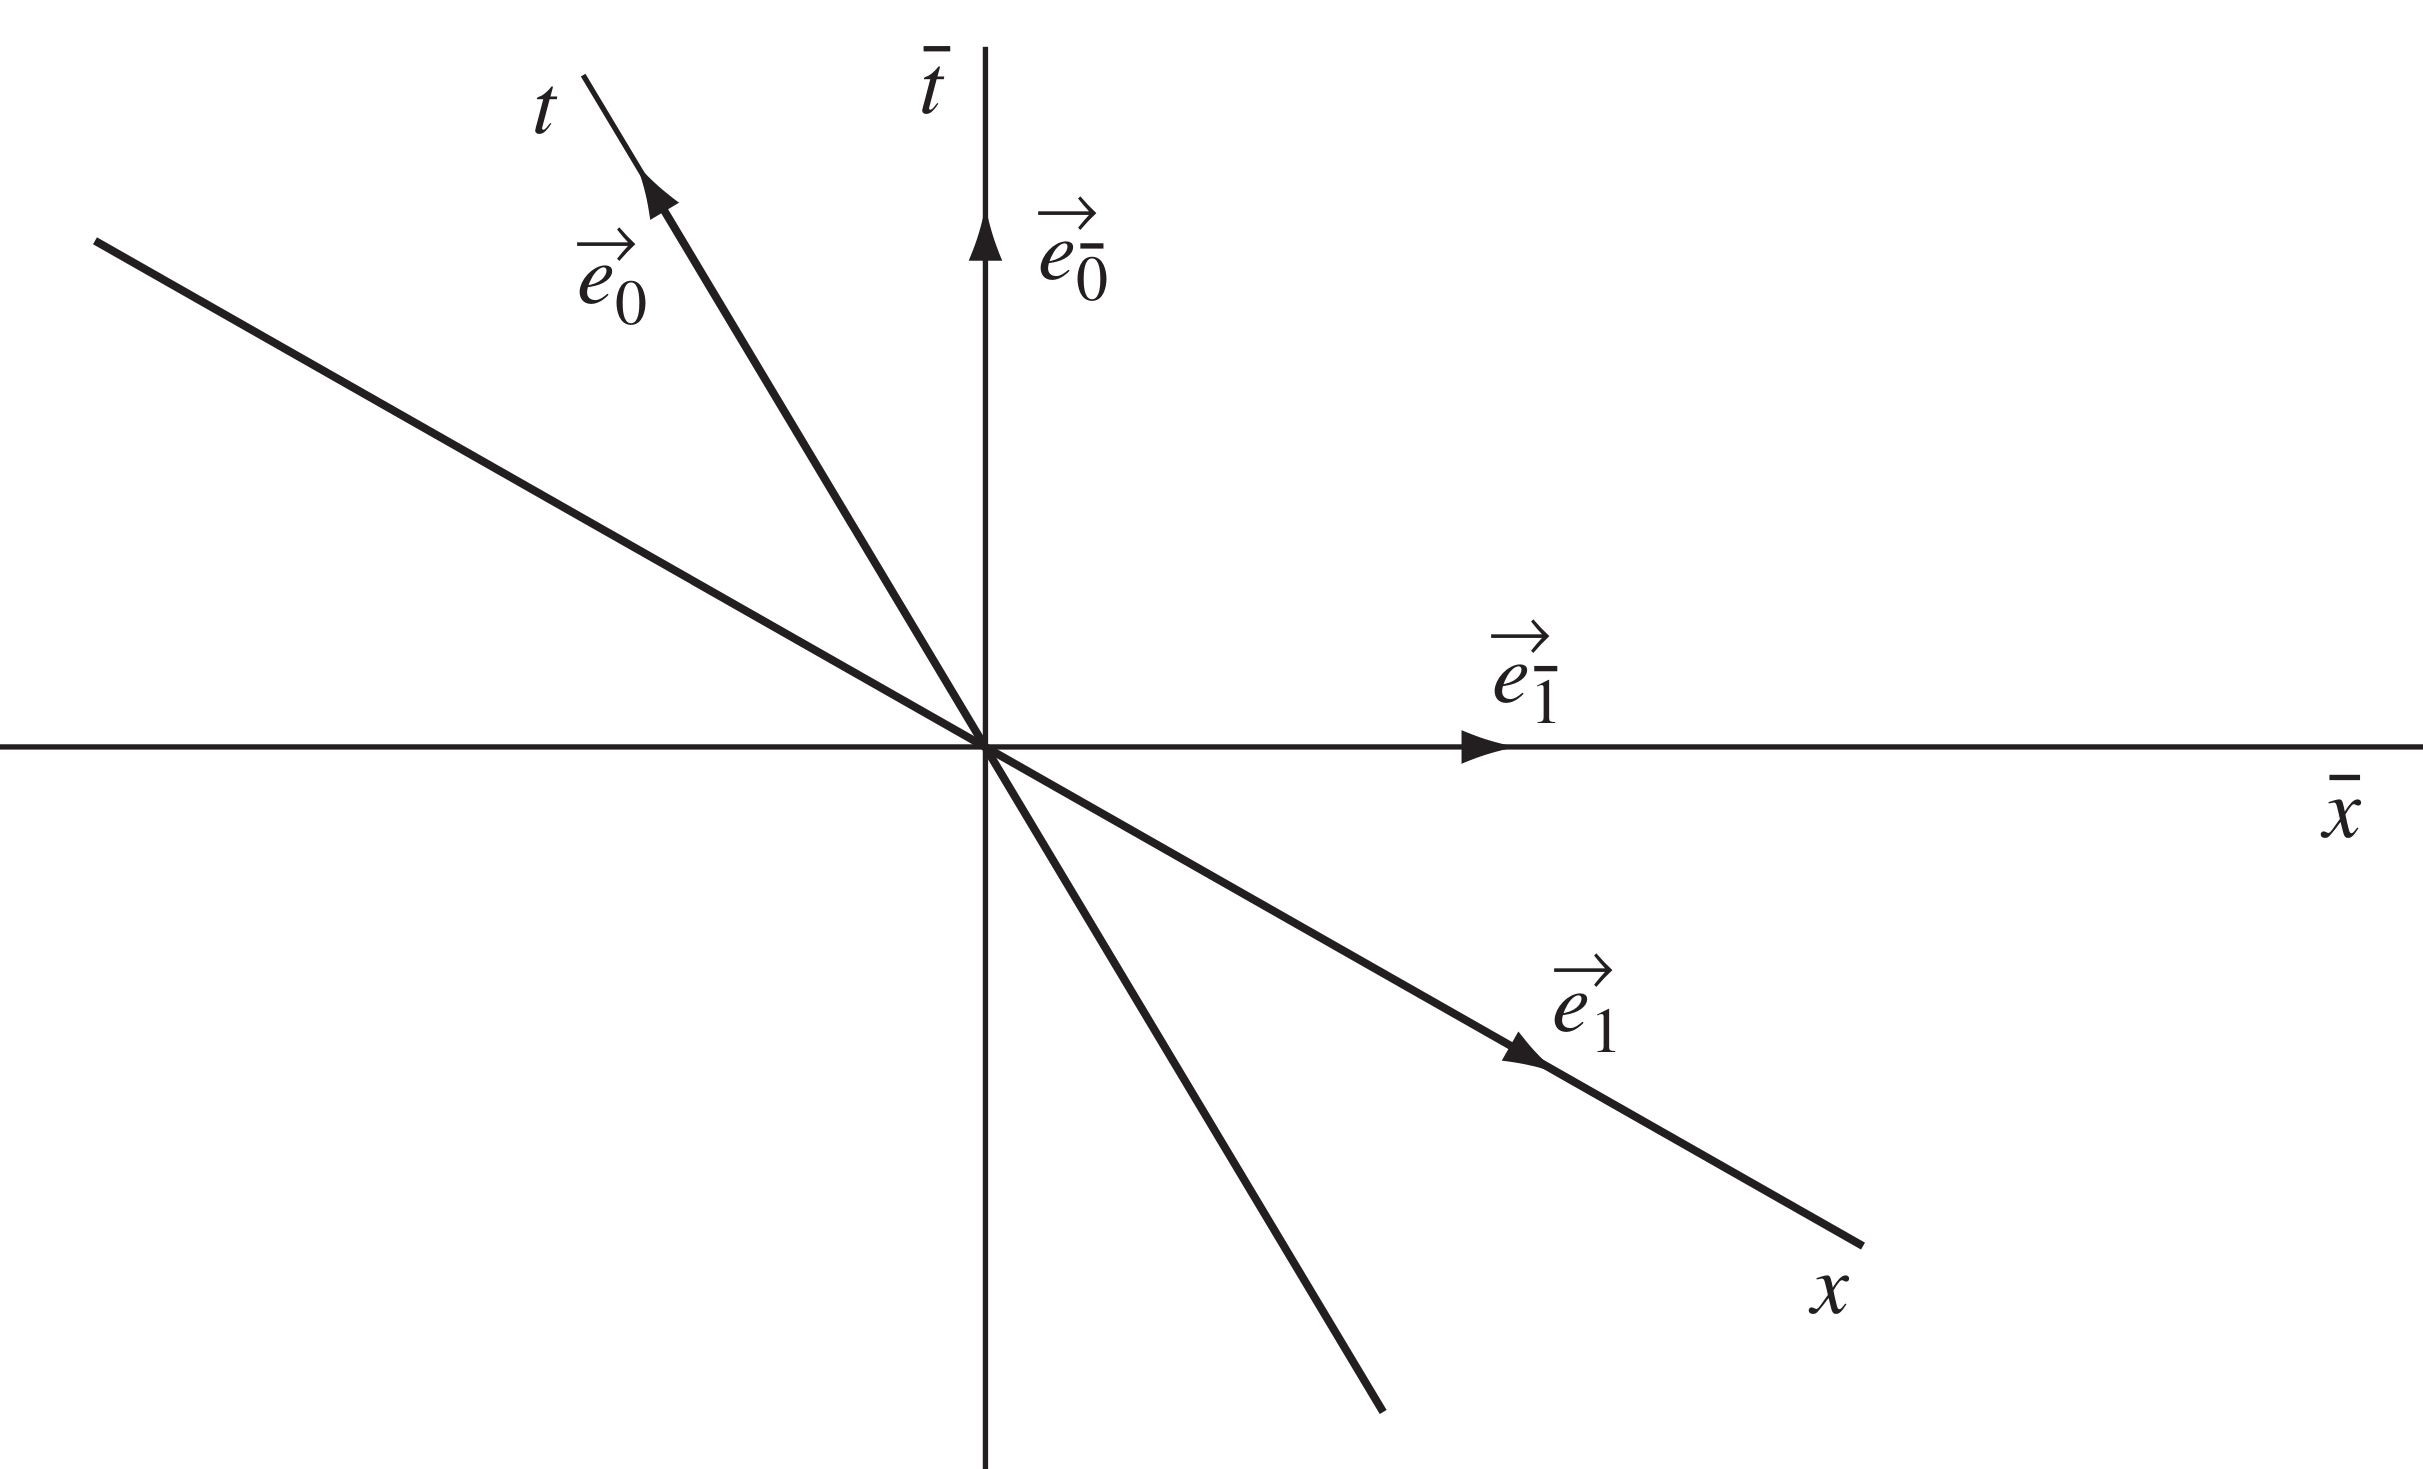
\includegraphics[width=0.7\textwidth]{fig2.1.png}
    \figcaption{\textit{ 在$\MObar$系中画出$\MO$系和$\MObar$系的基向量。 }}
    \label{fig2.1}
}



\subsection*{逆变换}
洛伦兹变换$\Lambda\indices{^{\bar{\beta}}_\alpha}$只依赖于两个坐标系之间的相对速度,下面将这种依赖关系写明:
\[
    \Lambda\indices{^{\bar{\beta}}_\alpha} = \Lambda\indices{^{\bar{\beta}}_\alpha} (\bm{v}).
\]
于是
\begin{equation}
    \Ve_\alpha = \Lambda\indices{^{\bar{\beta}}_\alpha} (\bm{v})\, \Ve_{\bar{\beta}}.
\label{equ2.14}
\end{equation}
如果$\MO$的基向量是通过$\MObar$的基向量经过速度$\bm{v}$对应的Lorentz变换得到的,那么逆变换必然是$(-\bm{v})$对应的,即:
\begin{equation}
    \Ve_{\bar{\mu}} = \Lambda\indices{^\nu_{\bar{\mu}}}(-\bm{v}) \, \Ve_\nu.
\label{equ2.15}
\end{equation}
上式采用新的$\bar{\mu}, \nu$以避免与上上式混淆,带bar的指标仍然是指$\MObar$系。矩阵$[\Lambda\indices{^\nu_{\bar{\mu}}}]$是矩阵$[\Lambda\indices{^{\bar{\beta}}_\alpha}]$将$\bm{v}$替换成$-\bm{v}$得到的。指标上的bar只是用来\textbf{标记}观测者:变换矩阵$[\Lambda]$相应的速度($\bm{v}$或者$-\bm{v}$)\textbf{总是}\textit{上标对应的坐标系}相对于\textit{下标对应的坐标系}的速度。这在\eqref{equ2.14}和\eqref{equ2.15}式特别清楚,$\bm{v}$是$\MObar$系(\eqref{equ2.14})式的上标坐标系)相对于$\MO$系的速度;而$-\bm{v}$是$\MO$系(\eqref{equ2.15}式的上标坐标系)相对于$\MObar$系的速度。本章习题11帮助读者进一步理解这一点。

\eqref{equ2.15}式可以写为
\[
    \Ve_{\bar{\beta}} = \Lambda\indices{^\nu_{\bar{\beta}}}(-\bm{v}) \, \Ve_\nu.
\]
上式只是把$\bar{\mu}$替换成了$\bar{\beta}$,方程的含义没有任何改变,同样是$\bar{\beta}$的四个值对应四个方程。上式带入$\Ve_\alpha$的表达式\eqref{equ2.14}式中:
\begin{equation}
    \Ve_\alpha = \Lambda\indices{^{\bar{\beta}}_\alpha}(\bm{v}) \, \Ve_{\bar{\beta}} = \Lambda\indices{^{\bar{\beta}}_\alpha}(\bm{v}) \Lambda\indices{^\nu_{\bar{\beta}}}(-\bm{v}) \, \Ve_\nu.
\label{equ2.16}
\end{equation}
上式只出现了$\MO$的基向量。因此它必然是对\textbf{所有}$\bm{v}$成立的恒等式。等式右侧含有两个求和,对$\bar{\beta}$和对$\nu$的。先计算对$\bar{\beta}$的求和,则等号右侧就是$\{ \Ve_\nu \}$的线性组合,每个$\Ve_\nu$对应的线性系数为:
\begin{equation}
    \sum_{\bar{\beta}} \Lambda\indices{^{\bar{\beta}}_\alpha}(\bm{v}) \, \Lambda\indices{^\nu_{\bar{\beta}}} (-\bm{v}).
\label{equ2.17}
\end{equation}
考虑\eqref{equ2.16}式中的某个固定的$\alpha$,等号成立意味着等号\textbf{右侧}的$\Ve_\alpha$的系数必须为1,而其余系数必须为0。用数学形式表示为
\[
    \Lambda\indices{^{\bar{\beta}}_\alpha}(\bm{v}) \, \Lambda\indices{^\nu_{\bar{\beta}}} (-\bm{v}) = \delta\indices{^\nu_\alpha},
\]
其中$\delta\indices{^\nu_\alpha}$是Kronecker delta符号,这样可以导出
\[
    \Ve_\alpha = \delta\indices{^\nu_\alpha} \Ve_\nu,
\]
它是个恒等式。

更换相乘顺序,将上面的关键公式写为
\begin{shaded}
\begin{equation}
    \Lambda\indices{^\nu_{\bar{\beta}}} (-\bm{v}) \, \Lambda\indices{^{\bar{\beta}}_\alpha}(\bm{v}) = \delta\indices{^\nu_\alpha}.
\label{equ2.18}
\end{equation}
\end{shaded}
上式意味着矩阵$[\Lambda\indices{^\nu_{\bar{\beta}}} (-\bm{v})]$和矩阵$[\Lambda\indices{^{\bar{\beta}}_\alpha}(\bm{v})]$\textbf{互逆},因为对$\bar{\beta}$的求和意味着两个矩阵相乘。矩阵$(\delta\indices{^\nu_\alpha})$就是单位矩阵。

向量分量的变换式
\[
    A^{\bar{\beta}} = \Lambda\indices{^{\bar{\beta}}_\alpha}(\bm{v}) \, A^\alpha,
\]
也有相应的逆形式。等号两侧乘以$\Lambda\indices{^\nu_{\bar{\beta}}} (-\bm{v})$,对$\bar{\beta}$求和:
\begin{align*}
    \Lambda\indices{^\nu_{\bar{\beta}}} (-\bm{v})  \, A^{\bar{\beta}} &= \Lambda\indices{^\nu_{\bar{\beta}}} (-\bm{v}) \, \Lambda\indices{^{\bar{\beta}}_\alpha}(\bm{v}) \, A^\alpha \\
    &= \delta\indices{^\nu_\alpha} A^\alpha \\
    &= A^\nu.
\end{align*}
这意味着$\vec{A}$在$\MO$系的分量等于$\MObar$系的分量经过速度$-\bm{v}$对应的Lorentz变换得到,我们得到了正确结论。

上述内容与读者熟悉的欧几里得空间中的向量代数类似,只是这里采用了新的指标记号,这种记号在本书其余的部分大用特用。读者应该掌握上述内容的几何意义以及代数依据。



\section{四维速度}
\label{sec2.3}
世界线的四维速度(four-velocity, 简称四速)是一种十分重要的向量。伽利略的三维几何中,速度是与粒子运动轨迹相切的向量。四维几何的四维速度$\vec{U}$定义为与粒子世界线相切的、在粒子的参考系中长度为单位时间的向量。先考虑最简单的匀速直线运动粒子,在与粒子相对静止的惯性系中,根据定义,四维速度向量的方向与时间轴平行、长度为单位时间,这意味着四维速度就等于该系的基向量$\vec{e}_0$。于是,匀速直线运动粒子的四维速度定义为该粒子静止惯性系的基向量$\vec{e}_0$. “四维速度”名字的来历是$\vec{U}$的空间分量与通常所说的粒子的三维速度$\bm{p}$关系密切,参见下面的例子与\eqref{equ2.21}式。


\textit{变速运动的粒子}不存在始终在其中静止的惯性系。然而,\textit{仍然存在着}与粒子瞬时静止的惯性系——它的速度在一瞬间与粒子速度相同(共动参考系),不过在下一时刻就不再是共动的了。这个参考系称为\textit{瞬时共动参考系 (momentarily comoving reference frame,} \textbf{\ MCRF} \textit{)},这个概念极其重要。(实际上,一个粒子在某一特定事件点有无数个MCRF;它们的速度相同,而空间坐标轴相差旋转变换。不过这通常不重要,取哪个空间轴取向的MCRF都行)变速运动粒子(在某一事件点)的四速\textit{定义为}在该事件点的MCRF的基向量$\vec{e}_0$. 该向量与(弯曲的)粒子世界线相切。图\ref{fig2.2}中,粒子在事件$\mathscr{A}$的MCRF是$\MObar$系,图中画出了基向量,$\vec{e}_{\bar{0}}$就是粒子在$\mathscr{A}$点的四速$\vec{U}$.

{
    \centering
    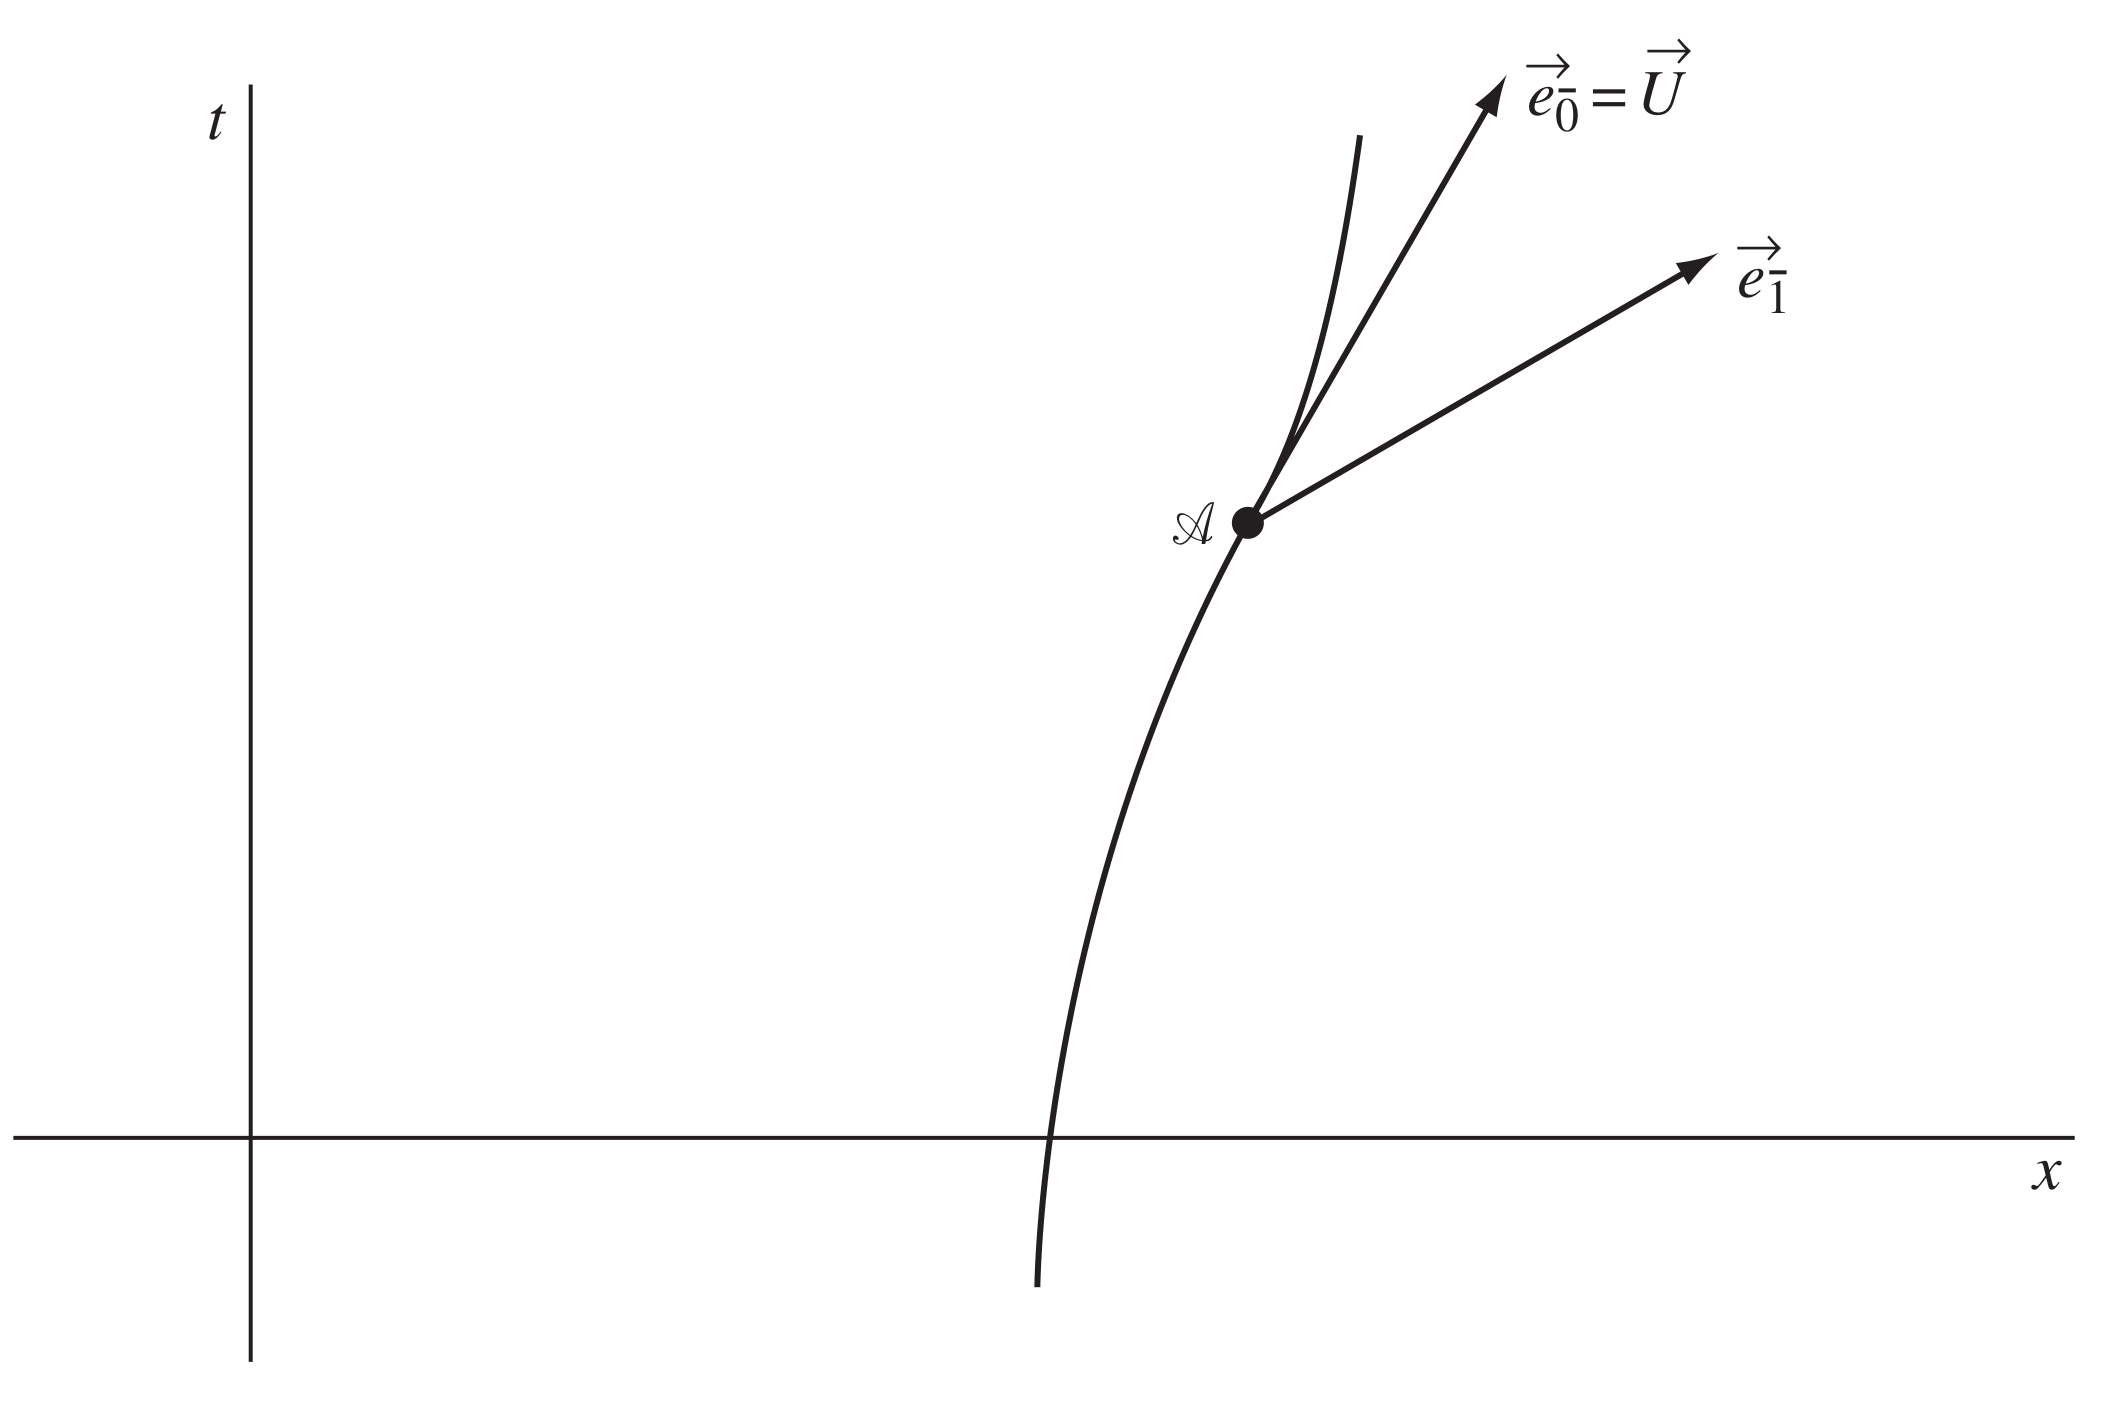
\includegraphics[width=0.7\textwidth]{fig2.2.png}
    \figcaption{\textit{粒子世界线在$\mathscr{A}$点的四维速度与MCRF基向量}}
    \label{fig2.2}
}


\section{四维动量}
\label{sec2.4}
四维动量$\vec{p}$定义为
\begin{shaded}
\begin{equation}
    \vec{p} = m \vec{U},
\label{equ2.19}
\end{equation}
\end{shaded}
其中$m$是粒子的\textit{静止质量 (rest mass,简称静质量)},也就是在粒子静止的坐标系中测得的粒子质量。四动量在任一惯性系$\MO$中的分量记作
\begin{equation}
    \vec{p} \xrightarrow[\MO]{ } (E, p^1, p^2, p^3).
\label{equ2.20}
\end{equation}
分量$p^0$记作$E$,称为粒子在坐标系$\MO$中的\textit{能量 (energy)}。其余分量称为四动量的空间分量$p^i$.

\subsection*{例子}
静质量为$m$的粒子在坐标系$\MO$中沿$x$轴方向运动,速度为$\bm{v}$,粒子四速、四动量在$\MO$系的分量是什么?粒子在其中静止的坐标系记作$\MObar$,该系的时间基向量为$\vec{e}_{\bar{0}}$。根据四速与四动量的定义有
\begin{equation}
\begin{split}
    \vec{U} &= \vec{e}_{\bar{0}}, & \quad \vec{p} &= m\vec{U}, \\
    U^\alpha &= \Lambda\indices{^\alpha_{\bar{\beta}}} ( \vec{e}_{\bar{0}} )^{\bar{\beta}} = \Lambda\indices{^\alpha_{\bar{0}}}, \quad & p^\alpha &= m \Lambda\indices{^\alpha_{\bar{0}}}.
\end{split}
\label{equ2.21}
\end{equation}
由此可得
\begin{align*}
    U^0 &= (1 - v^2)^{-1/2}, \quad & p^0 &= m(1 - v^2)^{-1/2}, \\
    U^1 &= v (1 - v^2)^{-1/2}, \quad & p^1 &= mv (1 - v^2)^{-1/2}, \\
    U^2 &= 0, \quad & p^2 &= 0, \\
    U^3 &= 0, \quad & p^3 &= 0.
\end{align*}
对于很小的$v$,$\vec{U}$的空间分量近似为$(v, 0, 0)$,$\vec{p}$的空间分量为$(mv, 0, 0)$,从这就能看出它们的名字——四维速度、四维动量——的合理性。还是对于很小的$v$,能量近似为:
\begin{equation*}
    E := p^0 = m (1 - v^2)^{-1/2} \approx m + \frac{1}{2} m v^2.
\end{equation*}
它等于静质能(rest-mass energy)与(伽利略形式的)动能之和。

\subsection*{四维动量守恒}
伽利略力学中,粒子的碰撞过程遵从能量、动量守恒定律。因为$\vec{p}$的分量在非相对论极限下退化为伽利略形式的能量、动量,因此很自然地假设在相对论情形下,四维向量$\vec{p}$也守恒。也就是说,几个粒子发生相互作用,粒子的总动量:
\begin{equation}
    \vec{p} := \sum_{\text{所有粒子,编号为}(i)} \vec{p}_{(i)},
\label{equ2.22}
\end{equation}
在碰撞过程的前后不变。($\vec{p}_{(i)}$是第$i$个粒子的动量)

四维动量守恒定律实际上是个额外\textit{假设},因为我们只知道它的非相对论极限是正确的。不过就像SR的两条基本假设那样,四动量守恒经历了丰富的实验验证。至少它预言了能量守恒定律必须包括静质能:静质量可以消灭、相应的能量可以转化为动能从而化为热能。这个预言每天都在被核电站所验证。

上面四动量守恒的陈述中掩藏了很重要的一点:一次碰撞“之前”与“之后”的含义是什么?假设不同的粒子发生了两次碰撞,这两个事件的间隔是类空的,如下图。要将同一时刻的四动量相加,应该沿着等$t$时刻还是等$\bar{t}$时刻?如图\ref{fig2.3}所示,$\MO$系的测量结果为:事件$\mathscr{A}$发生在$t = 0$之前,事件$\mathscr{B}$在之后,因此$t = 0$时刻的总动量等于$\mathscr{A}$之后加上$\mathscr{B}$之前的动量。而在$\MObar$系中,事件$\mathscr{A}, \mathscr{B}$同时发生于时刻$\bar{t} = 0$之前,因此$\bar{t} = 0$时刻的总动量等于事件$\mathscr{A}, \mathscr{B}$之后的动量之和。 甚至还可以找到一个坐标系,在其中事件$\mathscr{B}$比$\mathscr{A}$发生的\textit{更早},and the adding-up may be the reverse of $\MO$'s. 

{
    \centering
    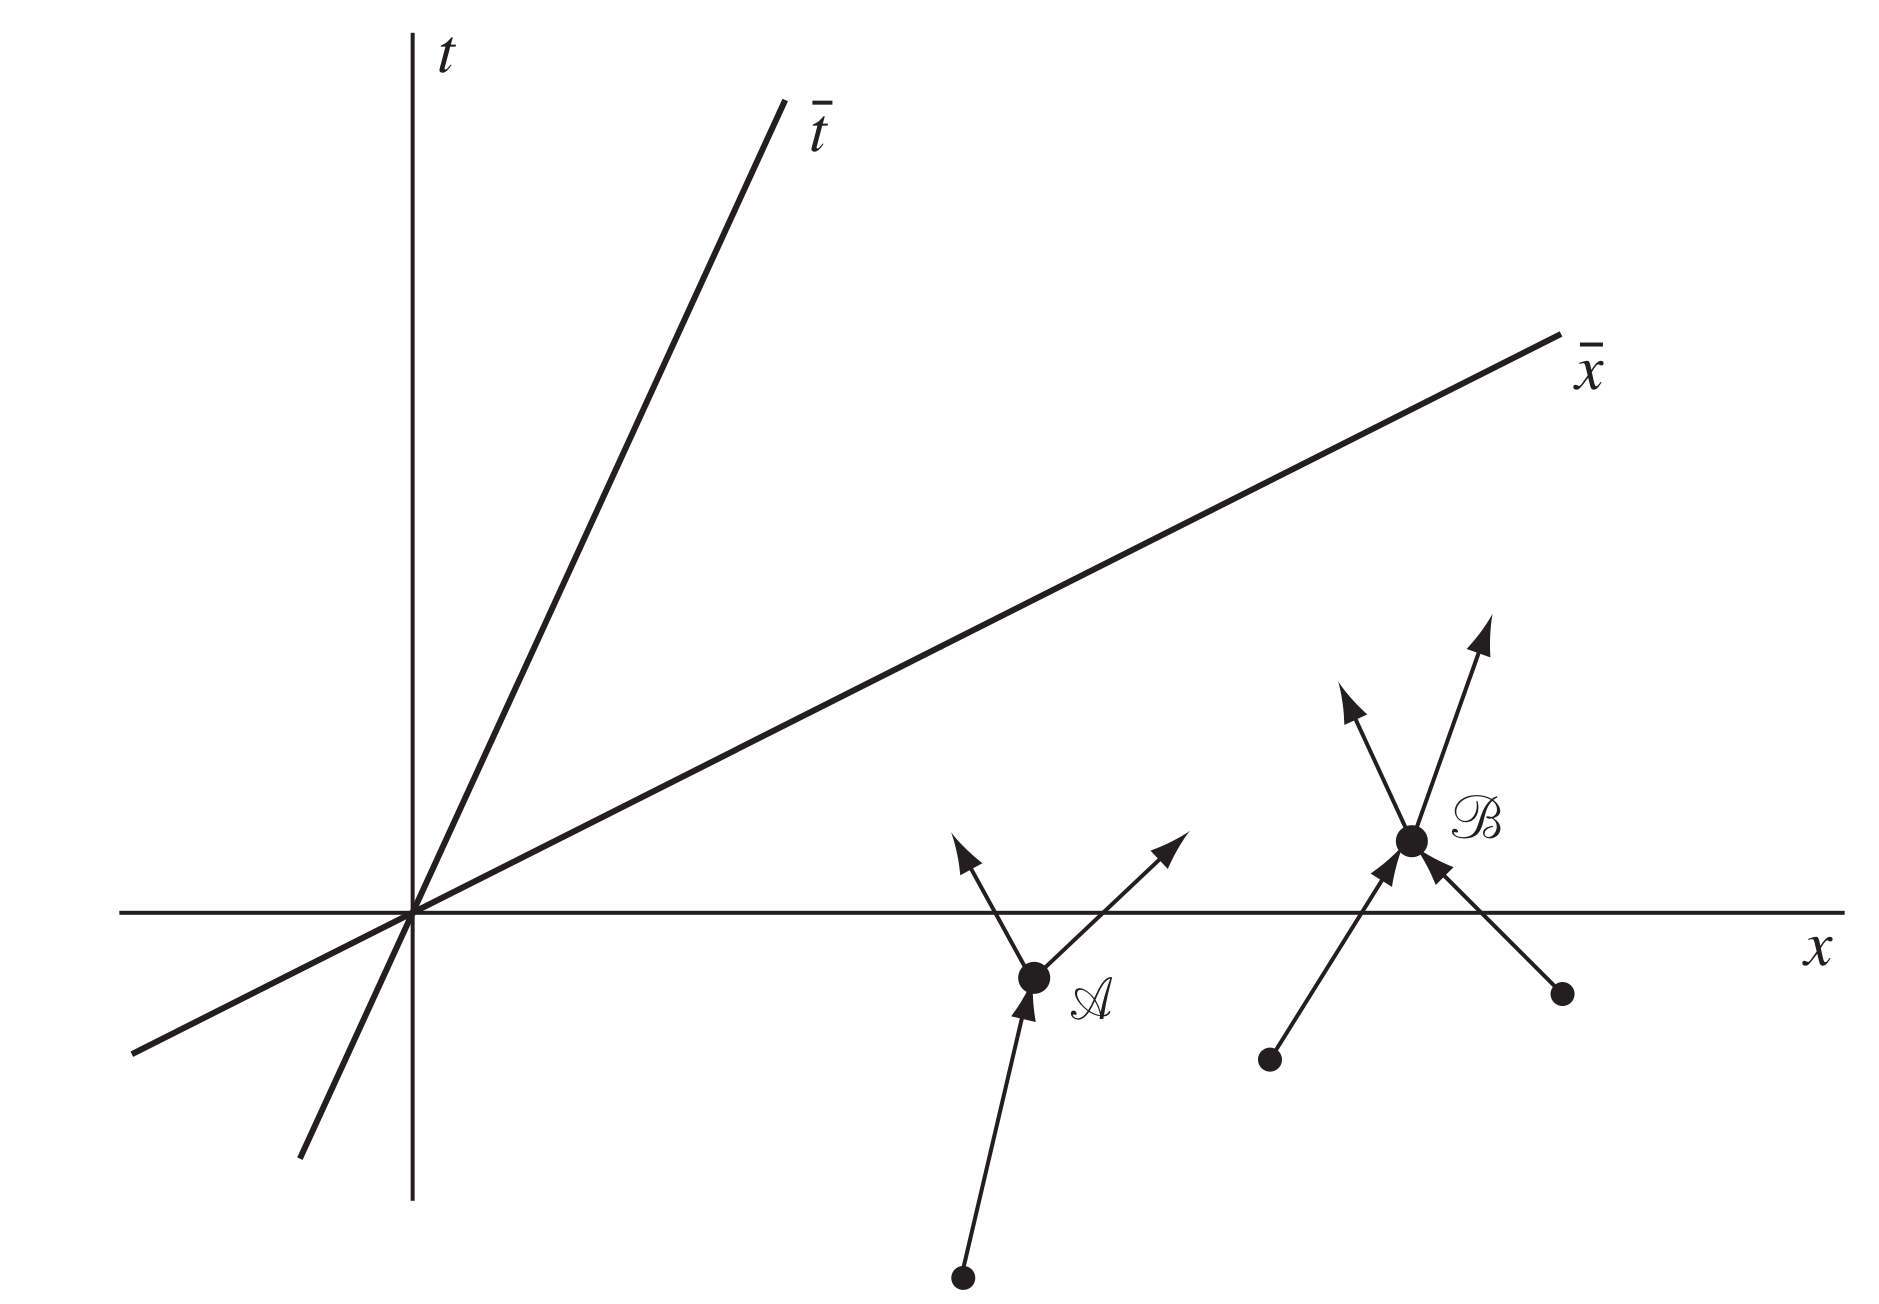
\includegraphics[width=0.7\textwidth]{fig2.3.png}
    \figcaption{\textit{当考虑几个碰撞过程时,组成某一时刻的总动量的各个四动量取决于坐标系,但总的四维动量是在所有坐标系中相同的四维向量;它的分量在坐标系之间的变换规律服从Lorentz变换。}}
    \label{fig2.3}
}

这实际上没问题。既然每个碰撞过程都服从动量守恒,那么事件$\mathscr{A}$之后与之前的动量和相等,事件$\mathscr{B}$也一样。因此\textit{每个}惯性观者都得到相同的总的四动量$\vec{p}$。(它的分量随坐标系的不同而不同,但是它是同一个向量。) 有一点很重要:\textit{任意}观者可以定义他自己的等时线(这实际上是等时的三维空间,称之为四维时空中等时的\textit{超平面}),把那个时刻的所有动量相加,得到的向量与其他任何观者的结果都相同。理解这一点十分重要,因为这种守恒律会在之后再次出现。

\subsection*{质心 (CM) 系}
质心系(center of momentum frame, CM)是总动量的空间分量在其中为零的惯性系:
\begin{equation}
    \sum_i \vec{p}_{(i)} \xrightarrow[\text{CM}]{ } (E_{\text{TOTAL}}, 0, 0, 0).
\label{equ2.23}
\end{equation}
与MCRF同理,任意相对于CM系静止的坐标系也是CM系。

\section{标量积}
\label{sec2.5}

\subsection*{四维向量的模}
类比间隔的定义,四维向量$\vec{A}$的\textit{模 (magnitude)}定义为
\begin{equation}
    \vec{A}^2 = -(A^0)^2 + (A^1)^2 + (A^2)^2 + (A^3)^2.
\label{equ2.24}
\end{equation}
根据向量分量的\textit{定义},向量分量在坐标变换下与$(\Delta t, \Delta x, \Delta y, \Delta z)$的变换规律相同,服从Lorentz变换,这就\textit{保证了}
\begin{equation}
    -(A^0)^2 + (A^1)^2 + (A^2)^2 + (A^3)^2 = -(A^{\bar{0}})^2 + (A^{\bar{1}})^2 + (A^{\bar{2}})^2 + (A^{\bar{3}})^2.
\label{equ2.25}
\end{equation}
向量的模就定义成这样的不依赖于坐标系的量,即Lorentz变换下的标量 (scalar)。

向量模不一定是正数。我们把向量按照间隔那样进行分类:
\begin{itemize}
    \item 如果$\vec{A}^2$是正数,则称$\vec{A}$是\textit{类空 (spacelike)}向量;
    \item 如果$\vec{A}^2$等于零,则称$\vec{A}$是\textit{null}向量\footnote{通译为“零向量”,然而这个名字给人一种\sout{钦定的}所有分量都为零的感觉,事实上并非如此(例如向量$(1, 1, 0, 0)$的模$\big( -(1)^2 + 1^2 \big) = 0$. 因此我们不采用“零向量”的译法,暂时称呼它为“null 向量”。};
    \item 如果$\vec{A}^2$是负数,则称$\vec{A}$是\textit{类时 (timelike)}向量。
\end{itemize}
这样,空间中的向量的模是正数,就像欧几里得空间的情况那样。必须注意,null向量\textit{不同于}zero向量。也就是说,null向量满足$\vec{A}^2 = 0$,但它的所有$A^\alpha$不一定都为零;而zero向量的所有分量都是零。只有在$\vec{A}^2$均为正定(positive-definite)的空间中,$\vec{A}^2 = 0$才意味着$\forall\, \alpha, A^\alpha = 0$.

\subsection*{两个向量的标量积}
向量$\vec{A}, \vec{B}$(在某个惯性系$\MO$)的标量积 (scalar product)定义为
\begin{shaded}
\begin{equation}
    \vec{A} \cdot \vec{B} = -A^0 B^0 + A^1 B^1 + A^2 B^2 + A^3 B^3.
\label{equ2.26}
\end{equation}
\end{shaded}
下面来证明这个标量积在其它惯性系也是同样的值。

首先注意到$\vec{A} \cdot \vec{A}$就是$\vec{A}^2$,我们已经知道后者是个坐标变换下的不变量。因此$(\vec{A} + \vec{B}) \cdot ( \vec{A} + \vec{B} )$,即$\vec{A} + \vec{B}$的模,也是不变量。根据\eqref{equ2.24}和\eqref{equ2.26}式可得
\begin{equation*}
    (\vec{A} + \vec{B}) \cdot ( \vec{A} + \vec{B} ) = \vec{A}^2 + \vec{B}^2 + 2 \vec{A} \cdot \vec{B}.
\end{equation*}
因为等号左侧的项以及右侧的前两项在所有坐标系中相等,因此最后一项也在所有坐标系中相等。这就证明了向量积是坐标系不变量。

如果$\vec{A} \cdot \vec{B} = 0$,则称向量$\vec{A}$与$\vec{B}$\textit{垂直 (orthogonal)}。标量积定义中的负号意味着相互垂直的两个向量不一定非得在时空图中成直角(见下文的例子)。一种极端情况是null向量,它与\textit{自身}垂直!这种现象在标量积是正定的空间中不会出现。

\subsection*{例1}
$\MO$系的基向量满足:
\begin{align*}
    \vec{e}_0 \cdot \vec{e}_0 &= -1, \\
    \vec{e}_1 \cdot \vec{e}_1 &= \vec{e}_2 \cdot \vec{e}_2 = \vec{e}_3 \cdot \vec{e}_3 = +1, \\
    \vec{e}_\alpha \cdot \vec{e}_\beta &= 0, \quad \text{如果} \ \alpha \neq \beta.
\end{align*}
因此它们组成了一组相互正交的向量四元组:一组\textit{规范正交基},这意味着这组基的所有基向量\textit{相互正交}并且\textit{归一化}——具有单位模. (类空向量的“单位模”意味着模为$-1$.)上式可以总结为
\begin{shaded}
\begin{equation}
    \vec{e}_\alpha \cdot \vec{e}_\beta = \eta_{\alpha \beta},
\label{equ2.27}
\end{equation}
\end{shaded}
其中$\eta_{\alpha \beta}$和Kronecker\ $\delta$符号有点像——当$\alpha \neq \beta$时$\eta_{\alpha \beta} = 0$,但有所不同:$\eta_{00} = -1, \eta_{11} = \eta_{22} = \eta_{33} = +1$. 后面会看到$\eta_{\alpha \beta}$的地位极其重要:它是度规张量。不过现在把它当作Kronecker\ $\delta$的推广就好了。

\subsection*{例2}
$\MObar$系的基向量也满足
\begin{equation*}
    \vec{e}_{\bar{\alpha}} \cdot \vec{e}_{\bar{\beta}} = \eta_{\bar{\alpha} \bar{\beta}},
\end{equation*}
因此$\vec{e}_{\bar{0}} \cdot \vec{e}_{\bar{1}} = 0$. 考虑图\ref{fig2.4}中的时空图:图中的$\vec{e}_{\bar{0}}, \vec{e}_{\bar{1}}$看起来不垂直。然而它们的标量积等于零。如果两个向量与$45^\circ$倾斜的直线(光的世界线)的夹角相等,那么这两个向量垂直。因此,与光的世界线相切的向量与自身垂直。这是SR中不能用欧几里得空间类比的又一个概念。

{
    \centering
    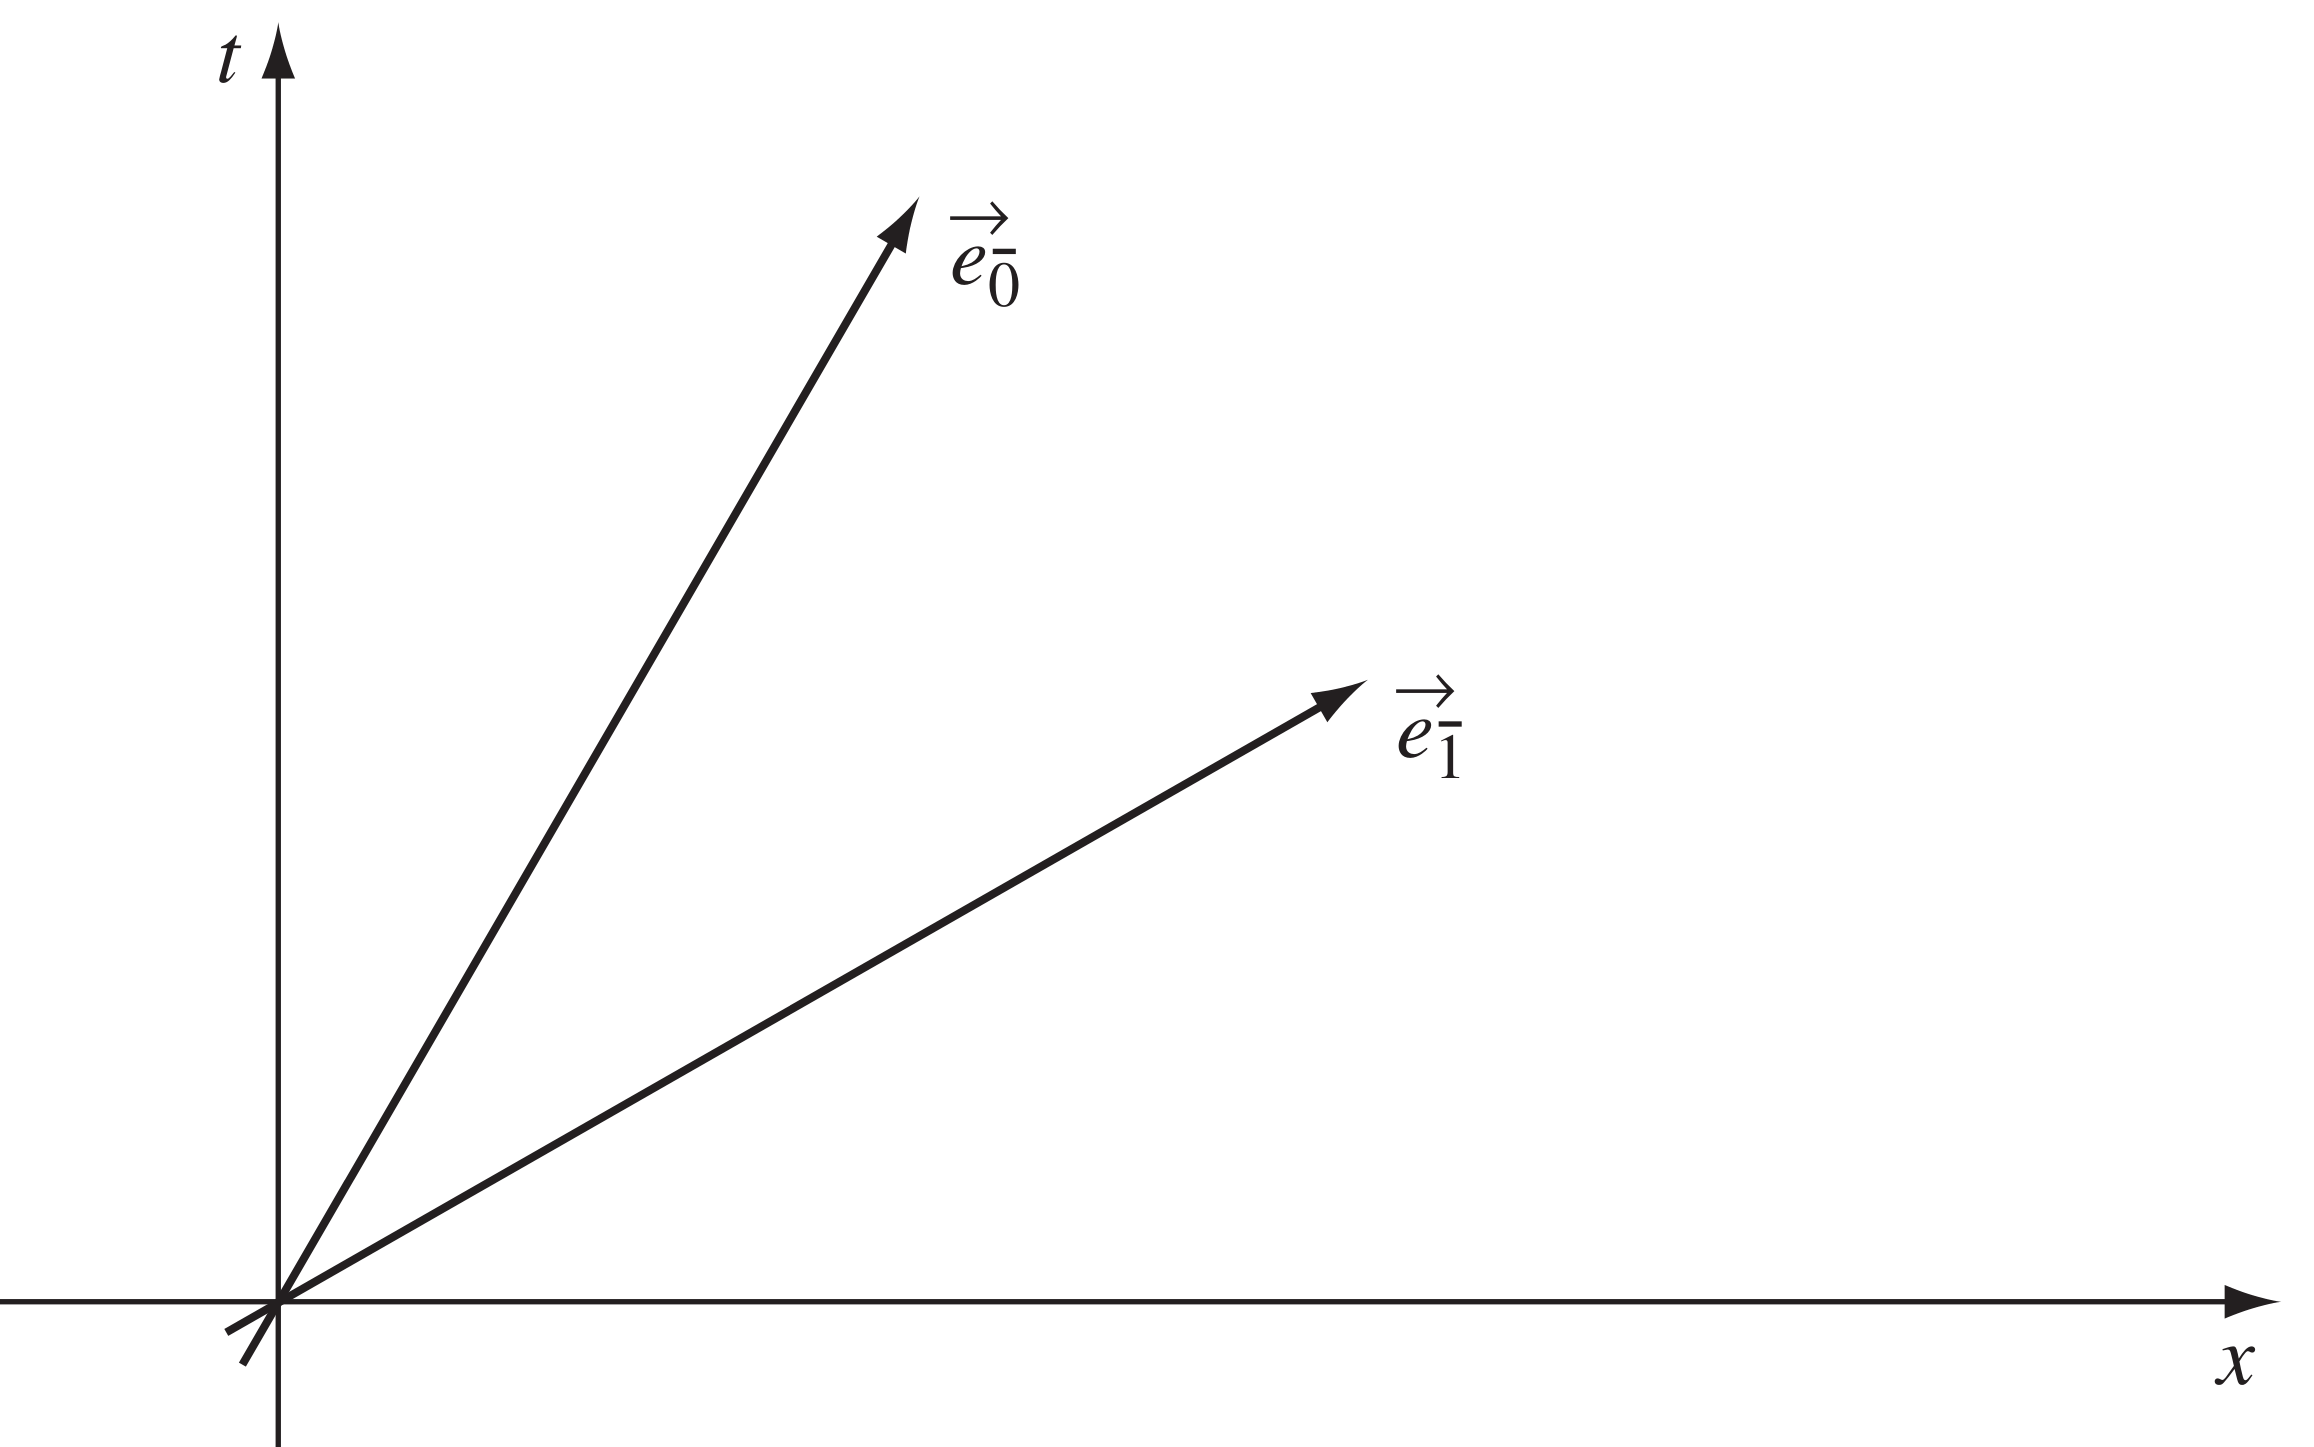
\includegraphics[width=0.5\textwidth]{fig2.4.png}
    \figcaption{\textit{在$\MO$系之下,$\MObar$系的基向量(用欧几里得空间的眼光)看起来并不“垂直”,但是它们在Minkowski时空的向量积定义下却是正交的。}}
    \label{fig2.4}
}

\subsection*{例3}
粒子的四维速度$\vec{U}$就是粒子MCRF的基向量,因此根据\eqref{equ2.27}式可得
\begin{equation}
    \vec{U} \cdot \vec{U} = -1.
\label{equ2.28}
\end{equation}

\section{应用}
\label{sec2.6}

\subsection*{四速与四加速的导数形式}
设粒子进行了无穷小位移$\rd \vec{x}$,$\rd \vec{x}$在$\MO$系的分量是$(\rd t, \rd x, \rd y, \rd z)$。根据\eqref{equ2.24}式,无穷小位移的模等于$-\rd t^2 + \rd x^2 + \rd y^2 + \rd z^2$. 与\eqref{equ1.1}式进行比较,可以发现这就是间隔$\rd s^2$:
\begin{equation}
    \rd s^2 = \rd \vec{x} \cdot \rd \vec{x}.
\label{equ2.29}
\end{equation}
因为粒子世界线是类时的,因此上式各项为负数。这启示我们(方程\eqref{equ1.9})定义\textbf{固有时 (proper time)} $\rd \tau$为
\begin{equation}
    (\rd \tau)^2 = -\rd \vec{x} \cdot \rd \vec{x}.
\label{equ2.30}
\end{equation}

{
    \centering
    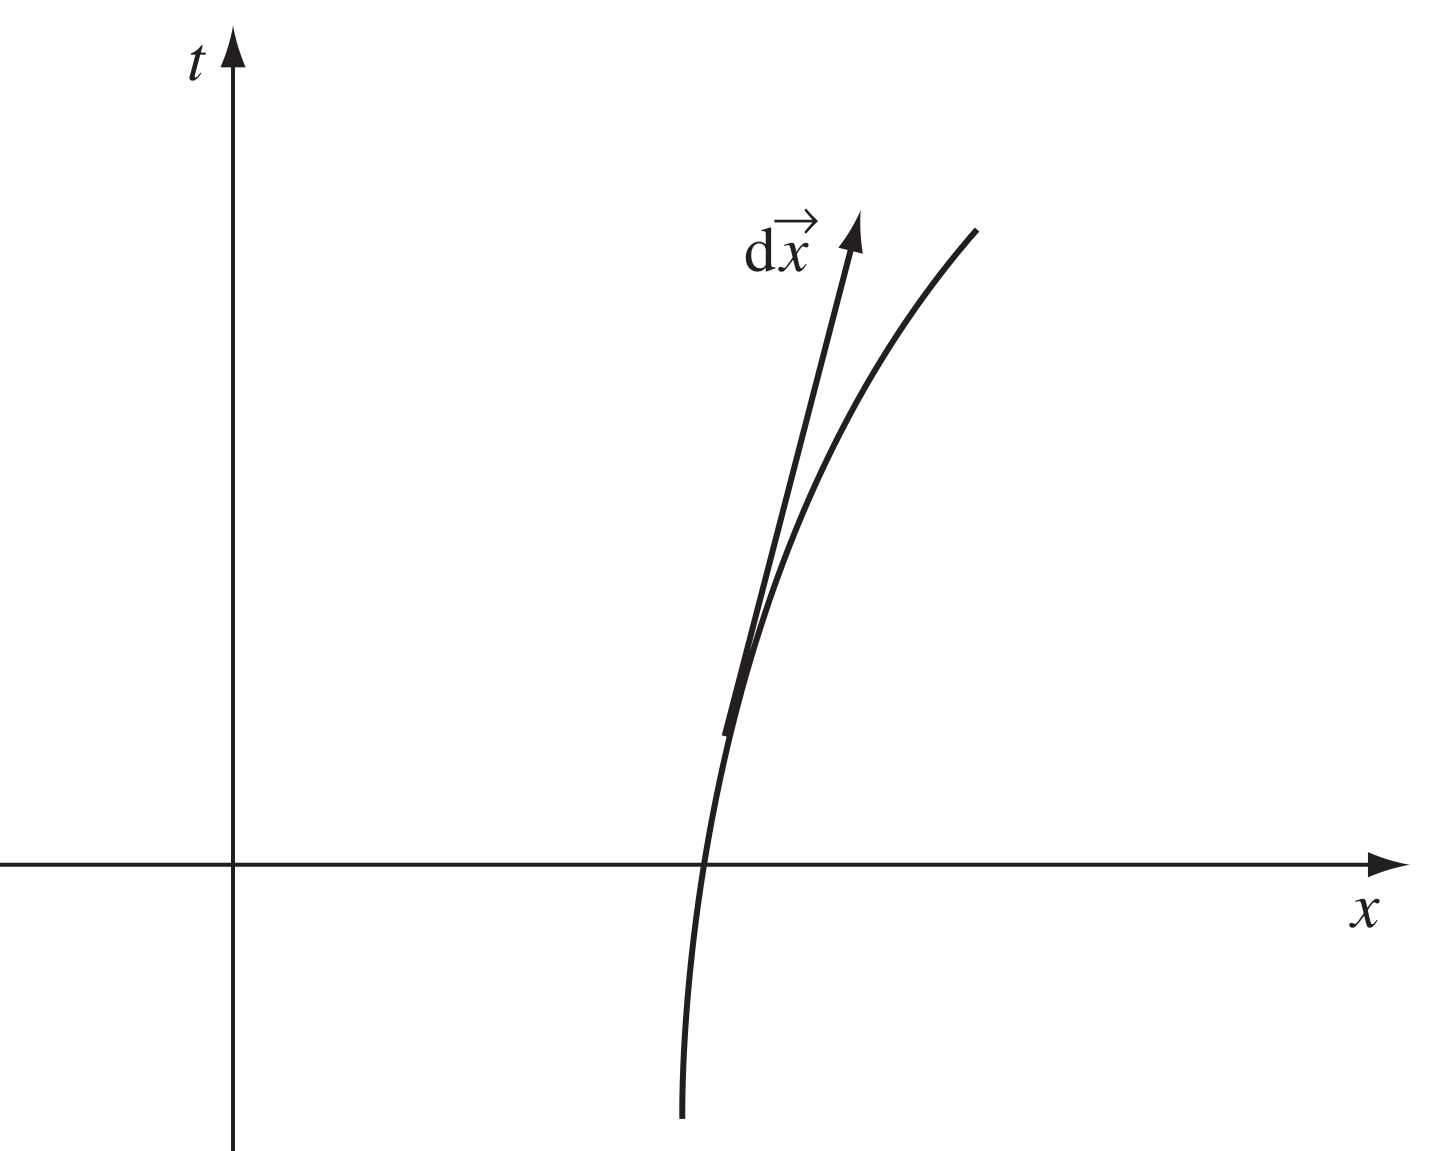
\includegraphics[width=0.6\textwidth]{fig2.5.png}
    \figcaption{\textit{与粒子世界线相切的无穷小位移向量$\rd \vec{x}$.}}
    \label{fig2.5}
}

下面来考虑向量$\rd \vec{x} / \rd \tau$,其中$\rd \tau$等于方程\eqref{equ2.30}的平方根(如图\ref{fig2.5})。这个向量与世界线相切,因为它是$\rd \vec{x}$的倍数。它的模等于
\begin{equation*}
    \frac{\rd \vec{x}}{\rd \tau} \cdot \frac{\rd \vec{x}}{\rd \tau} = \frac{\rd \vec{x} \cdot \rd \vec{x}}{(\rd \tau)^2} = -1.
\end{equation*}
因此它是与世界线相切的、单位模长的类时向量。在MCRF中:
\[
    \rd \vec{x} \xrightarrow[\text{MCRF}, \rd \tau = \rd t]{ } (\rd t, 0, 0, 0).
\]
因此
\[
    \frac{\rd \vec{x}}{\rd \tau} \xrightarrow[\text{MCRF}]{ } (1, 0, 0, 0),
\]
从而有
\[
    \frac{\rd \vec{x}}{\rd \tau} = (\vec{e}_0)_{\text{MCRF}}.
\]
上式右侧就是四维速度的\textit{定义}。由此可得如下的常用表达式:
\begin{shaded}
\begin{equation}
    \vec{U} = \frac{\rd \vec{x}}{\rd \tau}.
\label{equ2.31}
\end{equation}
\end{shaded}

进一步再考虑
\[
    \frac{\rd \vec{U}}{\rd \tau} = \frac{\rd^2 \vec{x}}{\rd \tau^2},
\]
这有一种四维加速度的感觉。我们对方程\eqref{equ2.28}式进行微分,并利用\eqref{equ2.26}式可得
\[
    \frac{\rd}{\rd \tau} (\vec{U} \cdot \vec{U}) = 2 \vec{U} \cdot \frac{\rd \vec{U}}{\rd \tau}.
\]
因为$\vec{U} \cdot \vec{U} = -1$,是个常数,因此
\[
    \vec{U} \cdot \frac{\rd \vec{U}}{\rd \tau} = 0.
\]
由于在MCRF中,$\vec{U}$只有0分量,因此上式的正交性意味着
\[
    \frac{\rd \vec{U}}{\rd \tau} \xrightarrow[\text{MCRF}]{ } (0, a^1, a^2, a^3).
\]
这个向量定义为四维\textit{加速度}向量,记作$\vec{a}$:
\begin{shaded}
\begin{equation}
    \vec{a} = \frac{\rd \vec{U}}{\rd \tau}, \quad \vec{U} \cdot \vec{a} = 0.
\label{equ2.32}
\end{equation}
\end{shaded}
本章习题19说明了为啥叫它“加速度”。

\subsection*{能量与动量}
考虑一个动量为$\vec{p}$的粒子,
\begin{equation}
    \vec{p} \cdot \vec{p} = m^2 \vec{U} \cdot \vec{U} = -m^2.
\label{equ2.33}
\end{equation}
由于
\[
    \vec{p} \cdot \vec{p} = -E^2 + (p^1)^2 + (p^2)^2 + (p^3)^2.
\]
因此
\begin{equation}
    E^2 = m^2 + \sum_{i = 1}^3 (p^i)^2.
\label{equ2.34}
\end{equation}
这是粒子总能量的常用表达式。

某观测者以四速$\vec{U}_{\text{obs}}$运动,他在其中静止的坐标系记作$\MObar$,观者的四速可以不等于粒子四速。
\[
    \vec{p} \cdot \vec{U}_{\text{obs}} = \vec{p} \cdot \vec{e}_{\bar{0}},
\]
其中$\vec{e}_{\bar{0}}$是$\MObar$系的基向量,在该系中粒子四动量的分量为
\[
    \vec{p} \xrightarrow[\MObar]{ } (\bar{E}, p^{\bar{1}}, p^{\bar{2}}, p^{\bar{3}}).
\]
于是,根据\eqref{equ2.26}式可得:
\begin{shaded}
\begin{equation}
    -\vec{p} \cdot \vec{U}_{\text{obs}} = \bar{E}.
\label{equ2.35}
\end{equation}
\end{shaded}
这个结果超级重要。它表明,粒子相对于观测者的能量$\bar{E}$可以在任意坐标系中通过计算标量积$\vec{p} \cdot \vec{U}_{\text{obs}}$得到,这称为相对于观测者的能量的“坐标系无关”的表达式。它在大多数情形下都很有用。

\section{光子}
\label{sec2.7}
\subsection*{光子无四速}
光子在时空图的轨迹是null直线(即切向量都是null向量的直线),即,光子世界线轨迹满足
\begin{equation}
    \rd \vec{x} \cdot \rd \vec{x} = 0.
\label{equ2.36}
\end{equation}
因此$\rd \tau$为零。方程\eqref{equ2.31}表明\textit{光子四速不能定义}。导出该结论的另一种方式是注意到不存在光子在其中静止的坐标系(根据SR的第二个假设),因此光子没有MCRF。所以没有哪个坐标系的$\vec{e}_0$会与光子世界线相切。

注意,仍然可以找到与光子轨迹相切的向量(光子世界线轨迹为直线,它每一点的切向量相等):$\rd \vec{x}$就是一个。问题是找不到\text{单位模长}的切向量,因为所有切向量的模等于零。

\subsection*{四动量}
粒子的四动量\textit{不是}单位向量。粒子四动量在某个坐标系的分量是粒子在那个系中的能量、动量。如果光子在某坐标系中的能量为$E$,则在该系中$p^0 = E$。如果光子在该系中沿$x$轴方向运动,则$p^y = p^z = 0$,由于四动量必须与光子世界线平行,因此光子四动量必须是null向量,从而有$p^x = E$,这保证了
\begin{equation}
    \vec{p} \cdot \vec{p} = -E^2 + E^2 = 0.
\label{equ2.37}
\end{equation}
由此可得,光子\textit{四动量空间部分(spatial momentum)的大小}等于它的能量。

量子力学表明,光子的能量为
\begin{equation}
    E = h\nu,
\label{equ2.38}
\end{equation}
其中$\nu$是光子频率、$h$是Planck常量,$h = 6.6256 \times 10^{-34} \, \mathrm{J \, s}$。

这个关系式结合四动量的Lorentz变换可以得到光子的Doppler频移公式。例如,某个光子在$\MO$系中的频率为$\nu$,沿$x$方向运动。则在$\MObar$系中(它相对于$\MO$系沿$x$轴以速度$v$运动)的光子能量为:
\begin{align*}
    \bar{E} &= \frac{E}{\sqrt{1 - v^2}} - \frac{p^x v}{\sqrt{1 - v^2}} \\
    &= \frac{h \nu}{\sqrt{1 - v^2}} - \frac{h\nu v}{\sqrt{1 - v^2}}.
\end{align*}
结合$\bar{E} = h\bar{\nu}$可得到光子在$\MObar$系中的频率的关系:
\begin{equation}
    \frac{\bar{\nu}}{\nu} = \frac{1 - v}{\sqrt{1 - v^2}} = \sqrt{ \frac{1 - v}{1 + v} }.
\label{equ2.39}
\end{equation}
一般情况的频移公式见本章习题25.

\subsection*{静质量为零的粒子}
光子的静质量为零,因为:
\begin{equation}
    m^2 = -\vec{p} \cdot \vec{p} = 0.
\label{equ2.40}
\end{equation}
四动量为null向量的\textit{任意}粒子静质量必然为零,反之亦然。目前已知静质量为零的唯一粒子是光子。中微子很轻,但并非无质量。\textit{(有时无质量粒子也包括“引力子”,因为后面会看到,引力波以光速传播。但是“光子”与“引力子”都是来自量子力学的概念,而目前没有合适的引力量子化理论,因此“引力子”还不是一个有良好定义的概念。)} 将有限大小静质量的粒子加速到光速需要无穷大的能量,因此只有静质量为零的粒子才能以光速运动。另一种说明方法是,一个以光速运动的粒子(简明起见设它沿$x$方向运动)满足$p^1 / p^0 = 1$,而静质量为$m$、沿$x$轴运动的粒子,根据$\vec{p} \cdot \vec{p} = -m^2$,有$p^1 / p^0 = \big[ 1 - m^2 / (p^0)^2 \big]^{1/2}$,无论给该粒子多少能量,这个比值总是小于1。尽管可以让静质量非零的粒子无限接近光速,但存在着质的不同:$m \neq 0$的粒子总是有MCRF——即粒子在该系中静止的Lorentz系(惯性系),它相对于旧坐标系的速度$v = p^1 / p^0$. 而光子\textit{没有}静止坐标系。


\section{扩展阅读}
\label{sec2.8}
本章简要阐述了相对论运动学及粒子动力学的内容。它们在粒子物理学中特别重要,这也为SR提供了最严格的检验。详见Hagedorn (1963) 或者 Wiedemann (2007)。

\section{习题}
\label{sec2.9}


\chapter{狭义相对论中的张量分析}
\label{chap3}

\section{度规张量}
\label{sec3.1}
向量$\vec{A}, \vec{B}$在某个坐标系$\MO$的基向量$\{ \Ve_\alpha \}$当中表示为:
\[
    \vec{A} = A^\alpha \Ve_\alpha, \quad \vec{B} = B^\beta \Ve_\beta.
\]
它们的标量积为
\[
    \vec{A} \cdot \vec{B} = (A^\alpha \Ve_\alpha) \cdot (B^\beta \Ve_\beta),
\]
(注意要用\textbf{不同的}哑指标$\alpha, \beta$表示两个求和。)

根据第\ref{chap2}章习题34,上式可以化为
\[
    \vec{A} \cdot \vec{B} = A^\alpha B^\beta (\Ve_\alpha \cdot \Ve_\beta),
\]
再由\eqref{equ2.27}式可得
\begin{shaded}
\begin{equation}
    \vec{A} \cdot \vec{B} = A^\alpha B^\beta \eta_{\alpha \beta}.
\label{equ3.1}
\end{equation}
\end{shaded}
上式是$(-A^0 B^0 + A^1 B^1 + A^2 B^2 + A^3 B^3)$的\textbf{坐标系不变性}的表示法。$\eta_{\alpha \beta}$称为“度规张量的分量”,后面会说明这个名字。度规提供了将两个张量$\vec{A}, \vec{B}$结合为一个\textbf{数字}的“规则”——二重求和$A^\alpha B^\beta \eta_{\alpha \beta}$。这种规则是“张量”的核心含义,下面就来讨论。

\section{张量的定义}
\label{sec3.2}
张量的定义:
\begin{quote}
    \textit{$\binom{0}{N}$张量是将$N$个向量变成实数的函数,并且它对这$N$个参数都是线性的。}
\end{quote}
这个定义的含义是什么?现在只需要暂时接受符号$\binom{0}{N}$,它的含义在本章后面解释。\eqref{equ3.1}式的标量积规则符合上面的$\binom{0}{2}$张量的定义,这个规则描述了如何将两个向量$\vec{A}, \vec{B}$变成一个实数$\vec{A} \cdot \vec{B}$。第\ref{chap2}章习题34证明了线性性,$\vec{A} \cdot \vec{B}$对第一个参数的线性性意味着
\begin{equation}
\left.
\begin{split}
    (\alpha \vec{A}) \cdot \vec{B} &= \alpha (\vec{A} \cdot \vec{B}), \\
    \text{以及} (\vec{A} + \vec{B}) \cdot \vec{C} &= \vec{A} \cdot \vec{C} + \vec{B} \cdot \vec{C},
\end{split}
\right\}
\label{equ3.2}
\end{equation}
而对第二个参数的线性性意味着
\begin{align*}
    \vec{A} \cdot (\beta \vec{B}) &= \beta (\vec{A} \cdot \vec{B}), \\
    \vec{A} \cdot (\vec{B} + \vec{C}) &= \vec{A} + \vec{B} + \vec{A} \cdot \vec{C}.
\end{align*}
线性性在张量代数中位于重要的核心地位,读者要仔细理解。

为了具体表示点积产生的张量,我们引入相应的名称与符号。$\mathbf{g}$称为\textbf{度规张量  (metric tensor)},定义为
\begin{equation}
    \mathbf{g} (\vec{A}, \vec{B}) := \vec{A} \cdot \vec{B}.
\label{equ3.3}
\end{equation}
$\mathbf{g} (\ , \ )$视为两个参数的线性函数:
\begin{equation}
    \mathbf{g} (\alpha \vec{A} + \beta \vec{B}, \vec{C}) = \alpha \mathbf{g} (\vec{A}, \vec{C}) + \beta \mathbf{g} (\vec{B}, \vec{C}),
\label{equ3.4}
\end{equation}
第二个参数同理。$\mathbf{g}$作用于两个参数的值——记作$\mathbf{g} (\vec{A}, \vec{B})$——是它们的点积,也就是一个实数。

注意,张量的定义没有涉及向量分量。张量是一种规则,无论在哪个坐标系计算向量的分量,这种规则总给出相同的、与坐标系无关的实数。上一章已经证明了\eqref{equ3.1}式符合这个要求。张量是向量本身、而非向量分量的函数,这一点有时在概念上十分有帮助。

\subsection*{特典:数学术语“函数(function)”的使用说明}
最熟悉的函数记号是表达式
\[
    y = f(x),
\]
其中$y, x$是实数。上式更精确的说法是,$f$是一种“规则”(称为“映射”),它将一个实数(符号为$y$)与另一个实数(符号为$x$)——$f$的参数相联系。函数本身\textbf{不是}$f(x)$,因为$f(x)$就是$y$(一个实数,称为函数的“值”)。函数本身的符号应该是$f$,为了强调它有一个参数,也可以记作$f (\ )$。

在代数学中,上述内容有点吹毛求疵,因为$x, y$被视为同时有两种含义:一种是特定实数,另一种是一般而任意的实数的\textbf{代称}。在张量微积分中,应该把符号说明清楚:$\vec{A}, \vec{B}$表示\textbf{特定}向量,$\vec{A} \cdot \vec{B}$是\textbf{特定}实数,符号$\mathbf{g}$是将$\vec{A} \cdot \vec{B}$与$\vec{A}, \vec{B}$联系起来的函数的名字。

\subsection*{张量的分量}
就像向量那样,张量也有分量,其定义为:
\begin{quote}
    \textit{$\binom{0}{N}$张量在坐标系$\MO$的分量,是该张量作用于$\MO$系基向量$\{ \Ve_\alpha \}$的函数值。}
\end{quote}
可见,张量分量是依赖于坐标系(因为上述定义涉及了具体坐标系)的实数。根据定义,度规张量的分量为
\begin{shaded}
\begin{equation}
    \mathbf{g} (\Ve_\alpha, \Ve_\beta) = \Ve_\alpha \cdot \Ve_\beta = \eta_{\alpha \beta}.
\label{equ3.5}
\end{equation}
\end{shaded}
因此,之前引入的矩阵$\eta_{\alpha \beta}$可以视为度规张量$\mathbf{g}$在相应坐标基下的分量排列成的矩阵。另一组基下的张量分量可能不同,后面会列举相关例子。下面首先来研究一类重要的张量。


\section{$\binom{0}{1}$张量:1形式}
\label{sec3.3}
$\binom{0}{1}$张量称为余向量(covector)、协变向量(covariant vector)或者1形式(one-form),这些名字都很常用,同一文献或教材中也会交替使用它们。

\subsection*{一般性质}
设$\tilde{p}$是一个任意的1形式。(用符号$\tilde{ }$表示1形式,就像用$\vec{ }$表示向量那样。)$\tilde{p}$将一个向量作为参数,输出一个实数:$\tilde{p} (\vec{A})$。设$\tilde{q}$是另一个1形式,定义1形式的加法与数乘
\begin{align*}
    \tilde{s} &= \tilde{p} + \tilde{q}, \\
    \tilde{r} &= \alpha \tilde{p},
\end{align*}
为:(参数$\vec{A}$是任意向量)
\begin{equation}
\left.
\begin{split}
    \tilde{s} &= \tilde{p} (\vec{A}) + \tilde{q} (\vec{A}), \\
    \tilde{r} &= \alpha \tilde{p} (\vec{A}).
\end{split}
\right\}
\label{equ3.6}
\end{equation}
这样定义了加法与数乘的全体1形式构成的集合满足向量空间的定义,这个空间叫做“对偶向量空间(dual vector space)”以区分所有$\vec{A}$这样的向量组成的空间。

关于向量的重要内容是向量的分量以及分量变换律。下面来考虑1形式$\tilde{p}$的相应内容。$\tilde{p}$的分量记作$p_\alpha$:
\begin{equation}
    p_\alpha := \tilde{p} (\Ve_\alpha).
\label{equ3.7}
\end{equation}
按照惯例,\textbf{任何}带有单个下标的量都是1形式的分量;而上指标表示向量的分量。$\tilde{p} (\vec{A})$用分量表示为
\begin{align}
    \tilde{p} (\vec{A}) &= \tilde{p} (A^\alpha \Ve_\alpha) \notag \\
    &= A^\alpha \tilde{p} (\Ve_\alpha), \notag \\
    \tilde{p} (\vec{A}) &= A^\alpha p_\alpha. \label{equ3.8}
\end{align}
第二个等式利用了张量定义的核心——线性性。由上式可见实数$\tilde{p} (\vec{A})$等于求和$A^0 p_0 + A^1 p_1 + A^2 p_2 + A^3 p_3$,注意\textbf{所有}项都是正号,这种操作称为$\vec{A}$和$\tilde{p}$的\textbf{缩并 (contraction)},在张量分析中,它是比标量积更重要的操作,因为缩并是在任意1形式与向量之间进行、不涉及其它张量的。前面已经看到两个向量的标量积必须在第三个张量——度规——的帮助下进行。

$\tilde{p}$在基$\{ \Ve_{\bar{\beta}} \}$中的分量为
\begin{align}
    p_{\bar{\beta}} :&= \tilde{p} (\Ve_{\bar{\beta}}) = \tilde{p} (\Lambda\indices{^\alpha_{\bar{\beta}}} \Ve_\alpha) \notag \\
    &= \Lambda\indices{^\alpha_{\bar{\beta}}} \tilde{p} (\Ve_\alpha) = \Lambda\indices{^\alpha_{\bar{\beta}}} p_\alpha. \label{equ3.9}
\end{align}
上式与基向量的变换律比较:
\[
    \Ve_{\bar{\beta}} = \Lambda\indices{^\alpha_{\bar{\beta}}} \Ve_\alpha,
\]
可见1形式分量与基向量的坐标变换律相同,而与向量分量相反。“相反”的意思是互为逆变换。这种互逆的变换保证了$A^\alpha p_\alpha$对任意$\vec{A}, \tilde{p}$都是不依赖坐标系的量,这一性质十分重要,值得详细证明:
\begin{subequations}
\begin{alignat}{2}
    A^{\bar{\alpha}} p_{\bar{\alpha}} &= (\Lambda\indices{^{\bar{\alpha}}_\beta} A^\beta) (\Lambda\indices{^\mu_{\bar{\alpha}}} p_\mu), && \label{equ3.10a} \\
    &= \Lambda\indices{^\mu_{\bar{\alpha}}} \Lambda\indices{^{\bar{\alpha}}_\beta} A^\beta p_\mu, && \label{equ3.10b} \\
    &= \delta\indices{^\mu_\beta} A^\beta p_\mu, && \label{equ3.10c} \\
    &= A^\beta p_\beta. \label{equ3.10d} 
\end{alignat}
\end{subequations}
(证明过程与$A^\alpha \Ve_\alpha$的坐标不变性证明相同。)互逆的变换规律是“对偶向量空间”中“对偶”一词的来历。1形式分量与基向量\textbf{同样}的变换规律是“协变向量”中“\textbf{协变}”的来历,“余向量”是简称。因为向量分量的变换规律与基向量相反(为了保证$A^\beta \Ve_\beta$不变),所以向量分量被称作“逆变向量 (contravariant vector)”。这些名称大部分都是过时的,“向量”、“对偶向量”和“1形式”是现代名称。“协变”“逆变”的说法不被采纳的原因是,它们混淆了两种非常不同的情况:基向量的变换是用\textbf{旧基}表示\textbf{新的}向量;分量的变换是\textbf{同一个}量在新基中的表达式。读者在继续阅读之前一定要思考清楚这一点。

\subsection*{1形式基}
因为所有1形式的集合是向量空间,因此任意四个线性无关的1形式都是一组1形式基。(线性无关的1形式组:这组1形式的线性组合等于零1形式\textbf{当且仅当}所有线性系数为零。零1形式作用于任意向量所得结果都是零。)不过,上一小节已经利用基向量$\{ \Ve_\alpha \}$定义了1形式的分量,这意味着可以利用基向量定义相应的1形式基$\{ \tilde{\omega}^\alpha, \alpha = 0, \dots ,3 \}$,称它是与向量基$\{ \Ve_\alpha \}$\textbf{对偶}的1形式基,1形式在这组基下的分量为上文定义的\eqref{equ3.7}式。我们要找到一组$\{ \tilde{\omega}^\alpha \}$使得
\begin{equation}
    \tilde{p} = p_\alpha \tilde{\omega}^\alpha.
\label{equ3.11}
\end{equation}
(注意1形式基$\tilde{\omega}^\alpha$用上标表示从而与求和约定一致。) $\{ \tilde{\omega}^\alpha \}$是\textbf{四个不同的}1形式,就像$\{ \Ve_\alpha \}$是四个不同的向量那样。上式意味着对任意向量$\vec{A}$与1形式$\tilde{p}$:
\[
    \tilde{p} (\vec{A}) = p_\alpha A^\alpha.
\]
而根据\eqref{equ3.11}式可得
\begin{align*}
    \tilde{p} (\vec{A}) &= p_\alpha \tilde{\omega}^\alpha (\vec{A}) \\
    &= p_\alpha \tilde{\omega}^\alpha (A^\beta \Ve_\beta) \\
    &= p_\alpha A^\beta \tilde{\omega}^\alpha (\Ve_\beta).
\end{align*}
注意第二行的$\vec{A}$的求和哑指标为$\beta$,与另一个哑指标$\alpha$不同。)最后一行要与$p_\alpha A^\alpha$相等(对于任意的$A^\beta$和$p_\alpha$),因此
\begin{shaded}
\begin{equation}
    \tilde{\omega}^\alpha (\Ve_\beta) = \delta\indices{^\alpha_\beta}. \label{equ3.12}
\end{equation}
\end{shaded}
与方程\eqref{equ3.7}比较可以发现,上式给出了第$\alpha$个1形式基的$\beta$分量,因此\textbf{定义了}第$\alpha$个1形式基,具体为:
\begin{align*}
    \tilde{\omega}^0 & \xrightarrow[\MO]{ } (1, 0, 0, 0), \\
    \tilde{\omega}^1 & \xrightarrow[\MO]{ } (0, 1, 0, 0), \\
    \tilde{\omega}^2 & \xrightarrow[\MO]{ } (0, 0, 1, 0), \\
    \tilde{\omega}^3 & \xrightarrow[\MO]{ } (0, 0, 0, 1).
\end{align*}
下面指出两点重要内容。第一,方程\eqref{equ3.12}利用$\{ \Ve_\beta \}$定义了1形式基$\{ \tilde{\omega}^\alpha \}$。一组向量基可以导出唯一的、方便的1形式基。当然,1形式基不止这一组,但这组是最方便的,之后一直采用这组基\eqref{equ3.12}。方程\eqref{equ3.12}表示的两组基之间的关系并非一对一的,例如$\tilde{\omega}^0$与$\Ve_0$,也就是说,如果改变$\Ve_0$而其余的$\Ve_1, \Ve_2, \Ve_3$不变,则一般而言,不仅$\tilde{\omega}^0$改变,而且$\TOmg^1, \TOmg^2, \TOmg^3$都变化。

第二,尽管向量与1形式都是通过给定四个分量来描述的,但是它们的几何意义非常不同。读者务必牢记:分量只含有一部分内容,其余内容蕴含在基当中。即,一组数$(0, 2, -1, 5)$没有定义任何东西,为了让它定义某个东西,必须说明它是在哪组向量基或者1形式基下的分量。

$\{ \TOmg^\alpha \}$在坐标变换下的变换律尚未推导。每个坐标系都有自己唯一的$\{ \TOmg^\alpha \}$,不同的两个系之间的1形式基的关系是什么?它的推导过程与向量基类似,其结果就是把指标位置做适当调整:
\begin{equation}
    \TOmg^{\bar{\alpha}} = \Lambda\indices{^{\bar{\alpha}}_{\beta}} \TOmg^\beta. \label{equ3.13}
\end{equation}
这与向量分量的变换律相同,而与1形式分量的变换律相反。

\subsection*{1形式的图像}


\subsection*{函数的梯度是1形式}


\section{$\binom{0}{2}$张量}
\label{sec3.4}

\section{度规乃向量到1形式之映射也}
\label{sec3.5}

\section{终曲:$\binom{M}{N}$张量}
\label{sec3.6}

\section{指标“升”“降”}
\label{sec3.7}

\section{张量的微分}
\label{sec3.8}

\section{扩展阅读}
\label{sec3.9}

\section{习题}
\label{sec3.10}


\chapter{狭义相对论中的理想流体}
\label{chap4}
\section{流体}
\label{sec4.1}
在相对论性天体物理中,许多引力场源可以用理想流体作为一阶近似。一般而言,“流体(fluid)”是一种特殊的“\textbf{连续介质}(continuum)”,连续介质是大量粒子组成的系统,无法跟踪单个粒子的运动,而只能描述粒子集合的“平均”或者“集体”性质,例如单位体积的粒子数、能量密度、动量密度、压强、温度等等。湖水以及它产生的引力场不取决于单个水分子的状态,而只依赖于大量分子的平均性质。

然而,湖水的这种平均性质在各点可以不同:湖水底部的压强比上部更大,温度也随着深度变化。大气(也是流体)密度随位置的改变而改变。这产生了一个问题:应该取多少粒子的平均才合适。必须要取足够多的粒子,从而使得单个粒子的行为没有影响;但是也必须比较少,以保证相对均匀性:取平均的粒子的速度、动能与粒子间距等等不能相差太大。这种合适的取平均的粒子集合称为“\textbf{流体元 (element)}”。这是个不太精确但是很有用的概念,流体元包含大量粒子,它们的密度、平均速度、温度等等的取值可以视为相同。如果这种合适的集合不存在(例如\textbf{极度}稀薄的气体),则连续介质近似失效。

连续介质近似将所有体元赋予了相应的密度、温度等等物理量的值,由于这些体元被视为“很小的”,则这种近似在数学上意味着在\textbf{每一点}赋予了密度、温度等等的值。也就是说,连续介质是由在取值在每一时刻每一点的各种场来定义的。

连续介质的概念既包括岩石也包括气体。\textbf{流体}是“流动”的连续介质,这也是个不精确的定义,固体与流体的区别因而也不十分清楚。大多数固体在压强足够大时也会流动。什么让物体保持坚硬?是与两个体元界面\textbf{平行}的力。两个相邻体元可以互相挤压、拉伸,只有相邻体元不会沿分界面滑动的连续体才是刚性的。\textbf{流体}的特征是,那种阻碍滑动的力(沿平行于界面方向)远小于垂直于界面方向的力(称为压强)。\textbf{理想(perfect)流体}是\textbf{所有}阻碍滑动的力为零的流体,理想流体相邻体元之间的相互作用力只有压强。后面会用数学来精确描述这些性质。

\section{尘埃系统:数流密度向量$\vec{N}$}
\label{sec4.2}
本节以最简单“尘埃”系统为例引入描述流体的相对论性物理量。“尘埃 (dust)”系统由一组粒子组成,这些粒子在某个Lorentz坐标系中处于静止。我不知道这种系统为啥起名叫做灰尘(窗台上的东西),但是它是相对论的标准术语。

\subsection*{粒子数密度$n$}
对尘埃粒子最简单的问题是:单位体积内的粒子数是多少?在粒子静止的坐标系中,只需要数一数有多少粒子并除以体积就好了。由于系统各处的粒子疏密程度可能不同,因此不同点附近的小区域内的粒子数也会不同。定义\textbf{数密度 (number density)}\ $n$为:
\begin{equation}
    n := \text{流体元的MCRF观测到的数密度。}
\label{equ4.1}
\end{equation}
粒子在其中运动的坐标系$\MObar$观测到的数密度是什么?所有粒子在$\MObar$系中具有共同的速度$v$。同样的一组粒子在静止坐标系中和$\MObar$系观测的粒子数\textbf{相同},而占据的体积不同。设在静止坐标系,这组粒子占据长方形体积$\Delta x\, \Delta y\, \Delta z$,它在$\MObar$系中Lorentz收缩为$\Delta x\, \Delta y\, \Delta z \sqrt{1 - v^2}$,因为沿粒子运动的方向长度收缩而垂直方向长度不变(如图\ref{fig4.1})。因此,$\MObar$系的粒子数密度是静止系数密度乘以$(\sqrt{1 - v^2})^{-1}$:
\begin{equation}
    \frac{n}{\sqrt{1 - v^2}} = \Big\{\text{粒子在其中速度为$v$的坐标系 观测到的数密度} \Big\}.
\label{equ4.2}
\end{equation}

{
    \centering
    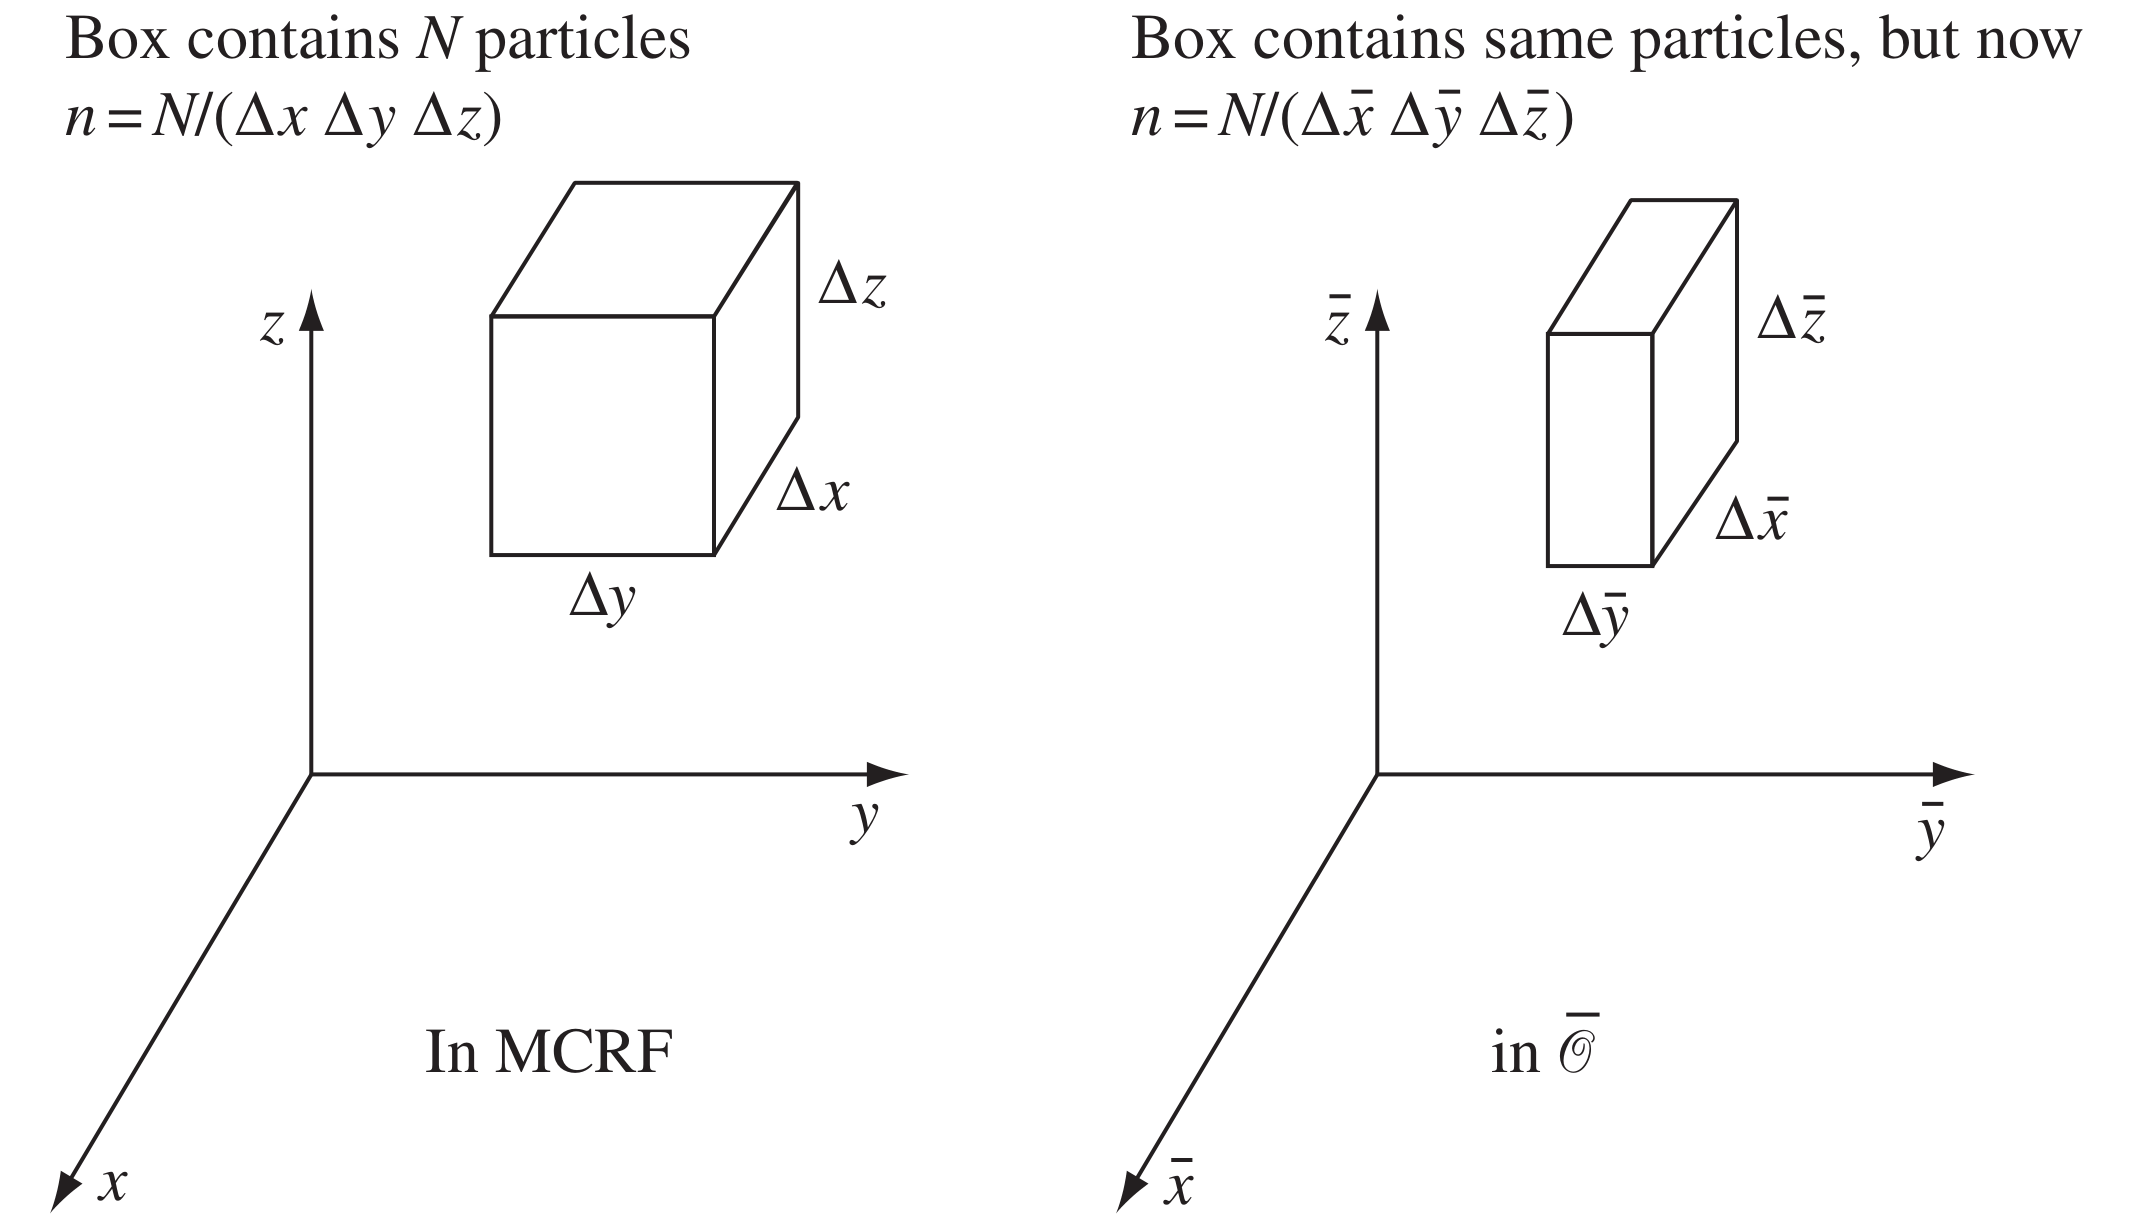
\includegraphics[width=0.7\textwidth]{fig4.1.png}
    \figcaption{\textit{Lorentz收缩使得粒子数密度依赖于坐标系。}}
    \label{fig4.1}
}

\subsection*{通过表面的流量}
对于运动的粒子,另一个有趣的问题是,沿某一方向“有多少”粒子运动?相应的精确概念是“流量(flux)”:\textit{粒子通过一个平面的流量是单位时间通过单位面积表面的粒子数}。显然,流量依赖于坐标系(“面积”与“时间”都依赖于坐标系)以及表面的方向(平行于粒子速度的表面,其流量为零,因为没有粒子通过它)。


{
    \centering
    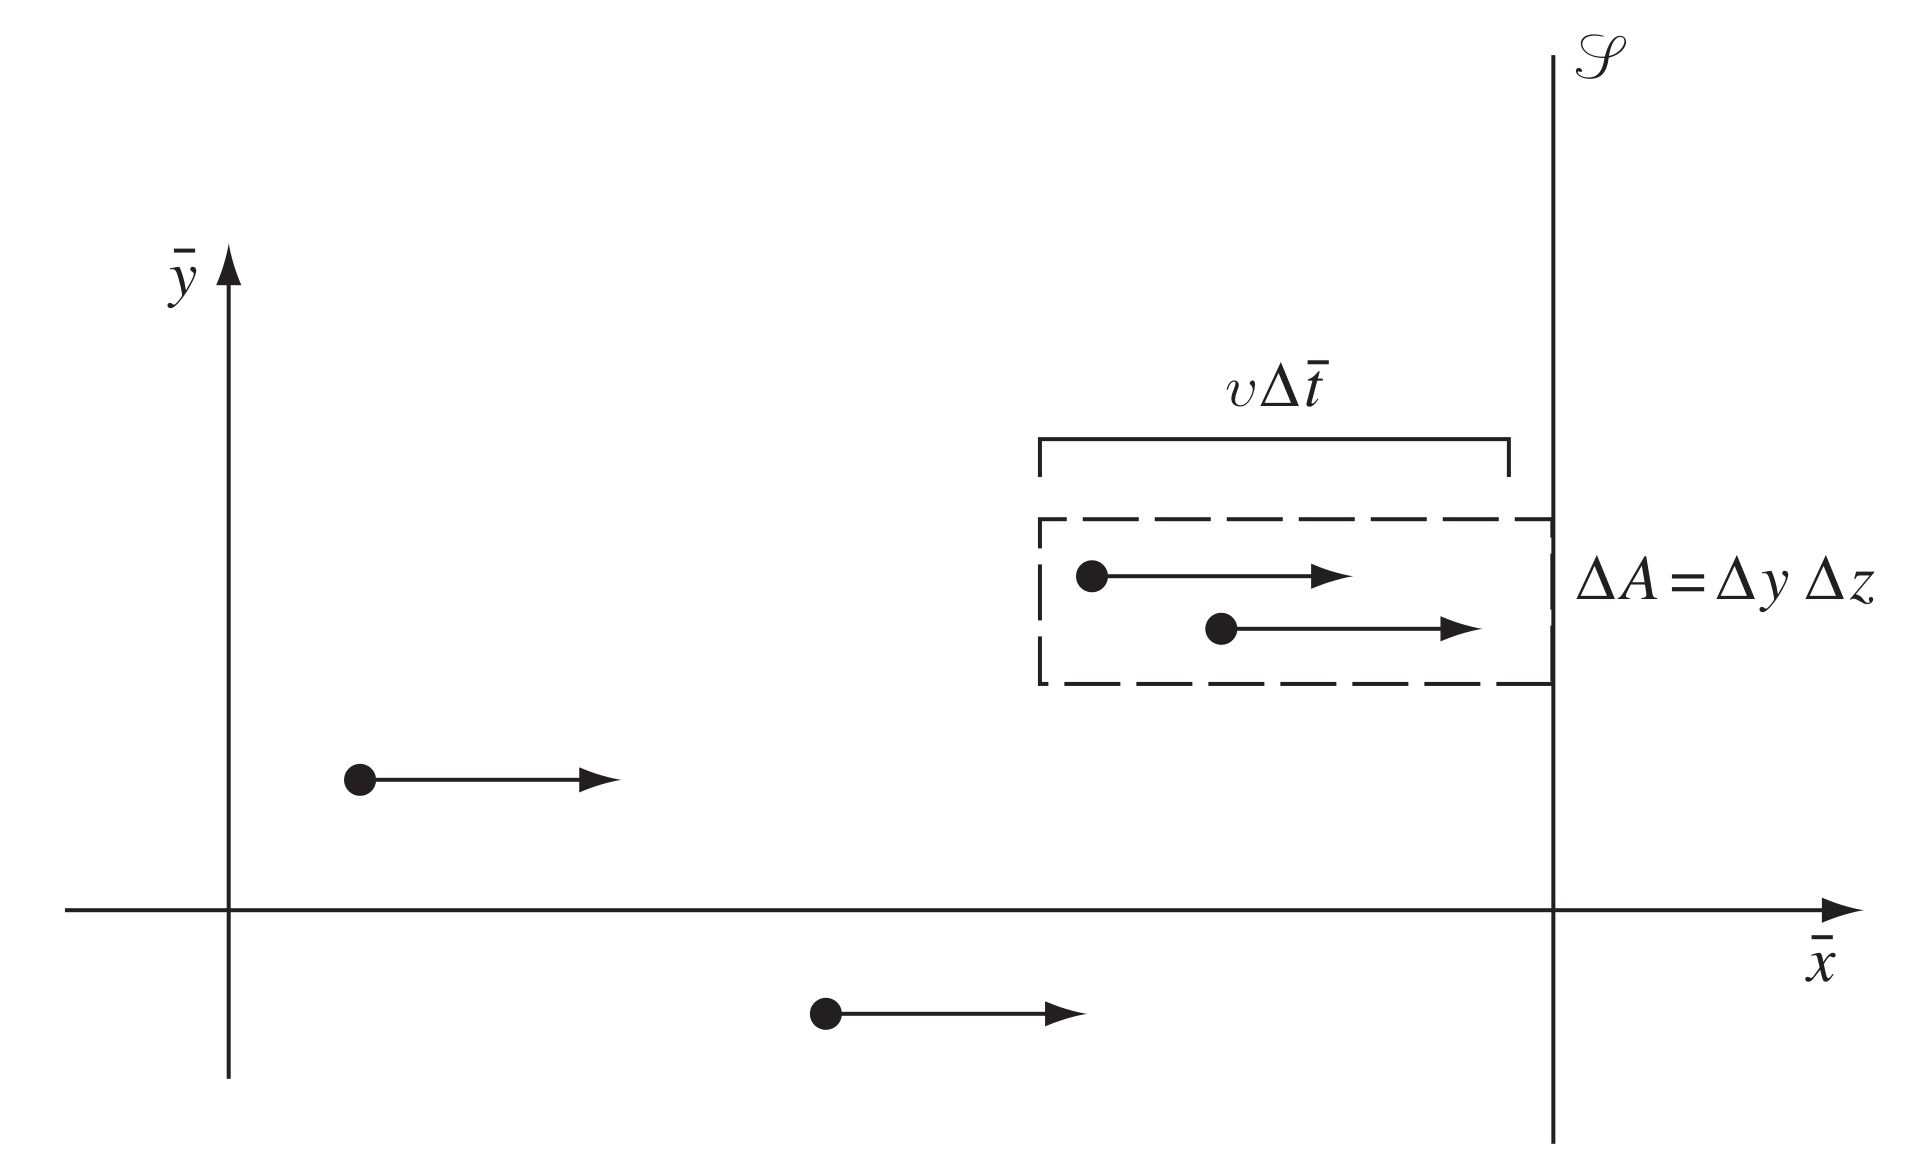
\includegraphics[width=0.7\textwidth]{fig4.2.png}
    \figcaption{\textit{流量变换律的简单图示:如果粒子只沿$x$轴运动,则在时间$\Delta \bar{t}$通过$\mathscr{S}$面的粒子位于距离$\mathscr{S}$面$v \Delta\bar{t}$的范围内。 }}
    \label{fig4.2}
}


在尘埃系统的静止坐标系中流量为零,因为所有粒子静止。设在$\MObar$系,所有粒子沿$\bar{x}$ 方向以速度$v$运动,先考虑垂直于$\bar{x}$轴的平面(如图\ref{fig4.2}),图中由虚线表示的立方体区域内的粒子就是在时间$\Delta \bar{t}$内通过$\mathscr{S}$面的面积$\Delta A$的粒子。这个区域的体积是$v \Delta \bar{t}\, \Delta A$,由于该系的数密度为$n / \sqrt{1 - v^2}$,因此该区域的粒子数为$[n / \sqrt{1 - v^2}] v \Delta \bar{t}$。\textbf{单位时间}内穿过等$\bar{x}$面($\mathscr{S}$面)单位面积的粒子数,也就是通过等$\bar{x}$面的流量为:

\[
    (\text{flux})^{\bar{x}} = \frac{nv}{\sqrt{1 - v^2}}.
\]

更一般的情况是,粒子在$\MObar$系中也有$\bar{y}$方向的速度,图\ref{fig4.3}中,在$\Delta \bar{t}$时间内通过$\mathscr{S}$面的面积$\Delta A$的粒子位于虚线区域内,该区域是“平行六面体”形状的,它的体积等于底乘以高,它的高——$\bar{x}$方向的长度——等于$v^{\bar{x}} \,\Delta \bar{t}$,由此可得

\begin{equation}
    (\text{flux})^{\bar{x}} = \frac{n v^{\bar{x}}}{\sqrt{1 - v^2}}.
\label{equ4.3}
\end{equation}

{
    \centering
    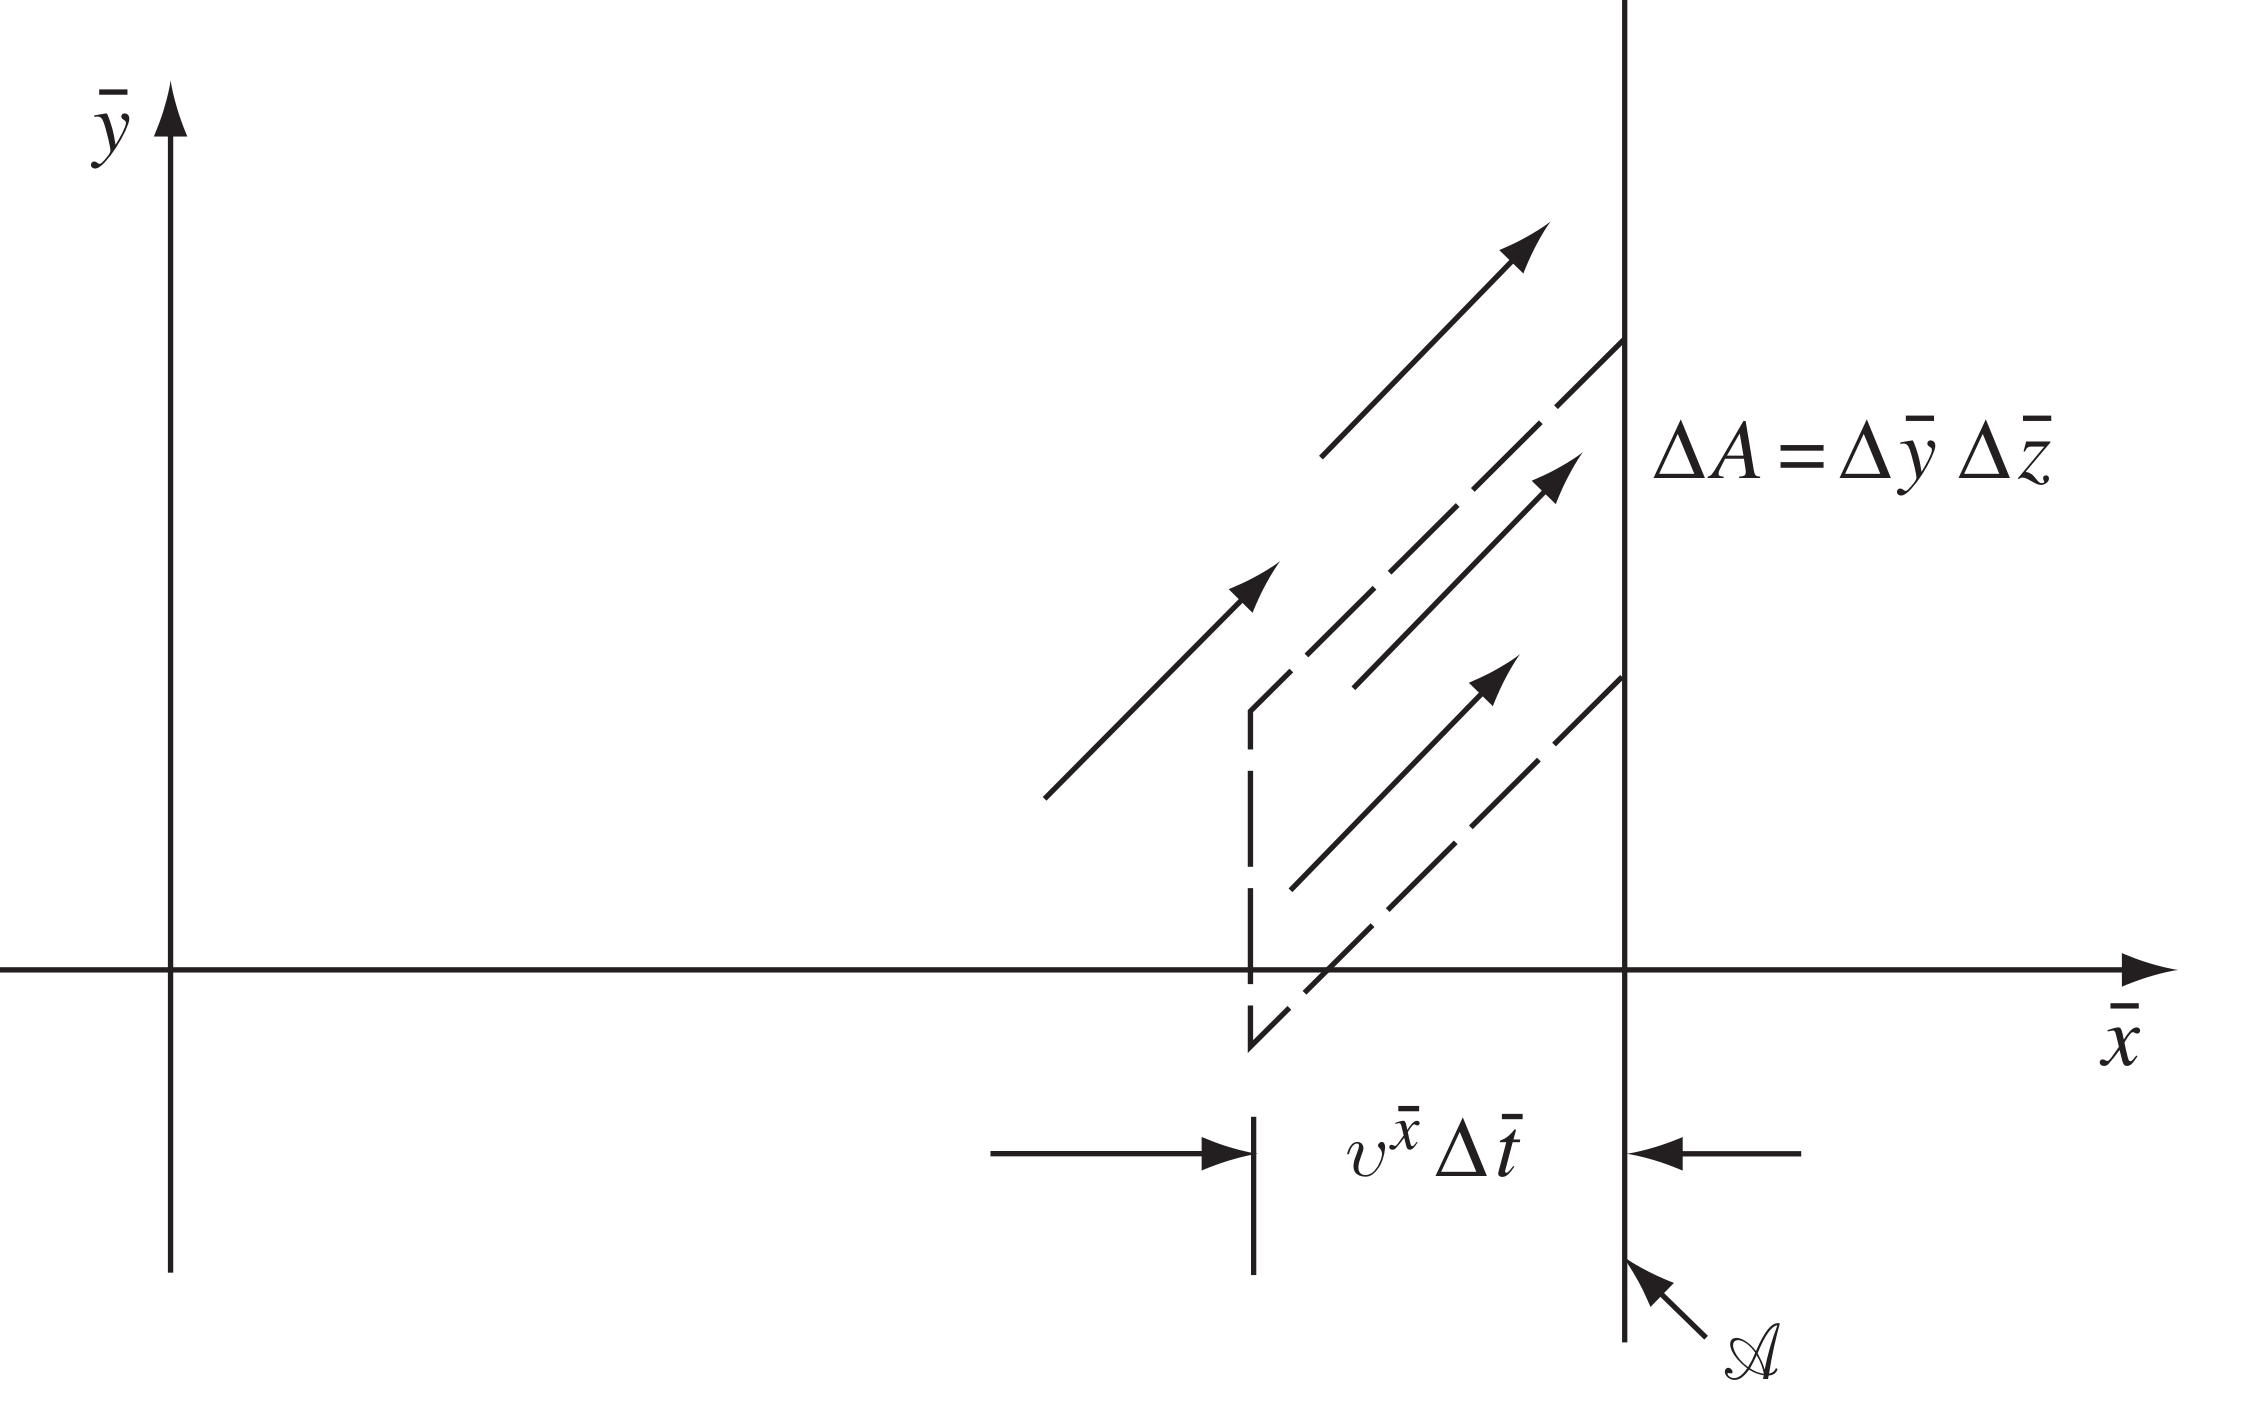
\includegraphics[width=0.7\textwidth]{fig4.3.png}
    \figcaption{\textit{流量的更一般情况:通过等$\bar{x}$坐标面的流量只与粒子速度的$\bar{x}$分量有关。}}
    \label{fig4.3}
}


\subsection*{数流密度四维向量$\vec{N}$}
定义向量$\vec{N}$为
\begin{shaded}
\begin{equation}
    \vec{N} = n \vec{U},
\label{equ4.4}
\end{equation}
\end{shaded}
其中$\vec{U}$是粒子四速。设在$\MObar$系中粒子速度为$(v^x, v^y, v^z)$,则有
\[
    \vec{U} \xrightarrow[\MObar]{ } \left( \frac{1}{\sqrt{1 - v^2}}, \frac{v^x}{\sqrt{1 - v^2}}, \frac{v^y}{\sqrt{1 - v^2}}, \frac{v^z}{\sqrt{1 - v^2}} \right).
\]
因此
\begin{equation}
    \vec{N} \xrightarrow[\MObar]{ } \left( \frac{n}{\sqrt{1 - v^2}}, \frac{nv^x}{\sqrt{1 - v^2}}, \frac{n v^y}{\sqrt{1 - v^2}}, \frac{n v^z}{\sqrt{1 - v^2}} \right).
\label{equ4.5}
\end{equation}
可见,在任意坐标系中,$\vec{N}$的时间分量是数密度,空间分量是通过不同坐标面的流量。这个概念超级重要。在伽利略的物理学中,数密度是个在所有坐标系都相同的标量(没有Lorentz收缩),而流量是很不一样的物理量:它是\textbf{依赖于}坐标系的三维向量,因为粒子速度依赖于坐标系。在相对论中,数密度与流量被统一到同一个不依赖于坐标系的四维向量当中。这是思维方式最主要的一大进步:将看起来无关的概念统一到一个量。

值得再次强调“不依赖于坐标系”的含义。向量$\vec{N}$是个几何量,它的存在不依赖于任何坐标系;就像一般的张量那样,$\vec{N}$将1形式映射为数字,与坐标系无关。它的分量\textbf{确实}依赖于坐标系。由于相对论之前的物理学认为流量是三维向量,并且还依赖于坐标系:流量是三维向量,因为它与坐标轴的指向无关(就像四维向量与坐标系无关那样);但是流量这种三维向量在相互运动的坐标系中的分量不同,因为粒子的速度在这些坐标系中不同。对于旧物理学,流量向量必须在某个惯性系定义。而相对论只需要定义\textbf{一个}向量,旧物理学中坐标依赖的定义方式是因为只考虑了$\vec{N}$的四个分量中的三个。伽利略物理学中的坐标系无关量——数密度,和依赖于坐标系的量——流量,在相对论中被统一到了一个不依赖坐标系的四维向量$\vec{N}$当中,就像“能量”和“动量”被统一到了四维动量中那样。

最后,根据定义显然有
\begin{shaded}
\begin{equation}
    \vec{N} \cdot \vec{N} = -n^2, \quad n = (- \vec{N} \cdot \vec{N})^{1/2}.
\label{equ4.6}
\end{equation}
\end{shaded}
可见$n$是个标量。就像“静质量”是标量,而能量与“惯性质量”依赖于坐标系那样,“静密度”(静止坐标系观测到的粒子数密度)$n$是标量,而“数密度”依赖于坐标系。$n$\textbf{总是}定义为粒子的MCRF观测到的数密度,也就是一个标量。流体的压强、温度等其它特征量的定义也是如此,之后会讨论它们。

\section{1形式与表面}
\label{sec4.3}

\subsection*{数密度是一种类时流量}
为了进一步完善上面数密度与流量的统一,我们来论证数密度可以视为一种类时流量(timelike flux)。还是先考虑通过等$\bar{x}$坐标面的流量,在\textbf{时空图}中画出相应过程,如图\ref{fig4.4},图中只画出了$\bar{t}$轴和$\bar{x}$轴。

{
    \centering
    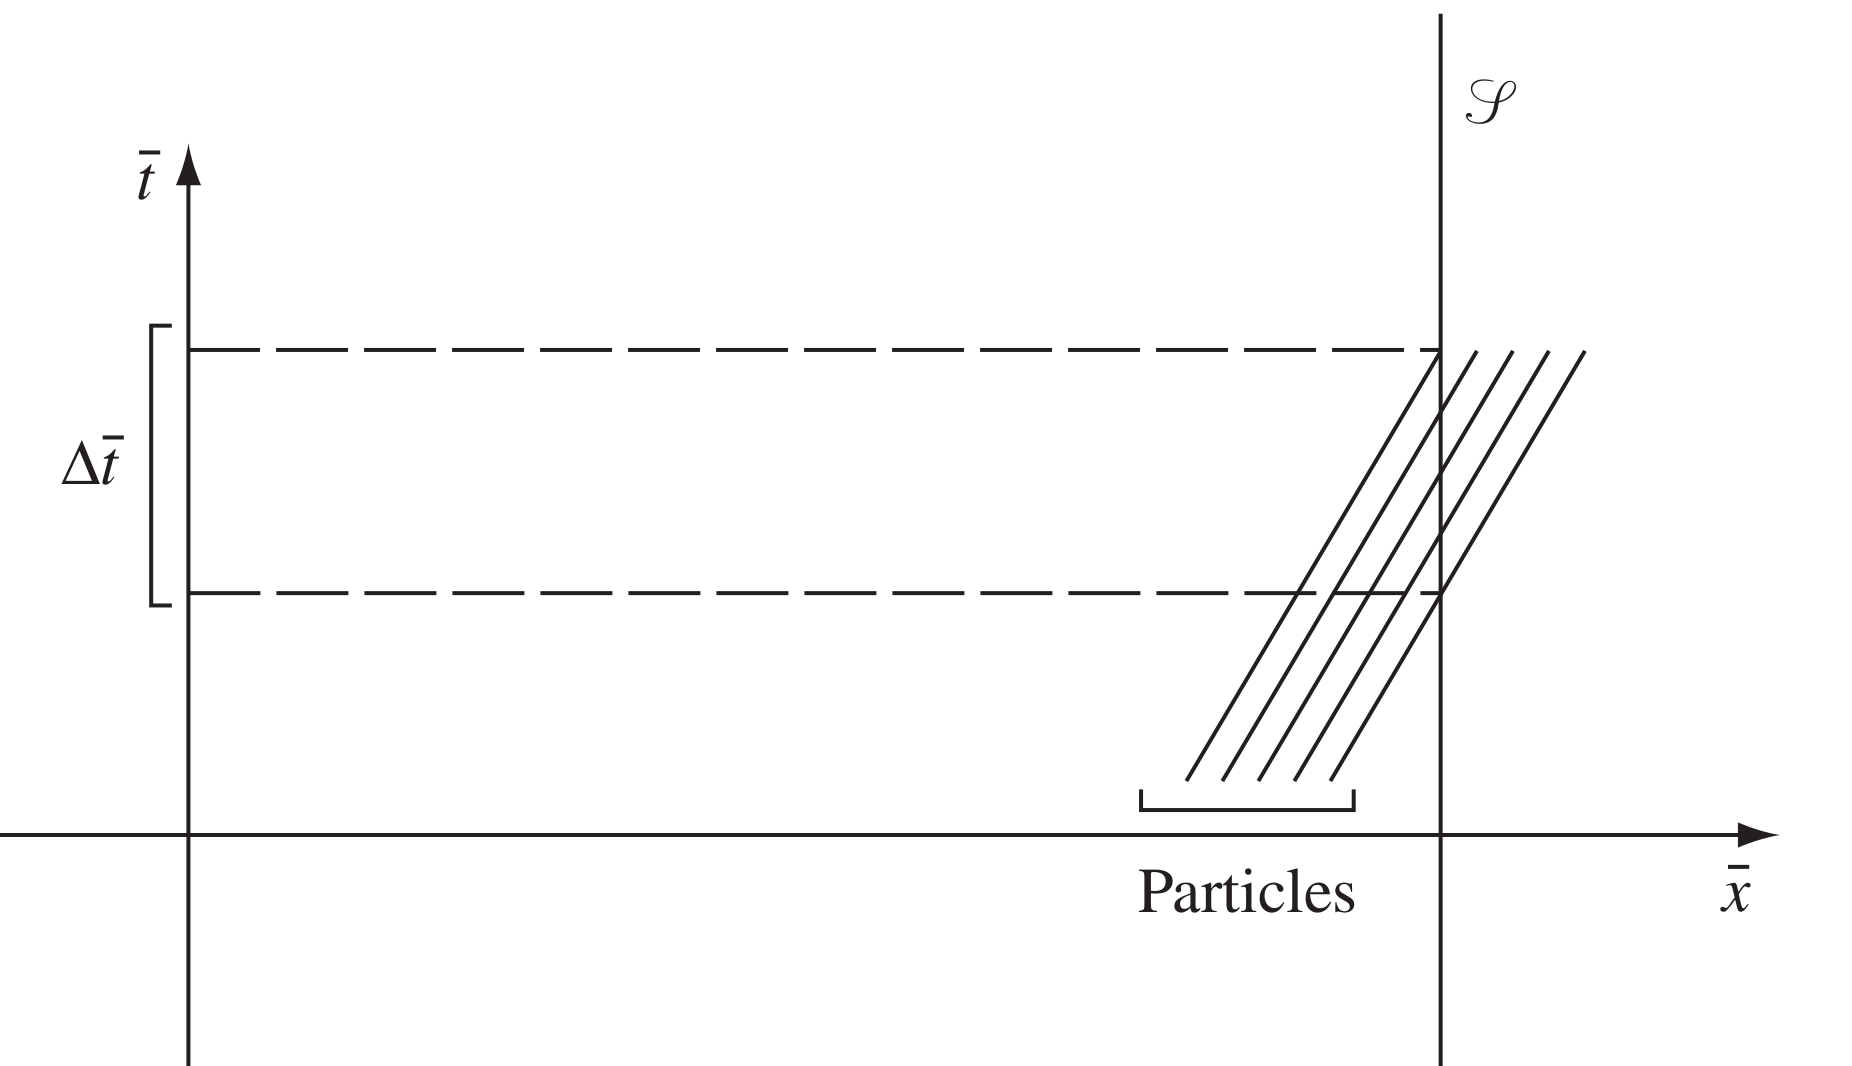
\includegraphics[width=0.7\textwidth]{fig4.4.png}
    \figcaption{\textit{图\ref{fig4.2}的时空图版本,其中省略了$\bar{y}$轴。}}
    \label{fig4.4}
}

垂直于$\bar{x}$轴的$\mathscr{S}$面的世界线如图所示,由于省略了$\bar{y}, \bar{z}$轴,因此任意时刻$\bar{t}$只对应一个点。在时间$\Delta \bar{t}$内通过$\mathscr{S}$面的粒子的世界线是图中的倾斜直线,流量即为在时间间隔$\Delta \bar{t} = 1$之内穿过$\mathscr{S}$面的粒子世界线数目。实际上,由于$\mathscr{S}$面是二维的,因此它的“世界轨迹”是三维的(“世界体”),而图中只能画出一部分。\textbf{流量}是通过单位“体积”世界体的世界线数目:单位体积的含义是边长为1单位的立方体$\Delta \bar{t} = 1, \Delta \bar{y} = 1, \Delta \bar{z} = 1$。因此,流量可以定义为通过三维世界体单位体积的粒子世界线数目。同理,这种三维世界体也可以是某一时刻$\bar{t}$对应的三维空间体的单位体积$\Delta \bar{x} = 1, \Delta \bar{y} = 1, \Delta \bar{z} = 1$,如图\ref{fig4.5}。这样,流量就是通过$\Delta \bar{x} = 1$($\Delta \bar{y}, \Delta \bar{z}$省略了)的世界线数目,而它正是特定时刻的单位体积内的粒子数:数密度。因此“类时”流量是数密度。

{
    \centering
    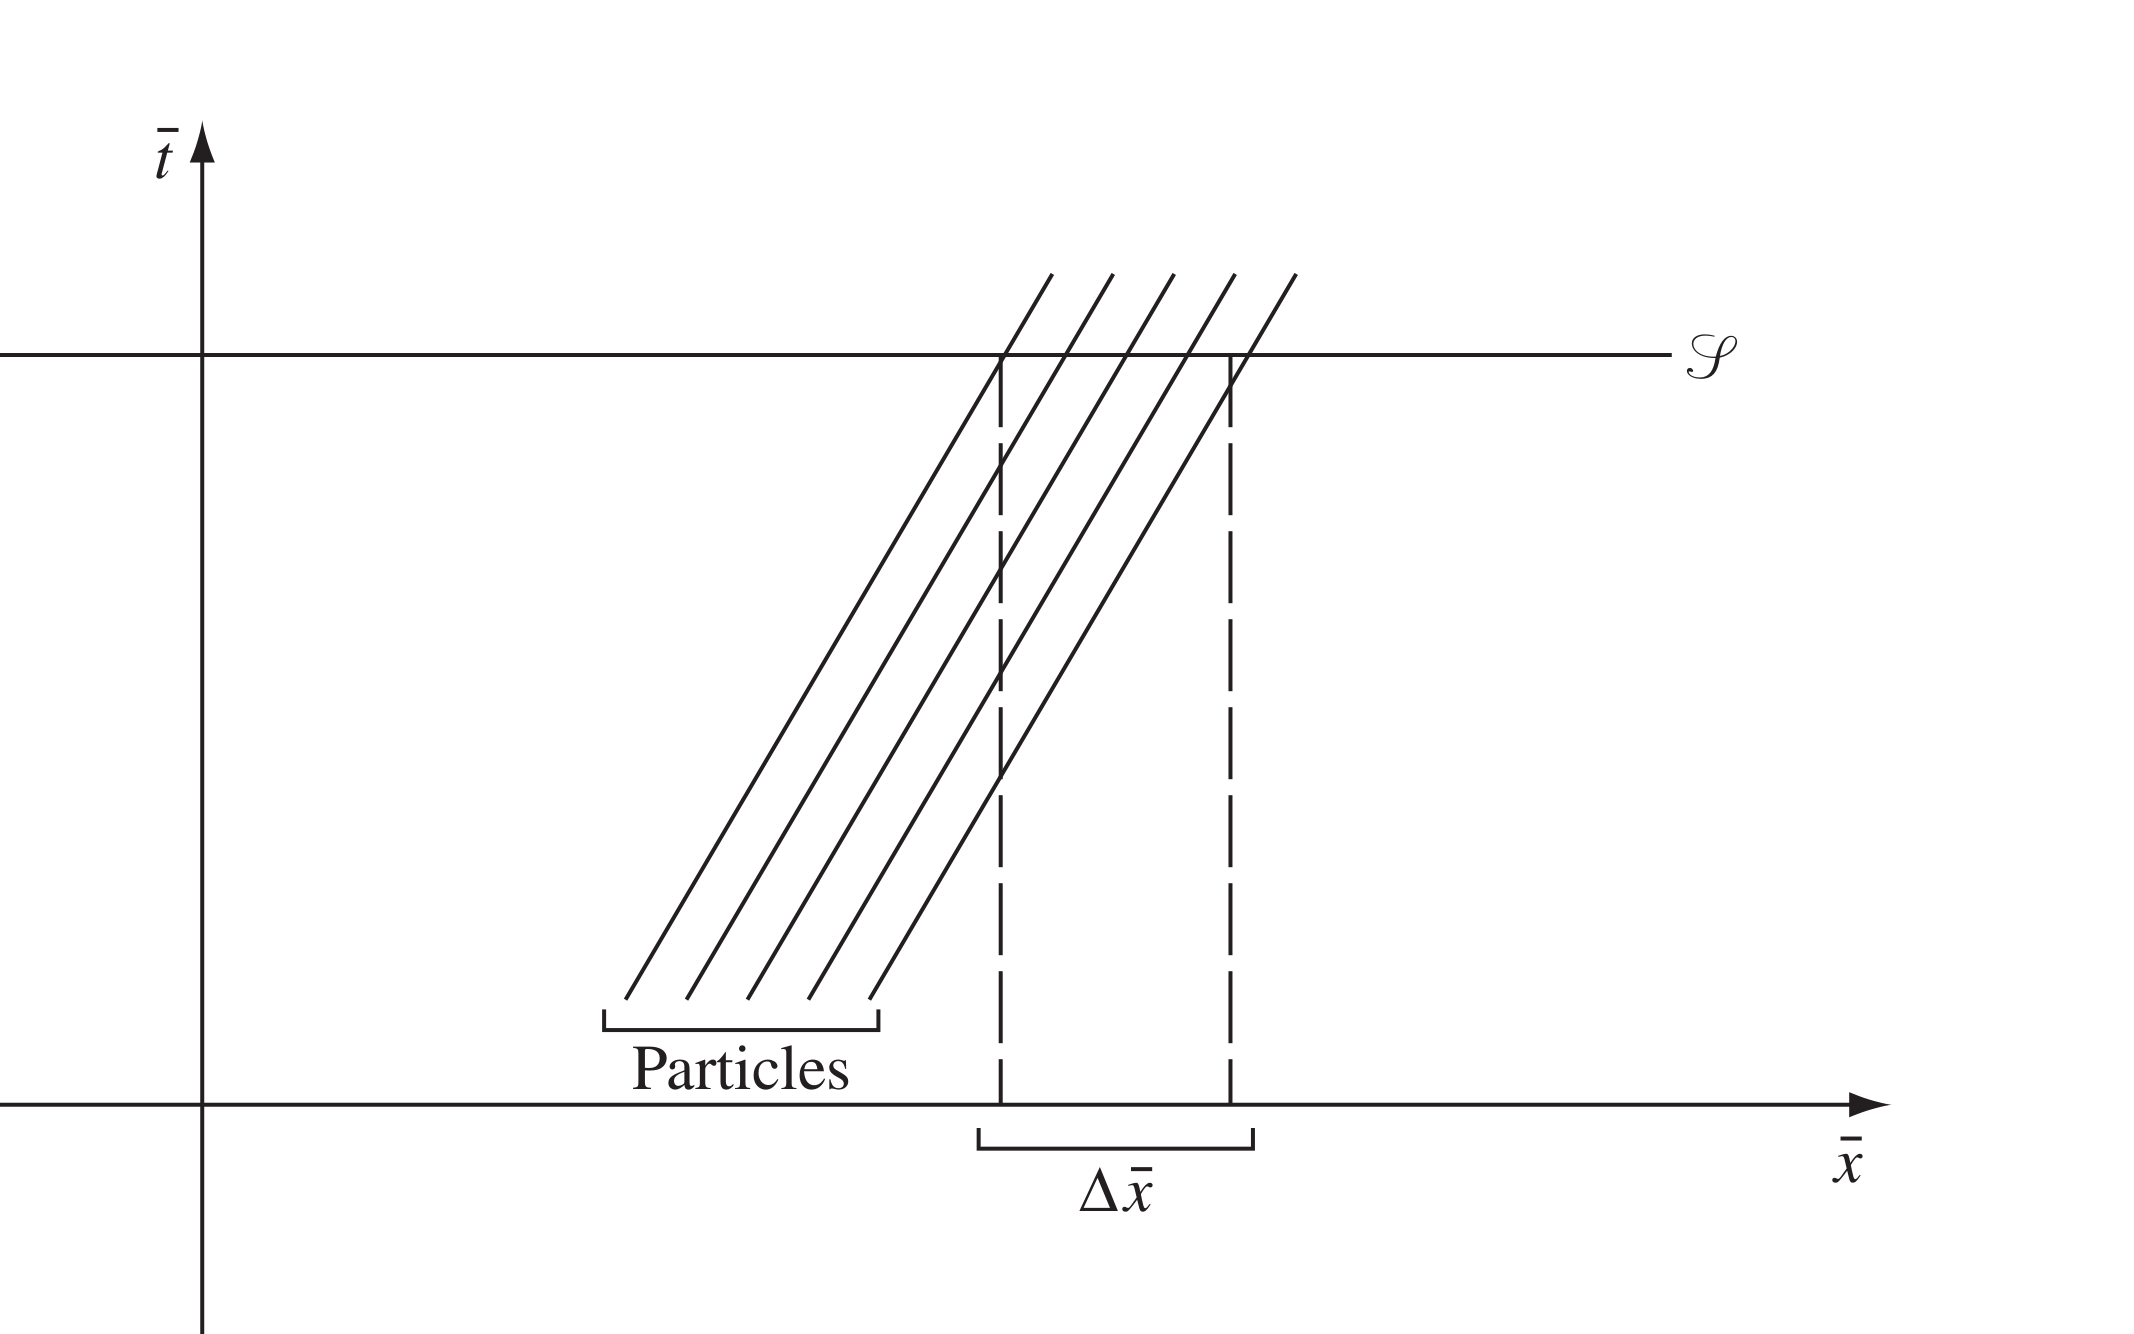
\includegraphics[width=0.7\textwidth]{fig4.5.png}
    \figcaption{\textit{数密度可以视为通过等时面$\bar{t} = \text{常数}$\ 的流量。}}
    \label{fig4.5}
}

\subsection*{一个1形式定义了一个表面}
前文描述表面的方式有点笨拙。为了用更加具有不变性的方式描述,需要用一种数学概念来表示粒子世界线所通过的表面,这要用到1形式。一般地,一个表面是由某个方程的解定义的:
\[
    \phi(t, x, y, z) = \text{常数。}
\]
函数$\phi$的梯度$\trd \phi$是法向1形式。某种程度上,$\trd \phi$\textbf{定义了}表面$\phi = \text{常数}$,因为它唯一确定了表面的法方向。然而,$\trd \phi$的任意常数倍也定义了同样的表面,因此一般采用单位法向1形式(unit-normal one-form)来描述not null的表面:
\begin{equation}
    \tilde{n} := \frac{\trd \phi}{|\trd \phi|},
\label{equ4.7}
\end{equation}
其中
\begin{align}
    |\trd \phi| \text{是}\trd\phi \text{的模:}\quad |\trd \phi| = |\eta^{\alpha \beta} \phi_{, \alpha} \phi_{, \beta} |^{1/2}. \label{equ4.8}
\end{align}
(不要把$\tilde{n}$和$n$混淆,后者是MCRF观测到的数密度,两者截然不同,只是由于偶然的历史原因使得它们的字母相同。)

就像三维空间的向量分析(例如高斯定律)那样,定义“面元(surface element)”为单位法向1形式乘以表面面元的面积。这样,坐标为$x^\alpha, x^\beta, x^\gamma$($\alpha, \beta, \gamma$是\textbf{特定的}、互不相同的指标)的三维体积元可以表示为
\begin{equation}
    \tilde{n} \rd x^\alpha \, \rd x^\beta \, \rd x^\gamma,
\label{equ4.9}
\end{equation}
而\textbf{单位}体积元($\rd x^\alpha = \rd x^\beta = \rd x^\gamma = 1$)就是$\tilde{n}$。(这些$\rd x$是要被积分掉的无穷小量,而非梯度。)

\subsection*{通过表面的流量}
回顾一下三维空间的高斯定律,它表明通过表面的流量,例如电场通量为$\bm{E} \cdot \bm{n}$,即电场$\bm{E}$与单位法向量的点乘。这里的情况也差不多:(粒子)通过等$\phi$面的流量是$\langle \tilde{n}, \vec{N} \rangle$。为了证明该式,先考虑$\phi$是坐标之一,例如$\bar{x}$的情况。等$\bar{x}$面的法向1形式为$\trd \bar{x}$,它也是单位1形式,因为$\trd \bar{x} \xrightarrow[\MObar]{ } (0, 1, 0, 0)$。则$\langle \trd \bar{x}, \vec{N} \rangle = N^\alpha (\trd \bar{x})_\alpha = N^{\bar{x}}$,由上文可见这就是通过$\bar{x}$坐标面的流量。显然,如果选择$\phi = \bar{t}$,则$\langle \trd \bar{x}, \vec{N} \rangle$的结果为$N^{\bar{0}}$——数密度,亦即通过等$\bar{t}$面的流量。

向量的定义是把1形式映射为实数的函数,上面是该定义的第一个物理实例。给定向量$\vec{N}$,可以计算通过某个面的流量——将向量与该平面的单位法向1形式缩并即可。此外,这个不依赖于坐标系的表达式$\langle \trd \bar{x}, \vec{N} \rangle$还把粒子系统的性质$\vec{N}$与表面的性质$\tilde{n}$分离开来。在下面的\ref{sec4.4}节还会讨论类似内容。

\subsection*{用1形式表示坐标系}
在继续讨论流体的其它性质之前,我们应该介绍一个有用的结论。目前我们用四维速度来定义一个惯性系,它也可以用1形式定义,也就是用四维速度对应的1形式$\mathbf{g} (\vec{U}, \ )$,它的分量为
\[
    U_\alpha = \eta_{\alpha \beta} U^\beta,
\]
在它所表示的坐标系中:
\[
    U_0 = -1, \quad U_i = 0.
\]
显然这个1形式等于$-\trd \bar{t}$(它们的分量相等)。由此可见,给定一个$\trd t$就等效地定义了一个惯性坐标系。相应的物理图像是:$\trd t$可以视为一组等$t$面,在同一个表面上的时刻相等。这显然定义了一个坐标系,只是还有一些空间坐标旋转的自由度(通常可以忽略)。实际上,$\trd t$某种程度上比$\vec{U}$的定义更加自然。例如,四动量为$\vec{p}$的粒子在$\trd t$表示的坐标系中的能量为
\begin{equation}
    E = \langle \trd t, \vec{p} \rangle = p^0.
\label{equ4.10}
\end{equation}
这样不会出现方程\eqref{equ2.35}当中不方便的负号:
\[
    E = -\vec{p} \cdot \vec{U}.
\]

\section{还是尘埃系统:应力-能量张量}
\label{sec4.4}
目前我们讨论了如何描述尘埃系统的粒子数,粒子也有能量、动量,后面会看到,它们的能量动量是GR中的引力场源。因此需要研究如何用具有坐标系不变性的方式描述这些量。简明起见,假设所有尘埃粒子具有相同的静质量$m$。

\subsection*{能量密度}
在MCRF中,每个粒子的能量为$m$,单位体积的粒子数为$n$,因此单位体积的能量为$mn$,将它记作$\rho$:
\begin{equation}
    \rho := \text{MCRF观测到的能量密度。}
\label{equ4.11}
\end{equation}
$\rho$是标量,就像$n, m$那样。对于尘埃系统:
\begin{equation}
    \rho = nm \text{(尘埃系统)。}
\label{equ4.12}
\end{equation}
对于更一般的流体,需要考虑粒子的随机热运动动能,即使在所有粒子的平均速度为零的坐标系内,\eqref{equ4.12}式也不再有效。

$\MObar$系观测到的数密度为$n / \sqrt{1 - v^2}$,由于所有粒子在$\MObar$系速度为$v$,因此粒子在该系的能量为$m / \sqrt{1 - v^2}$。因此能量密度为$mn / \sqrt{1 - v^2}$:
\begin{equation}
    \frac{\rho}{1 - v^2} = \Big\{ \text{粒子在其中的速度为$\bm{v}$的坐标系观测到的能量密度。} \Big\}.
\label{equ4.13}
\end{equation}
这个变换式含有两个因子$(1 - v^2)^{-1/2} = \Lambda\indices{^{\bar{0}}_0}$,因为体积与能量\textbf{二者都}进行了变换。因此能量密度不可能是某个向量的分量,实际上它是某个$\binom{2}{0}$张量的分量。这可以通过张量的定义看出。定义能量需要一个1形式,从而得到四动量的0分量;定义密度也需要一个1形式,因为密度是通过某个等时面的流量。于是,定义能量流量(简称为“能流”)需要两个1形式:1个定义能量、1个定义表面。同理,定义动量密度(momentum density)需要两个1形式:1个定义动量分量、1个定义密度。动量流(momentum flux)(定义为动量(的某个分量)通过某个表面的速率)也一样需要两个1形式。这些量可以统一为一个$\binom{2}{0}$张量$\textbf{T}$,其名为\textbf{应力-能量张量}(stress-energy tensor),这个张量将两个合适的1形式映射为相应的值。

\subsection*{应力-能量张量}
应力-能量张量最方便的定义是在某个(任意)坐标系中给出它的分量:

\begin{shaded}
\begin{equation}
    \mathbf{T} (\trd x^\alpha, \trd x^\beta) = T^{\alpha \beta} := \Bigg\{ \text{$\alpha$动量通过等$x^\beta$面的流量} \Bigg\}.
\label{equ4.14}
\end{equation}
\end{shaded}
(其中$\alpha$动量是指四动量的$\alpha$分量:$p^\alpha := \langle \trd x^\alpha, \vec{p} \rangle$。)上式符合张量的定义,证明作为本章习题5。

下面来讨论这个定义是怎样符合上文内容的。

\begin{itemize}
    \item $T^{00}$定义为0动量(能量)通过等时面$t = \text{constant}$\ 的流量,也就是能量密度:
    \begin{equation}
        T^{00} = \text{能量密度。}
    \label{equ4.15}
    \end{equation}
    \item $T^{0i}$是能量通过坐标面$x^i$(即表面$x^i = \text{常数}$)的流量:
    \begin{equation}
        T^{0i} = \text{通过$x^i$坐标面的能量流。}
    \label{equ4.16}
    \end{equation}
    \item $T^{i0}$是$i$动量通过$t = \text{constant}$\ 面的流量,也就是$i$动量密度:
    \begin{equation}
        T^{i0} = \text{$i$动量密度。}
    \label{equ4.17}
    \end{equation}
    \item $T^{ij}$是$i$动量的$j$流量:
    \begin{equation}
        T^{ij} = \text{通过$x^j$坐标面的$i$动量流量。}
    \label{equ4.18}
    \end{equation}
\end{itemize}
只要给定了$\mathbf{T}$在任意坐标系的分量,则它在其余坐标系的分量随之确定。对于尘埃系统,$\mathbf{T}$在MCRF的分量非常简单,在MCRF中的尘埃粒子速度为零,因此所有的$i$动量为零、空间流量为零,于是:
\begin{align*}
    (T^{00})_{\text{MCRF}} &= \rho = mn, \\
    (T^{0i})_{\text{MCRF}} &= (T^{i0})_{\text{MCRF}} = (T^{ij})_{\text{MCRF}} = 0.
\end{align*}
容易验证,张量$\vec{p} \otimes \vec{N}$在MCRF中的分量也是如此,其中$\vec{p} = m\vec{U}$是单个粒子的四速。于是
\begin{shaded}
\begin{equation}
    \text{尘埃系统:}\quad \mathbf{T} = \vec{p} \otimes \vec{N} = mn \vec{U} \otimes \vec{U} = \rho \vec{U} \otimes \vec{U}.
\label{equ4.19}
\end{equation}
\end{shaded}
由此可得
\begin{align}
    T^{\alpha \beta} &= \mathbf{T} (\tilde{\omega}^\alpha, \tilde{\omega}^\beta) \notag \\
    &= \rho \vec{U} (\tilde{\omega}^\alpha) \vec{U} (\tilde{\omega}^\beta) \notag \\
    &= \rho U^\alpha U^\beta. \label{equ4.20}
\end{align}

在$\MObar$系中:
\[
    \vec{U} \to \left( \frac{1}{\sqrt{1 - v^2}}, \frac{v^x}{\sqrt{1 - v^2}}, \dots \right),
\]
由此可得
\begin{equation}
\left.
\begin{split}
    T^{\bar{0} \bar{0}} &= \rho U^{\bar{0}} U^{\bar{0}} &= \frac{\rho}{1 - v^2}, \\
    T^{\bar{0} \bar{i}} &= \rho U^{\bar{0}} U^{\bar{i}} &= \frac{ \rho v^i }{ 1 - v^2 }, \\
    T^{\bar{i} \bar{0}} &= \rho U^{\bar{i}} U^{\bar{0}} &= \frac{\rho v^i}{1 - v^2}, \\
    T^{\bar{i} \bar{j}} &= \rho U^{\bar{i}} U^{\bar{j}} &= \frac{\rho v^i v^j}{1 - v^2}.
\end{split}
\right\}
\label{equ4.21}
\end{equation}
这与根据能量密度、能量流、动量密度、动量流的第一性原理的计算结果一致。(前文根据第一性原理计算了能量密度。)注意一个重要结果:$T^{\alpha \beta} = T^{\beta \alpha}$,也就是说,$\mathbf{T}$是对称张量。后面会发现这个结论不止对尘埃系统,对所有系统都成立。


\section{一般流体}
\label{sec4.5}
目前我们处理的是最简单的粒子集合——尘埃系统,为了将结论推广到一般流体,需要考虑如下几个性质:
\begin{enumerate}
    \item 除了流体的整体运动以外,每个粒子都有自己的随机热运动速度;
    \item 粒子之间有相互作用力,也就是流体的总能量还包括相互作用势能。
\end{enumerate}

\subsection*{宏观量的定义}
\ref{sec4.1}节讨论了流体元的概念。对于每个流体元,存在着它在其中静止(即四动量的空间分量为零)的坐标系,即该流体元的MCRF。这个系是真正\textbf{瞬时}共动的:因为一般情况下的流体元可能加速减速,下一时刻的MCRF就会是另一个坐标系,因此同一流体元在不同时刻的MCRF一般不同。MCRF相应于一个流体元,而哪个坐标系是MCRF则是关于位置与时间的函数。\textbf{在相对论中所有与流体元有关的标量}(例如数密度、能量密度、温度)\textbf{定义为它们在流体元的MCRF中的取值。} 表格4.1列出了各种宏观量的定义。我们只考虑单一组分(一种粒子)的流体,因此渗流等等类似的物理量没有出现。


\begin{table}[h]
\centering
\begin{tabular}{c c c}
\toprule
符号 & 名称 & 定义 \\
\midrule
$\vec{U}$ & 流体元的四速 & MCRF的四速 \\
$n$ & 数密度 & MCRF中单位体积的粒子数 \\
$\vec{N}$ & 流量向量 & $\vec{N} := n \vec{U}$ \\
$\rho$ & 能量密度 & \textbf{总}质能(静质能、随机热运动动能、化学能、…)密度 \\
$\Pi$ & 单位粒子的相互作用能 & $\Pi := (\rho/n) - m \Rightarrow \rho = n(m + \Pi) $,因此$\Pi$是静质能之外能量的统称。 \\
$\rho_0$ & 静质量密度 & $\rho_0 := mn$。由于$m$是常数,因此这是只与静质量有关的“能量”,$\rho = \rho_0 + n \Pi$. \\
$T$ & 温度 & MCRF中通常的热力学定义(见下文) \\
$p$ & 压强 & MCRF中通常的流体动力学定义(见下文) \\
$S$ & 比熵 & 单位粒子的熵(见下文)\\
\bottomrule
\end{tabular}
\caption{单组分流体的宏观量}
\end{table}

\subsection*{热力学第一定律}
热一定律就是能量守恒的陈述。在MCRF中,假设流体元只通过两种方式与周围环境交换能量:热传导(吸收的热量记作$\Delta Q$)、做功(对外做功$p \, \Delta V$,其中$V$是流体元的三维体积)。流体元的总能量记作$E$,由于$\Delta Q$是吸收的热量、$p\,\Delta V$是对外做的功,根据能量守恒:(各项都是小量)
\begin{equation}
\left.
\begin{split}
    \Delta E &= \Delta Q - p \,\Delta V, \\
\text{移项得:}\quad    \Delta Q &= \Delta E + p\,\Delta V.
\end{split}
\right\}
\label{equ4.22}
\end{equation}
如果流体元含有$N$个粒子,且粒子数不变(即粒子不会产生或消失),则有
\begin{equation}
    V = \frac{N}{n}, \quad \Delta V = -\frac{N}{n^2} \,\Delta n.
\label{equ4.23}
\end{equation}
此外,根据$\rho$的定义可得
\begin{align*}
    E &= \rho V = \rho N / n, \\
    \Delta E &= \rho \Delta V + V \Delta \rho.
\end{align*}
由以上两个结果可得
\[
    \Delta Q = \frac{N}{n} \Delta \rho - N (\rho + p) \frac{\Delta n}{n^2}.
\]
定义单位粒子吸收的热量$q := Q/N$,则
\begin{equation}
    n \,\Delta q = \Delta \rho - \frac{\rho + p}{n} \,\Delta n.
\label{equ4.24}
\end{equation}
假设上式中的变化是“无穷小的”,可以证明,一般情况下的流体状态由两个参数确定,例如$\rho, T$,或者$\rho, n$。这意味着\eqref{equ4.24}式等号右侧
\[
    \rd \rho - (\rho + p) \frac{\rd n}{n}
\]
只依赖于$\rho$和$n$。一阶微分方程的理论表明上式\textbf{总是}存在\textbf{积分因子}:也就是说,总存在两个只与$\rho, n$有关的函数$A, B$,使得
\[
    \rd \rho - (\rho + p)\, \frac{\rd n}{n} \equiv A \, \rd B
\]
对任意$\rho, n$恒成立。热力学一般把$A/n$\textbf{定义为}温度、把$B$定义为比熵:
\begin{shaded}
\begin{equation}
    \rd \rho - (\rho + p) \,\frac{\rd n}{n} = nT\, \rd S,
\label{equ4.25}
\end{equation}
\end{shaded}
换句话说,
\begin{equation}
    \Delta q = T\,\Delta S.
\label{equ4.26}
\end{equation}
即,流体元的吸热量正比于它的熵的增量。

上面的$T, S$是作为方便的数学定义引入的,可以论证$T$就是通常所说的温度、$S$就是热力学第二定律中的熵,不过这里就不讨论热二定律了。熵是作为热一定律(能量守恒)的积分因子出现的。之后要用到\eqref{equ4.25}和\eqref{equ4.26}式。


\subsection*{一般的应力-能量张量}
$T^{\alpha \beta}$的定义式——方程\eqref{equ4.14}——是非常一般性的。在MCRF中,流体元没有整体流动,粒子的空间动量为零。于是在MCRF中:
\begin{enumerate}
    \item $T^{00} = \text{能量密度} = \rho$. 
    \item $T^{0i} = \text{能量流。}$ 尽管MCRF中粒子静止,但能量可以通过热传导进行传递。因此$T^{0i}$是MCRF中的热传导项。
    \item $T^{i0} = \text{动量密度}$。同样,尽管粒子在MCRF中静止,但能量可以通过热传导进行传递,传递的能量会有相应的动量。下面会证明$T^{i0} \equiv T^{0i}$。
    \item $T^{ij} = \text{动量流量}$。这是有趣而有用的量,下一节会详细讨论它,它的名字叫\textbf{应力(stress)}。
\end{enumerate}

\subsection*{$\mathbf{T}$的空间分量$T^{ij}$}
根据定义,$T^{ij}$是通过$x^j$坐标面的$i$动量流量。考虑两个相邻的流体元(如图\ref{fig4.6}),将它们画为立方体形状,交界面记作$\mathscr{S}$面。

{
    \centering
    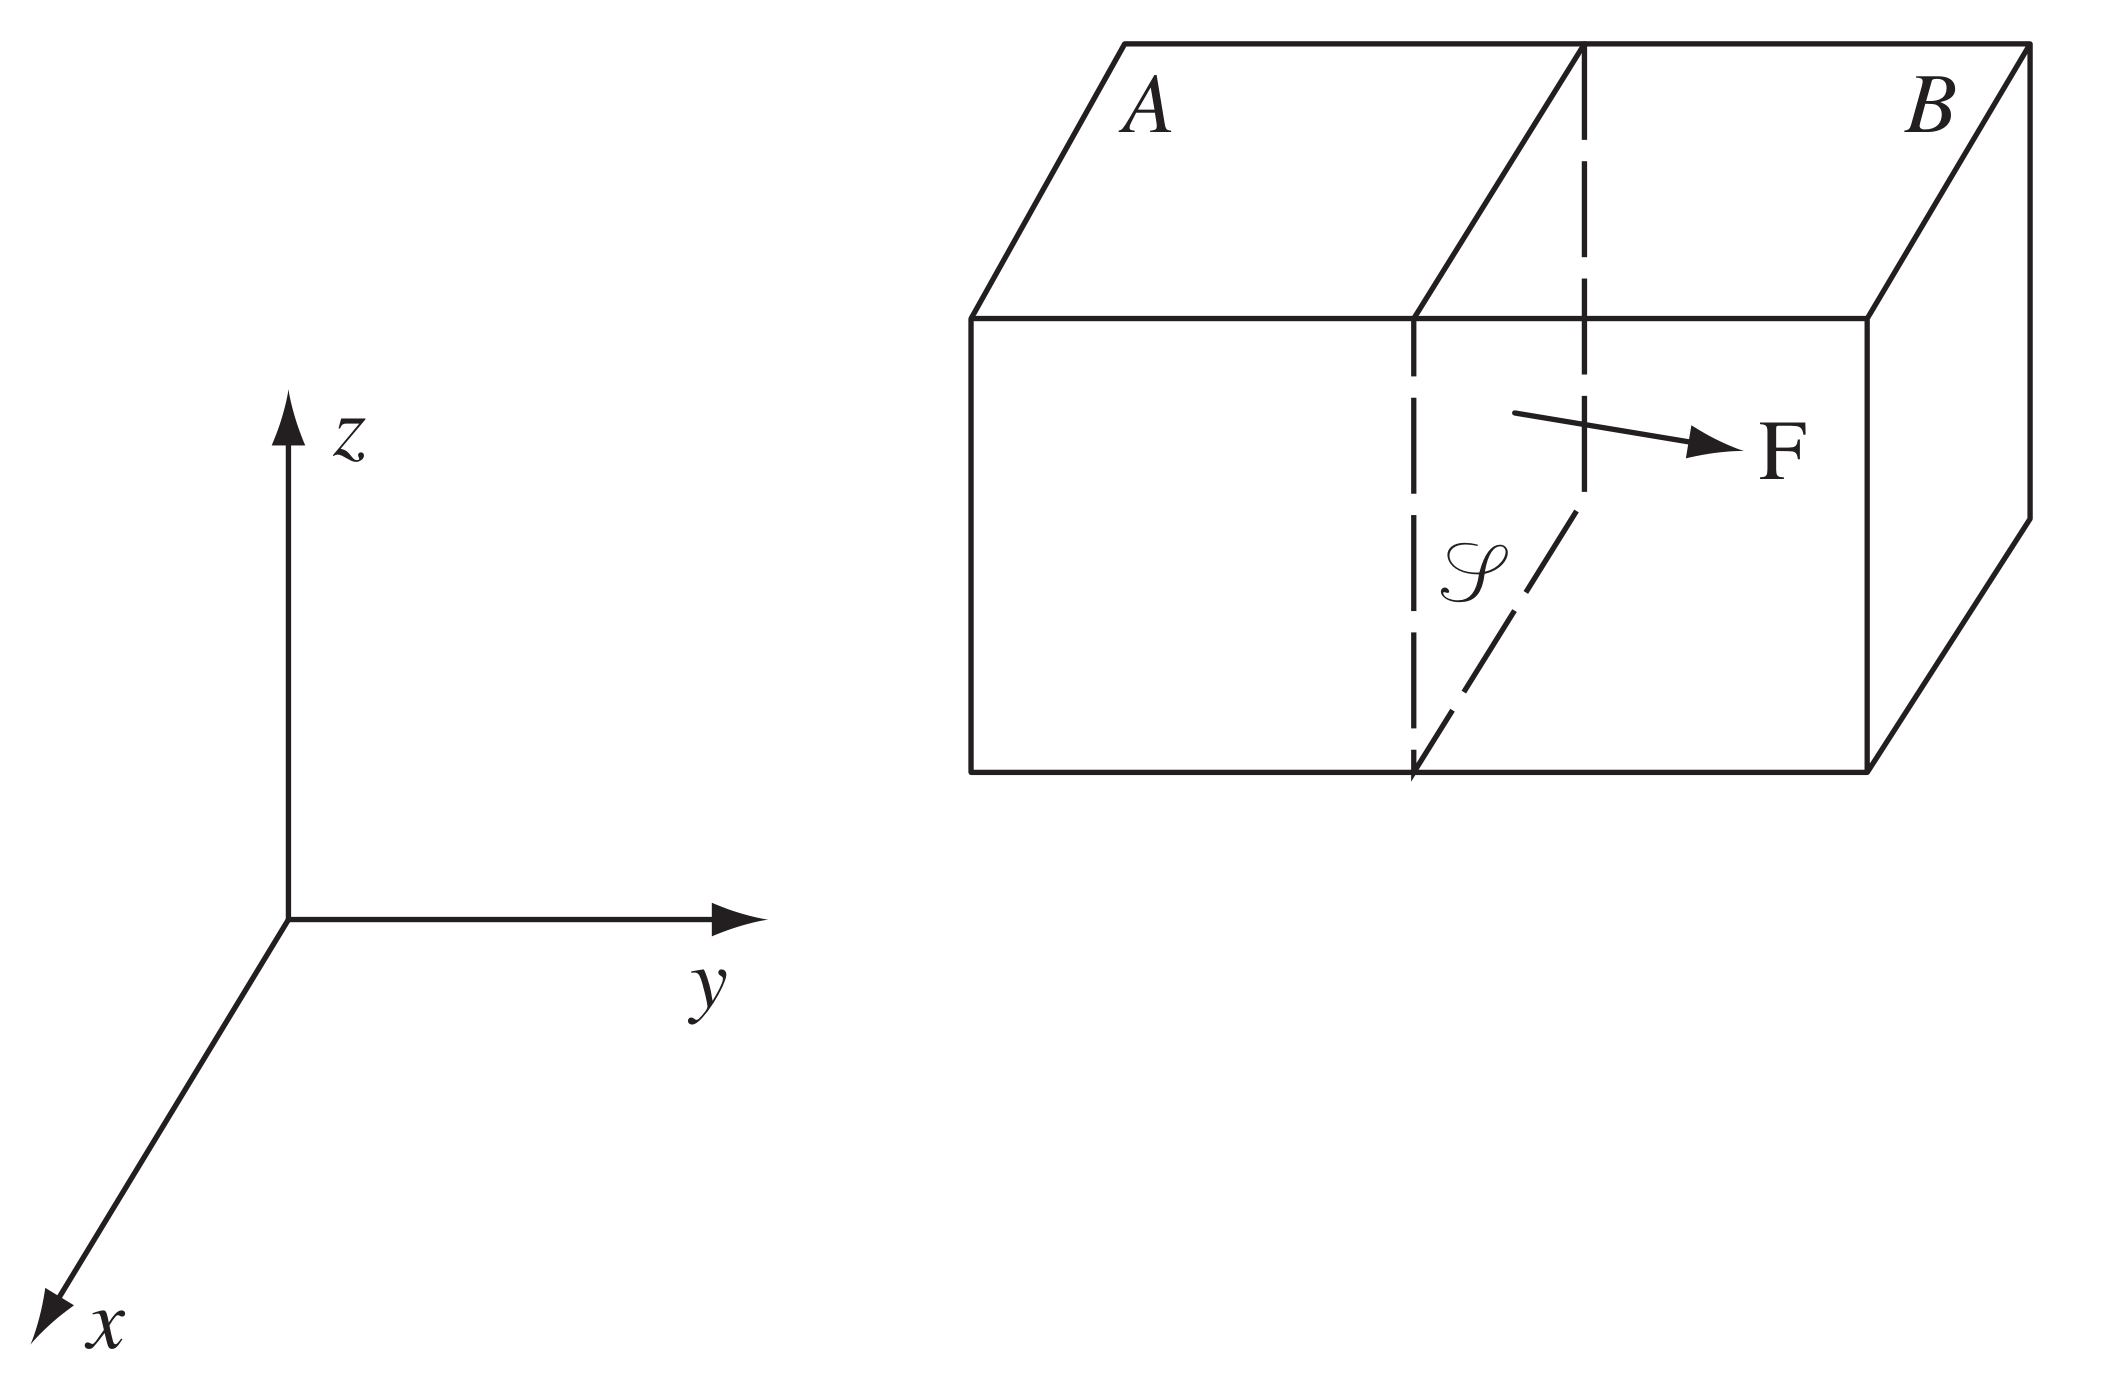
\includegraphics[width=0.6\textwidth]{fig4.6.png}
    \figcaption{\textit{流体元$A$作用于相邻体元$B$的力可能沿任意方向,取决于介质与外力的性质。}}
    \label{fig4.6}
}

图中画出了$A$作用于$B$的力$\bm{F}$(当然,$B$对$A$有等大反向的反作用力)。因为力就是动量的变化率(由于我们在体元速度为零的MCRF中讨论问题,因此牛顿第二定律有效),所以$A$在单位时间内以速度$\bm{F}$向$B$输出动量。当然,取决于相邻体元对它的合外力,体元$B$的动量会发生变化,显然$B$的运动是合外力作用的结果。每个力都向$B$输送动量。从$A$到$B$,穿过界面$\mathscr{S}$,有着速率为$\bm{F}$的动量流量。设$\mathscr{S}$面的面积为$\mathcal{A}$,则通过$\mathscr{S}$面的动量流量为$\bm{F} / \mathcal{A}$。如果$\mathscr{S}$面是等$x^j$面,则流体元$A$的$T^{ij}$等于$F^i / \mathcal{A}$。

$T^{ij}$的物理意义,简单来说,就是相邻流体元之间的力。之前提过,这些力不一定垂直于流体元界面(例如粘性力或其它平行于界面的、为流体提供刚性的力)。如果力\textbf{垂直于}界面,则除非$i = j$,否则$T^{ij} = 0$。(想明白这个结论,后面要用)

\subsection*{MCRF中$T^{\alpha \beta}$的对称性}
现在证明$\mathbf{T}$是对称张量。为此只需要证明它在某一坐标系的分量是对称的,这意味着对任意$\tilde{r}, \tilde{q}$,都有$\mathbf{T} (\tilde{r}, \tilde{q}) = \mathbf{T} (\tilde{q}, \tilde{r})$,也就是说任意坐标系的分量都对称。最简单的坐标系是MCRF。

{
        \centering
        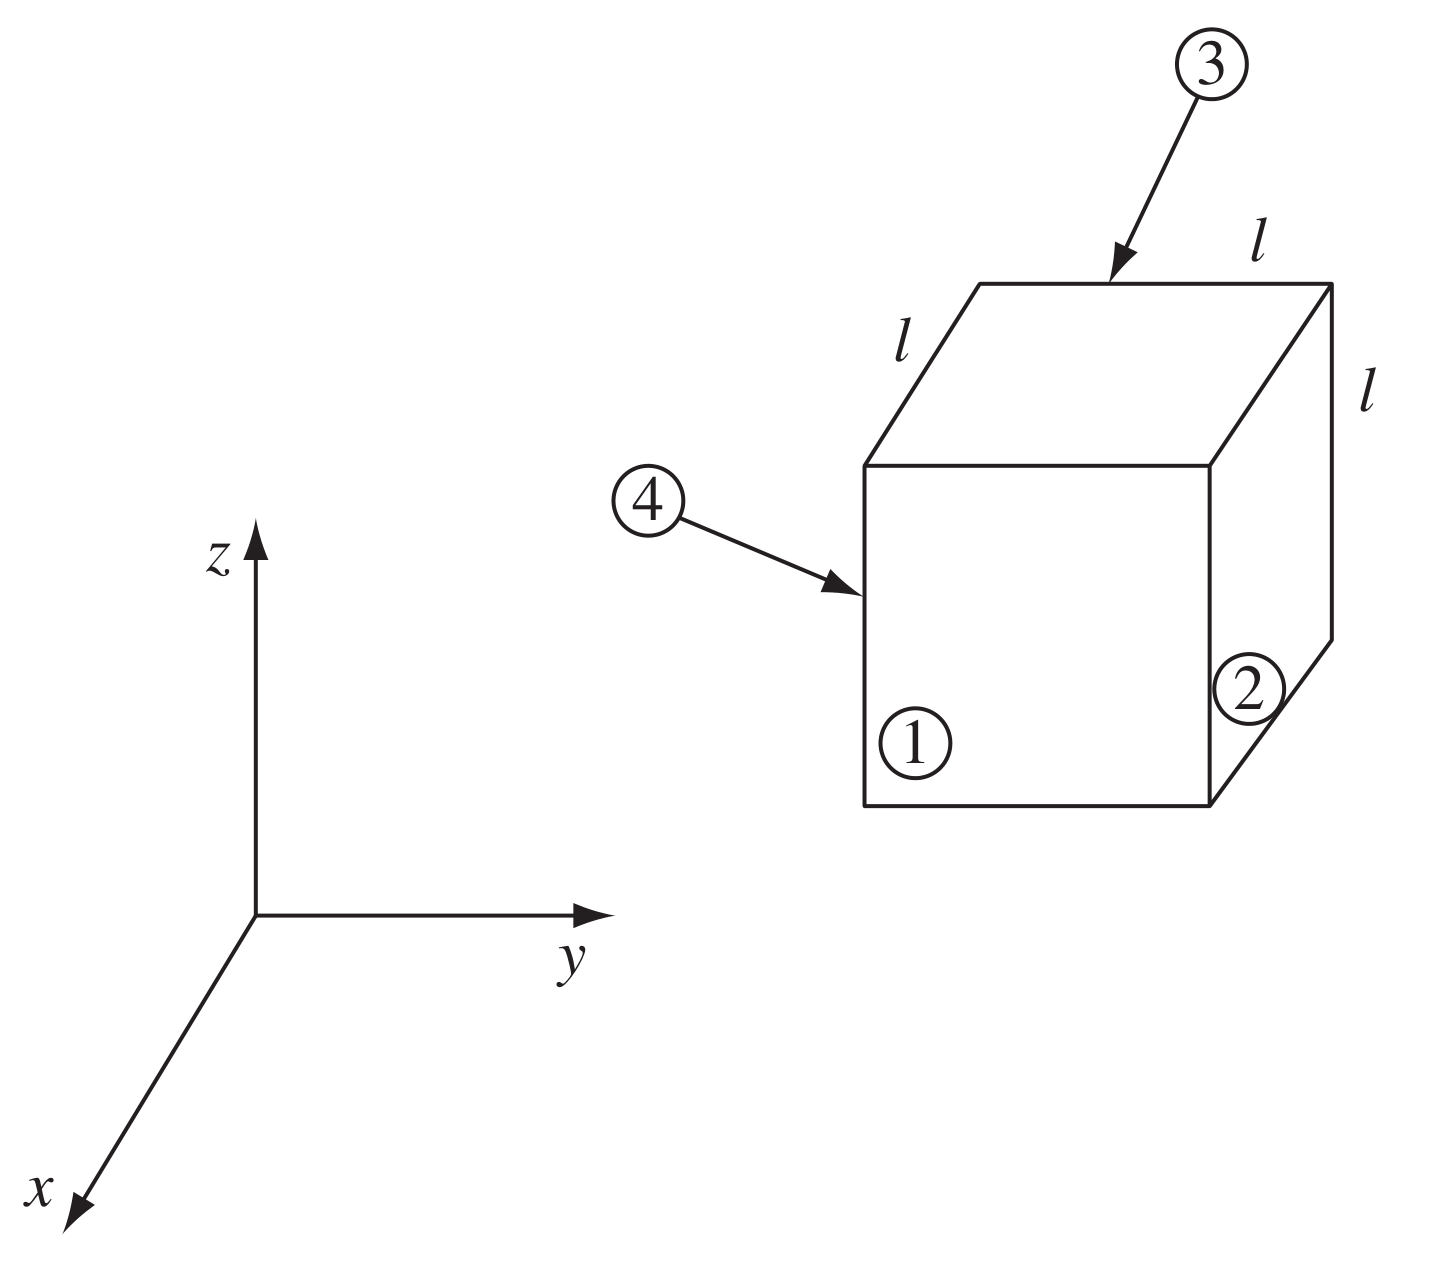
\includegraphics[width=0.6\textwidth]{fig4.7.png}
        \figcaption{\textit{一个流体元。}}
        \label{fig4.7}
}

\begin{enumerate}
    \item $T^{ij}$的对称性。 考虑图\ref{fig4.7},其中画出了边长为$\ell$的立方体流体元。它对与表面(1)(一个$x = \text{constant}$的表面)相邻的体元施加的力等于$F^i_1 = T^{ix} \ell^2$,其中因子$\ell^2$是接触面的面积,由于$\bm{F}$不一定垂直于接触面,因此$i$有$1, 2, 3$三种取值。类似地,该体元通过表面(2)对相邻体元施加的力等于$F_2^i = T^{iy} \ell^2$。(之后会取极限$\ell \to 0$,因此记住流体元很小。)该体元也会对$-x$方向的体元施力,记作$F_3^i$。同理,$F_4^i$是对$-y$方向的力。这个流体元\textbf{所受的}力分别是$-F_1^i, -F_2^i$,等等。

    第一,$F_3^i \approx -F_1^i$,因为体元所受的合力应该随着$\ell \to 0$而趋于零(否则$\ell \to 0$的小质点会有无穷大的加速度)。第二,考虑过体元中心、与$z$轴平行的转轴,计算体元关于该轴的力矩。作用于流体上下表面的力对该力矩无贡献,它们可以忽略。$-\bm{F}_1$对应的力矩为$-(\bm{r} \times \bm{F}_1)^z = -x F_1^y = -\frac{1}{2}\ell T^{yx} \ell^2$,其中将力的作用点近似视为界面中心,$\bm{r} \to (\ell/2, 0, 0)$(注意在那里$y = 0$)。$-\bm{F}_3$对应的力矩\textbf{同样}是$-\frac{1}{2} \ell^3 T^{yx}$。$-\bm{F}_2$的力矩是$-(\bm{r} \times \bm{F}_2)^z = +yF_2^x = \frac{1}{2} \ell T^{xy} \ell^2$. 同理,$-\bm{F}_4$的力矩是$\frac{1}{2} \ell^3 T^{xy}$。因此,总力矩为
    \begin{equation}
        \tau_z = \ell^3 (T^{xy} - T^{yx}).
    \label{equ4.27}
    \end{equation}
    流体元关于$z$轴的转动惯量正比于其质量乘以$\ell^2$,即:
    \[
        I = \alpha \rho \ell^5,
    \]
    其中$\alpha$是某个常数,$\rho$是密度(这里无论是总能量还是静质量都无所谓)。因此角加速度为
    \begin{equation}
        \ddot{\theta} = \frac{\tau}{I} = \frac{T^{xy} - T^{yx}}{\alpha \rho \ell^2}.
    \label{equ4.28}
    \end{equation}
    因为$\alpha$是常数,$\rho$、$T^{xy}\text{与}T^{yx}$与体元的大小无关,所以在$\ell \to 0$的极限下,为了避免无穷大的角加速度,必须
    \[
        T^{xy} = T^{yx}.
    \]
    因此,根据流体元没有绕内部流体旋转、越小的流体并非旋转越快,我们得出结论,应力总是\textbf{对称的}:
    \begin{equation}    
        T^{ij} = T^{ji}.
    \label{equ4.29}
    \end{equation}  
    推导过程并未涉及物质的特殊性质,因此该结论对固体、流体都适用。在狭义相对论中,牛顿理论也能用,牛顿理论中$T^{ij}$是三维$\binom{2}{0}$张量——应力张量的分量,材料工程师对它很熟悉,它的名字保留作为相对论推广量$\mathbf{T}$的一部分。
    \item 动量密度等于能量流的证明。这比上一条简单多了。能量流是能量密度乘以能量流动的速率,由于能量与质量相同,因此能量流等于质量密度乘以它流动的速率;换句话说,就是动量密度,因此$T^{0i} = T^{i0}$.    
\end{enumerate}


\subsection*{能量-动量守恒}
由于$\mathbf{T}$表示流体的能量、动量,因此可以用它表示能量动量守恒定律,实际上相应的形式超级简单。考虑图\ref{fig4.8}中的管状体元,只考虑其横截面(图中省略了$z$轴)。

{
    \centering
    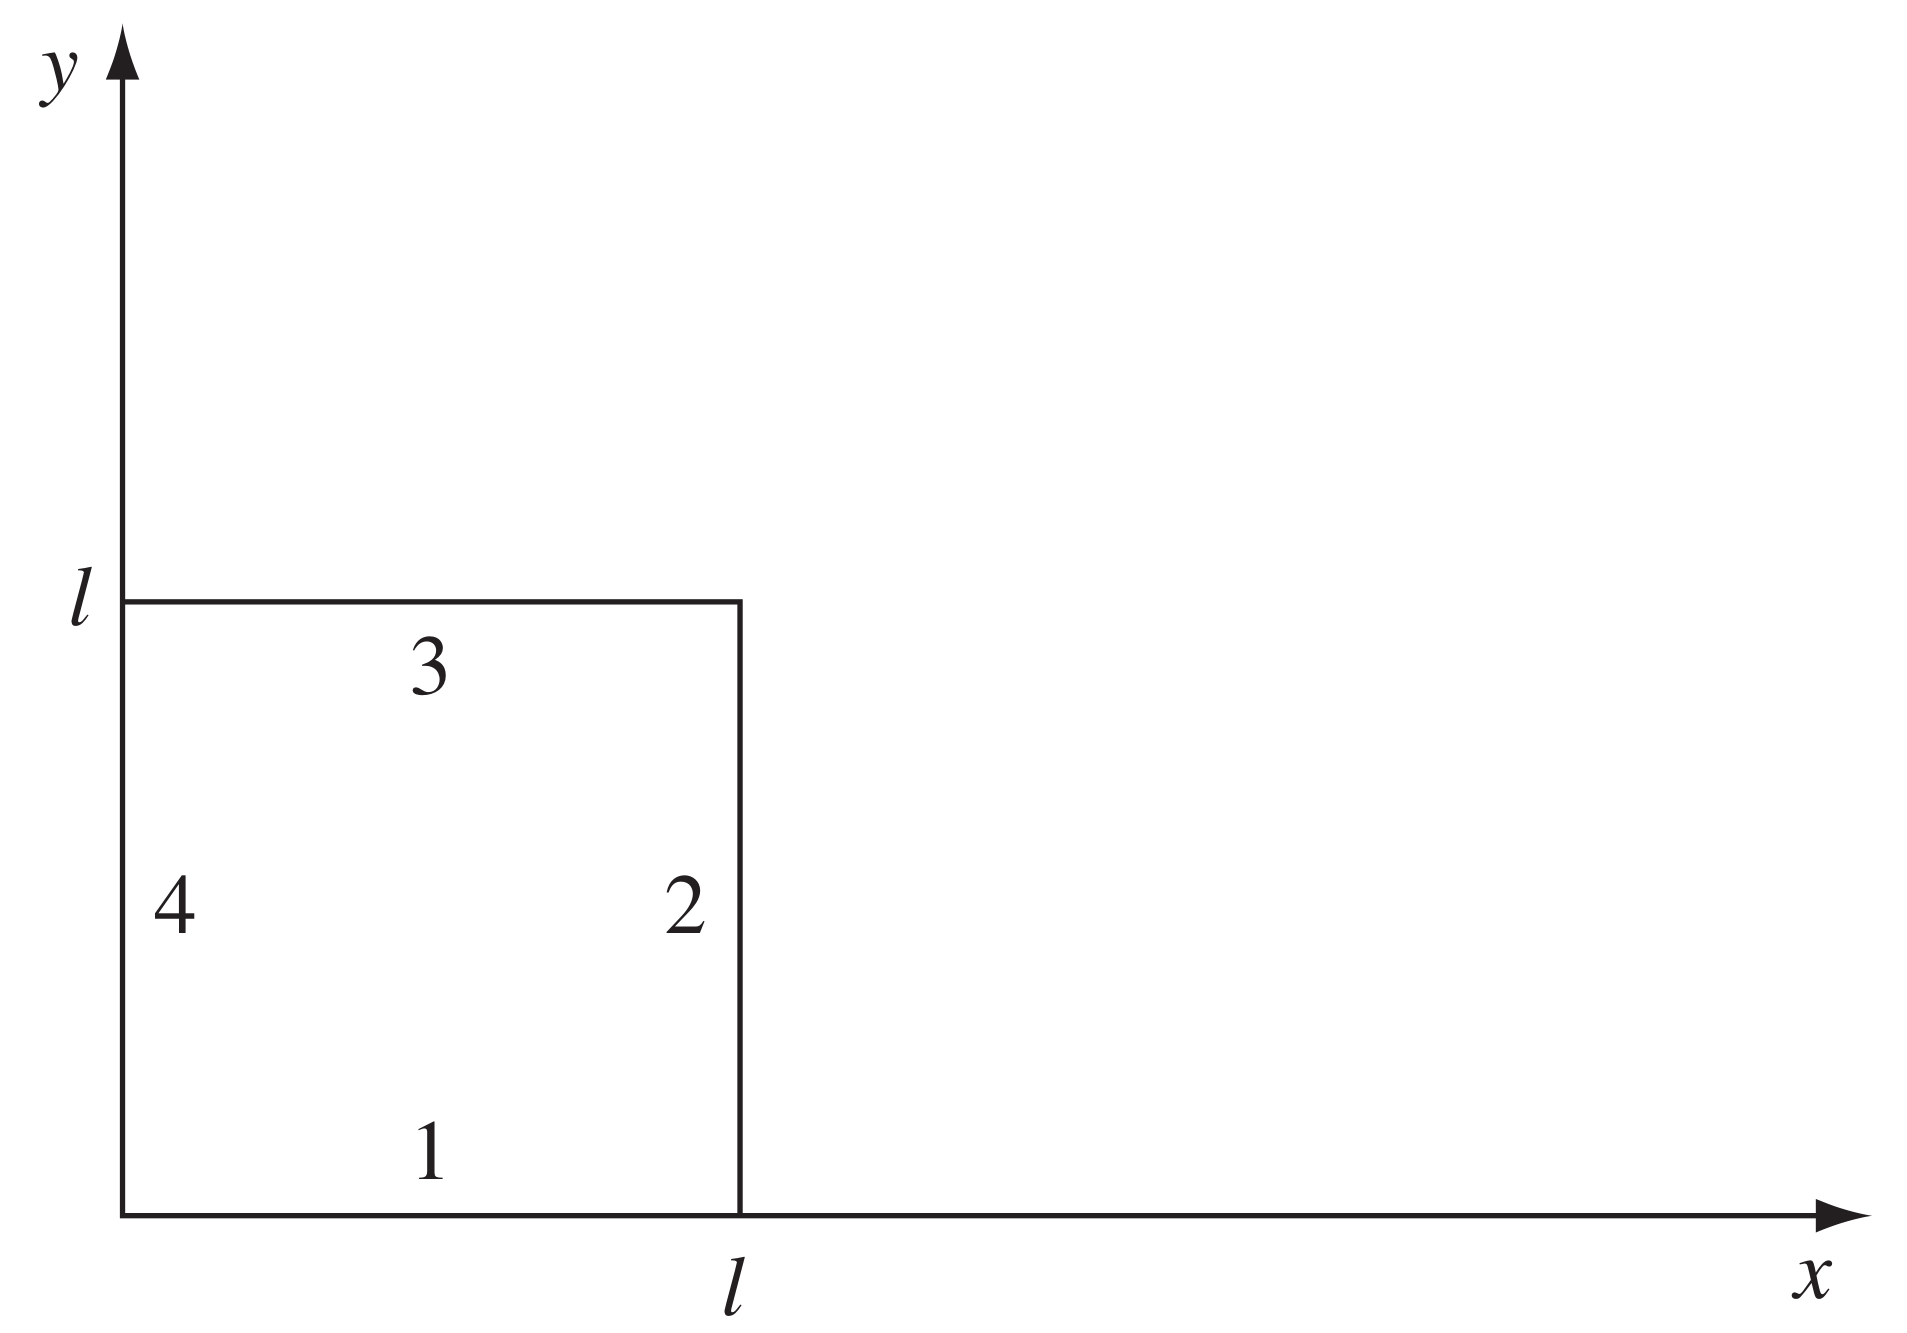
\includegraphics[width=0.6\textwidth]{fig4.8.png}
    \figcaption{\textit{一个管状流体元的$z = \text{constant}$横截面。}}
    \label{fig4.8}
}

能量可以从体元的各个表面流进流出。能量通过表面(4)流入体元的速率为$\ell^2 T^{0x} (x = 0)$;通过表面(2)流入体元的速率为$-\ell^2 T^{0x} (x = a)$,注意其中的负号,因为$T^{0x}$表示能量沿正$x$方向的流动,它在(2)处取值的方向为流出体元。同理,从$y$方向流入体元的能量为$\ell^2 T^{0y} (y = 0) - \ell^2 T^{0y} (y = \ell)$。根据能量守恒,它们之和等于流体元能量的增长率$\partial(T^{00} \ell^3) / \partial t$,由此可得
\begin{align}
    \frac{\partial}{\partial t} (\ell^3 T^{00}) = \ell^2 \Big[& T^{0x}|_{x = 0} - T^{0x}|_{x = \ell} \notag \\
    & + T^{0y}|_{y = 0} - T^{0y}|_{y = \ell} + T^{0z}|_{z = 0} - T^{0z}|_{z = \ell} \Big]. \label{equ4.30}
\end{align}
两边除以$\ell^3$并取极限$\ell \to 0$,并注意到
\begin{equation}
\lim_{\ell \to 0} \dfrac{T^{0x}|_{x = 0} - T^{0x}|_{x = \ell}}{\ell} \equiv -\frac{\partial}{\partial x} T^{0x},
\label{equ4.32}
\end{equation}
于是\eqref{equ4.30}式化为:
\begin{equation}
    \frac{\partial}{\partial t} T^{00} = -\frac{\partial}{\partial x} T^{0x} - \frac{\partial}{\partial y} T^{0y} - \frac{\partial}{\partial z} T^{0z}.
\label{equ4.31}
\end{equation}

\eqref{equ4.31}式可以写为
\begin{align}
    T\indices{^{00}_{, 0}} &+ T\indices{^{0x}_{,x}} + T\indices{^{0y}_{,y}} + T\indices{^{0z}_{,z}} = 0 \notag \\
\intertext{或者}
    T\indices{^{0\alpha}_{, \alpha}} &= 0. \label{equ4.33}
\end{align}
这就是能量守恒的表达式。

动量守恒的情形同理。利用相似的推导过程,可以证明$T\indices{^{i \alpha}_{, \alpha}} = 0$,因此一般的守恒定律可以表述为
\begin{shaded}
\begin{equation}
    T\indices{^{\alpha \beta}_{, \beta}} = 0.
\label{equ4.34}
\end{equation}
\end{shaded}
这对SR中的任何系统都成立。注意,上式就是四维散度,因而与高斯定理(守恒律的积分形式)有关,后面会进行相关讨论。

\subsection*{粒子守恒}
在流体流动的过程中,流体元的粒子数可能会改变,但是流体总体的粒子数不变。在图\ref{fig4.8}中,流体元当中粒子数的变化是由于粒子从边界面流入流出引起的,变化率等于流入或流出的净流量。这种粒子数守恒可以通过与\eqref{equ4.34}式类似的方式推导出来,这里直接给出结果:
\[
    \frac{\partial}{\partial t} N^0 = -\frac{\partial}{\partial x} N^x - \frac{\partial}{\partial y} N^y - \frac{\partial}{\partial z} N^z,
\]
或者写为
\begin{shaded}
\begin{equation}
    N\indices{^\alpha_{, \alpha}}  = (n U^\alpha)_{, \alpha} = 0.
\label{equ4.35}
\end{equation}
\end{shaded}
我们只考虑这种服从粒子数守恒的流体。这是个很弱的限制,因为粒子数密度$n$几乎总可以取为重子的,重子绝大部分情况下守恒。

对于不熟悉高能物理的人,“重子(baryon)”的概念比较陌生,它是物理学中一类大质量粒子的统称,最常见的重子是中子和质子。其它重子不稳定,在日常物理学的地位不如前两者重要,但是它们会衰变成质子和中子,保证了重子数守恒,但不能保证静质量、特定种类的重子数。尽管理论物理学家认为重子数可能不守恒——例如,强、弱和电磁相互作用的“大统一理论”认为质子具有有限长的寿命,黑洞的坍缩与之后的蒸发(见\ref{chap11}章)不满足重子数守恒——但是这些现象目前并未观测到,而且在大部分情况下都不重要。


\section{理想流体}
\label{sec4.6}

\section{对于广义相对论的重要性}
\label{sec4.7}

\section{高斯定律}
\label{sec4.8}

\section{扩展阅读}
\label{sec4.9}

\section{习题}
\label{sec4.10}

\chapter{曲率的序言}
\label{chap5}

\section{引力与曲率的关系}
\label{sec5.1}
目前我们都是在狭义相对论(SR)中讨论问题。力在SR当中的地位很重要,但是前面从来没有直接研究引力。SR的一个重要基础是存在覆盖整个时空的惯性系:全体时空可以由一个坐标系描述,这个系的所有坐标点都相对于原点静止,所有的坐标钟与原点的钟走时率相同。从这个基本假设可以导出时间间隔$\Delta s^2$的概念,它给物理事件赋予了具有不变性的几何意义。例如,两事件之间的类时间隔是经过这两个时件的钟所走过的时间;类空间隔是在这两个事件同时的坐标系当中的空间距离。

\section{极坐标系的张量代数}
\label{sec5.2}
考虑欧几里得平面。直角坐标$\{x, y\}$,极坐标$\{r, \theta\}$之间的关系为:
\begin{equation}
    \left.
    \begin{split}
    r &= (x^2 + y^2)^{1/2}, \quad x = r \cos \theta, \\
    \theta &= \Arctan (y / x), \quad y = r \sin \theta.
    \end{split}
    \right\}
\label{equ5.3}
\end{equation}

由直角坐标的微小增量$\Delta x, \Delta y$造成的$\Delta r, \Delta \theta$为
\begin{equation}
\left.
\begin{split}
    \Delta r &= \frac{x}{r} \Delta x + \frac{y}{r} \Delta y = \cos \theta \Delta x + \sin \theta \Delta y, \\
    \Delta \theta &= -\frac{y}{r^2} \Delta x + \frac{x}{r^2} \Delta y = -\frac{1}{r} \sin \theta \Delta x + \frac{1}{r} \cos \theta \Delta y,
\end{split}
\right\}
\label{equ5.4}
\end{equation}
上式到一阶小量都成立。

也可以使用其它坐标系。记一般的坐标系为$\{ \xi, \eta \}$:
\begin{equation}
\left.
\begin{split}
    \xi &= \xi (x, y), \quad \Delta \xi = \frac{\partial \xi}{\partial x} \Delta x + \frac{\partial \xi}{\partial y} \Delta y, \\
    \eta &= \eta (x, y), \quad \Delta \eta = \frac{\partial \eta}{\partial x} \Delta x + \frac{\partial \eta}{\partial y} \Delta y.
\end{split}
\right\}
\label{equ5.5}
\end{equation}
为了保证$(\xi, \eta)$是个好坐标系,任意两个不同的点$(x_1, y_1)$和$(x_2, y_2)$应该对应不同的$(\xi_1, \eta_1)$与$(\xi_2, \eta_2)$(通过\eqref{equ5.5}式对应)。例如,按$\xi = x, \eta = 1$定义的坐标系不是好坐标系,因为不同的两点$(x = 1, y = 2)$和$(x = 1, y = 3)$都对应$(\xi = 1, \eta = 1)$。数学上,这要求如果方程\eqref{equ5.5}中的$\Delta \xi = \Delta \eta = 0$,则必须对应相同的点,即$\Delta x = \Delta y = 0$. 这意味着\eqref{equ5.5}式的行列式非零:
\begin{equation}
    \det \begin{pmatrix}
        \partial \xi / \partial x & \partial \xi / \partial y \\
        \partial \eta / \partial x & \partial \eta / \partial y
    \end{pmatrix} 
    \neq 0.
\label{equ5.6}
\end{equation}
这个行列式称为坐标系变换\eqref{equ5.5}式的\textit{Jacobian}(\textit{雅可比行列式})。如果Jacobian在某一点为零,则称坐标变换在该点具有\textit{奇性 (singular)}。

\subsection*{向量与1形式}
向量的旧的定义是在\textit{任意}坐标变换下与位移的变换方式相同的量。也就是说,向量$\Delta \vec{r}$可以表示为\footnote{欧几里得空间的向量用箭头标记,其分量指标(1, 2)用希腊字母表示,求和对所有指标进行。}位移$(\Delta x, \Delta y)$,或者在极坐标系表示为$(\Delta r, \Delta \theta)$,或者在一般坐标系中为$(\Delta \xi, \Delta \eta)$. 根据\eqref{equ5.5}式,对于微小的$(\Delta x, \Delta y)$有:
\begin{equation}
    \begin{pmatrix}
        \Delta \xi \\ \Delta \eta
    \end{pmatrix}
    =
    \begin{pmatrix}
        \partial \xi / \partial x & \partial \xi / \partial y \\
        \partial \eta / \partial x & \partial \eta / \partial y 
    \end{pmatrix}
    \begin{pmatrix}
        \Delta x \\ \Delta y 
    \end{pmatrix}.
\label{equ5.7}
\end{equation}
定义变换矩阵
\begin{equation}
    (\Lambda\indices{^{\alpha'}_{\beta}}) = 
    \begin{pmatrix}
        \partial \xi / \partial x & \partial \xi / \partial y \\
        \partial \eta / \partial x & \partial \eta / \partial y 
    \end{pmatrix},
\label{equ5.8}
\end{equation}
则可以将任意向量$\vec{V}$的分量的变换规律写成与SR相同的形式:
\begin{equation}
    V^{\alpha'} = \Lambda\indices{^{\alpha'}_{\beta}} V^\beta,
\label{equ5.9}
\end{equation}
其中不带撇的指标代表$(x, y)$,带撇指标表示$(\xi, \eta)$,指标取$1, 2$. 向量可以定义为分量按照\eqref{equ5.9}式变换的这样的量。不过,存在一种更加复杂而自然的、现代的定义方式,下面进行介绍。

考虑平面上的标量场$\phi$。给定坐标系$(\xi, \eta)$就能计算偏导数$\partial \phi / \partial \xi$和$\partial \phi / \partial \eta$. \textit{定义}1形式$\trd \phi$为(在坐标系$(\xi, \eta)$中)具有如下分量的几何对象:
\begin{equation}
    \trd \phi \to (\partial \phi / \partial \xi, \partial \phi / \partial \eta).
\label{equ5.10}
\end{equation}
这是1形式的一般定义,每个标量场都定义了一个1形式。1形式分量的变换规律可以通过链式法则(chain rule)导出:
\begin{equation}
    \frac{\partial \phi}{\partial \xi} = \frac{\partial x}{\partial \xi} \frac{\partial \phi}{\partial x} + \frac{\partial y}{\partial \xi} \frac{\partial \phi}{\partial y},
\label{equ5.11}
\end{equation}
$\partial \phi / \partial \eta$同理。用\textit{行向量}可以方便地用矩阵形式表示:
\begin{equation}
\begin{pmatrix}
    \partial \phi / \partial \xi & \partial \phi / \partial \eta
\end{pmatrix}
=
\begin{pmatrix}
    \partial \phi / \partial x & \partial \phi / \partial y
\end{pmatrix}
\begin{pmatrix}
    \partial x / \partial \xi & \partial x / \partial \eta \\
    \partial y / \partial \xi & \partial y / \partial \eta
\end{pmatrix},
\label{equ5.12}
\end{equation}

1形式的变换矩阵可类比\eqref{equ5.8}式定义为一组$(x, y)$坐标关于$(\xi, \eta)$坐标的偏导数:
\begin{equation}
    ( \Lambda\indices{^\alpha_{\beta'}} ) = 
    \begin{pmatrix}
        \partial x / \partial \xi & \partial x / \partial \eta \\
        \partial y / \partial \xi & \partial y / \partial \eta
    \end{pmatrix}
\label{equ5.13}
\end{equation}
这样,\eqref{equ5.12}式就可以写成分量求和的形式:
\begin{equation}
    (\trd \phi)_{\beta'} = \Lambda\indices{^\alpha_{\beta'}} (\trd \phi)_\alpha.
\label{equ5.14}
\end{equation}
注意,上式的求和是对变换矩阵的\textit{第一个}分量进行的,这对应于行向量左乘矩阵。

值得一提的是,SR从来没考虑过行向量,因为Lorentz变换矩阵是个简单的对称矩阵。不过即使是上面的简单情况也要用到行向量。当张量的指标多于两个时,矩阵表示就非常累赘。GR需要处理四个甚至五个指标的张量,因此后面一般用代数形式(如\eqref{equ5.14}式)表示变换,后面就不再使用矩阵表示了。

本节已经看到,在现代观点之下,张量代数的基础是1形式的定义。它比旧定义更加自然,旧定义首先定义了\textit{单个}向量$(\Delta x, \Delta y)$,其它向量类比它定义。而现代定义利用偏导数定义了\textit{一类}1形式,1形式分量的变换规律自然地随之导出。

向量定义为将1形式映射为实数的线性函数。这个定义的具体含义在下一小节讲述。先来说明与SR形式的相似性,向量的变换规律为$\eqref{equ5.9}$式,有趣的是变换矩阵$(\Lambda\indices{^{\alpha'}_\beta})$和$( \Lambda\indices{^\alpha_{\beta'}} )$互逆。它们相乘得到:
\begin{align}
    \begin{pmatrix}
        \partial \xi / \partial x & \partial \xi / \partial y \\
        \partial \eta / \partial x & \partial \eta / \partial y 
    \end{pmatrix}
    \begin{pmatrix}
        \partial x / \partial \xi & \partial x / \partial \eta \\
        \partial y / \partial \xi & \partial y / \partial \eta
    \end{pmatrix} \notag \\
    =
    \begin{pmatrix}
        \dfrac{\partial \xi}{\partial x} \dfrac{\partial x}{\partial \xi} + \dfrac{\partial \xi}{\partial y} \dfrac{\partial y}{\partial \xi} & \dfrac{\partial \xi}{\partial x} \dfrac{\partial x}{\partial \eta} + \dfrac{\partial \xi}{\partial y} \dfrac{\partial y}{\partial \eta}  \\
        \dfrac{\partial \eta}{\partial x} \dfrac{\partial x}{\partial \xi} + \dfrac{\partial \eta}{\partial y} \dfrac{\partial y}{\partial \xi} & \dfrac{\partial \eta}{\partial x} \dfrac{\partial x}{\partial \eta} + \dfrac{\partial \eta}{\partial y} \dfrac{\partial y}{\partial \eta}
    \end{pmatrix}.
\label{equ5.15}
\end{align}
利用链式法则与偏导数的定义可以算出结果为
\begin{equation}
    \begin{pmatrix}
        \partial \xi / \partial \xi & \partial \xi / \partial \eta \\
        \partial \eta / \partial \xi & \partial \eta / \partial \eta
    \end{pmatrix}
    = 
    \begin{pmatrix}
        1 & 0 \\
        0 & 1
    \end{pmatrix}。
\label{equ5.16}
\end{equation}

\subsection*{曲线与向量}
通常所说的曲线是平面上一系列连续的点,我们把它称作\textit{路径 (path)},而把曲线专指参数化的路径。这也是现代数学的做法,将\textit{曲线 (curve)}定义为从实数区间到平面路径的映射。这意味着曲线是每一点都对应一个实数的路径,实数称为参数(parameter),记作$s$。每一点的坐标表示为参数$s$的函数就定义了平面上的一条曲线:
\begin{shaded}
\begin{equation}
    \text{曲线:} \{ \xi = f(s), \eta = g(s), \quad a \le s \le b \}
\label{equ5.17}
\end{equation}
\end{shaded}
将参数改变为$s' = s'(s)$(新参数是旧参数的函数,点不变),则有
\begin{equation}
    \text{曲线:} \{ \xi = f'(s'), \eta = g'(s'), \quad a' \le s' \le b' \},
\label{equ5.18}
\end{equation}
其中$f', g'$是\textit{新的}函数,而$a' = s'(a), b' = s'(b)$. 上式在数学上是一条\textit{新的}曲线,尽管它的\textit{像 (image)}(所经过的平面上的点)与原来相同。因此同一路径对应无数条曲线。

标量场$\phi$沿曲线的导数是$\rd \phi / \rd s$,依赖于$s$,因此变换参数,导数也随之变换。可以将导数写为
\begin{equation}
    \frac{\rd \phi}{\rd s} = \langle \trd \phi, \vec{V} \rangle,
\label{equ5.19}
\end{equation}
其中$\vec{V}$是分量为$(\rd \xi / \rd s, \rd \eta / \rd s)$的向量,这个向量只与曲线有关,而$\trd \phi$只依赖于$\phi$. 因此$\vec{V}$是与曲线特征有关的向量,称之为\textit{切向量 (tangent vector)}。(见图\ref{fig5.4},显然它与曲线相切) \ \sout{画外音:哪里显然了……}

所以,向量可以看作是给定$\phi$而产生$\rd \phi / \rd s$的东西。这就引出了最现代的观点,曲线的切向量应该\textit{称为} $\rd / \rd s$。有些相对论文献偶尔使用这一符号。不过我们把它记作$\vec{V}$,知道它的分量是$(\rd \xi / \rd s, \rd \eta / \rd s)$就好了。注意,平面上的一条路径上的任一点都有着无数切向量,它们的方向相同而长度不同,它们可以视为\textit{不同}曲线(在一点邻域中的参数化不同)的切向量。曲线是给定了参数的路径,因此曲线的切向量\textit{唯一}。此外,即使两条曲线在某一点的切向量相等,它们在其它点也可以不同,根据Taylor展开式$\xi (s + 1) \approx \xi (s) + \rd \xi / \rd s$可见,$\vec{V} (s)$近似沿曲线从$s$到$s + 1$延展。

{
    \centering
    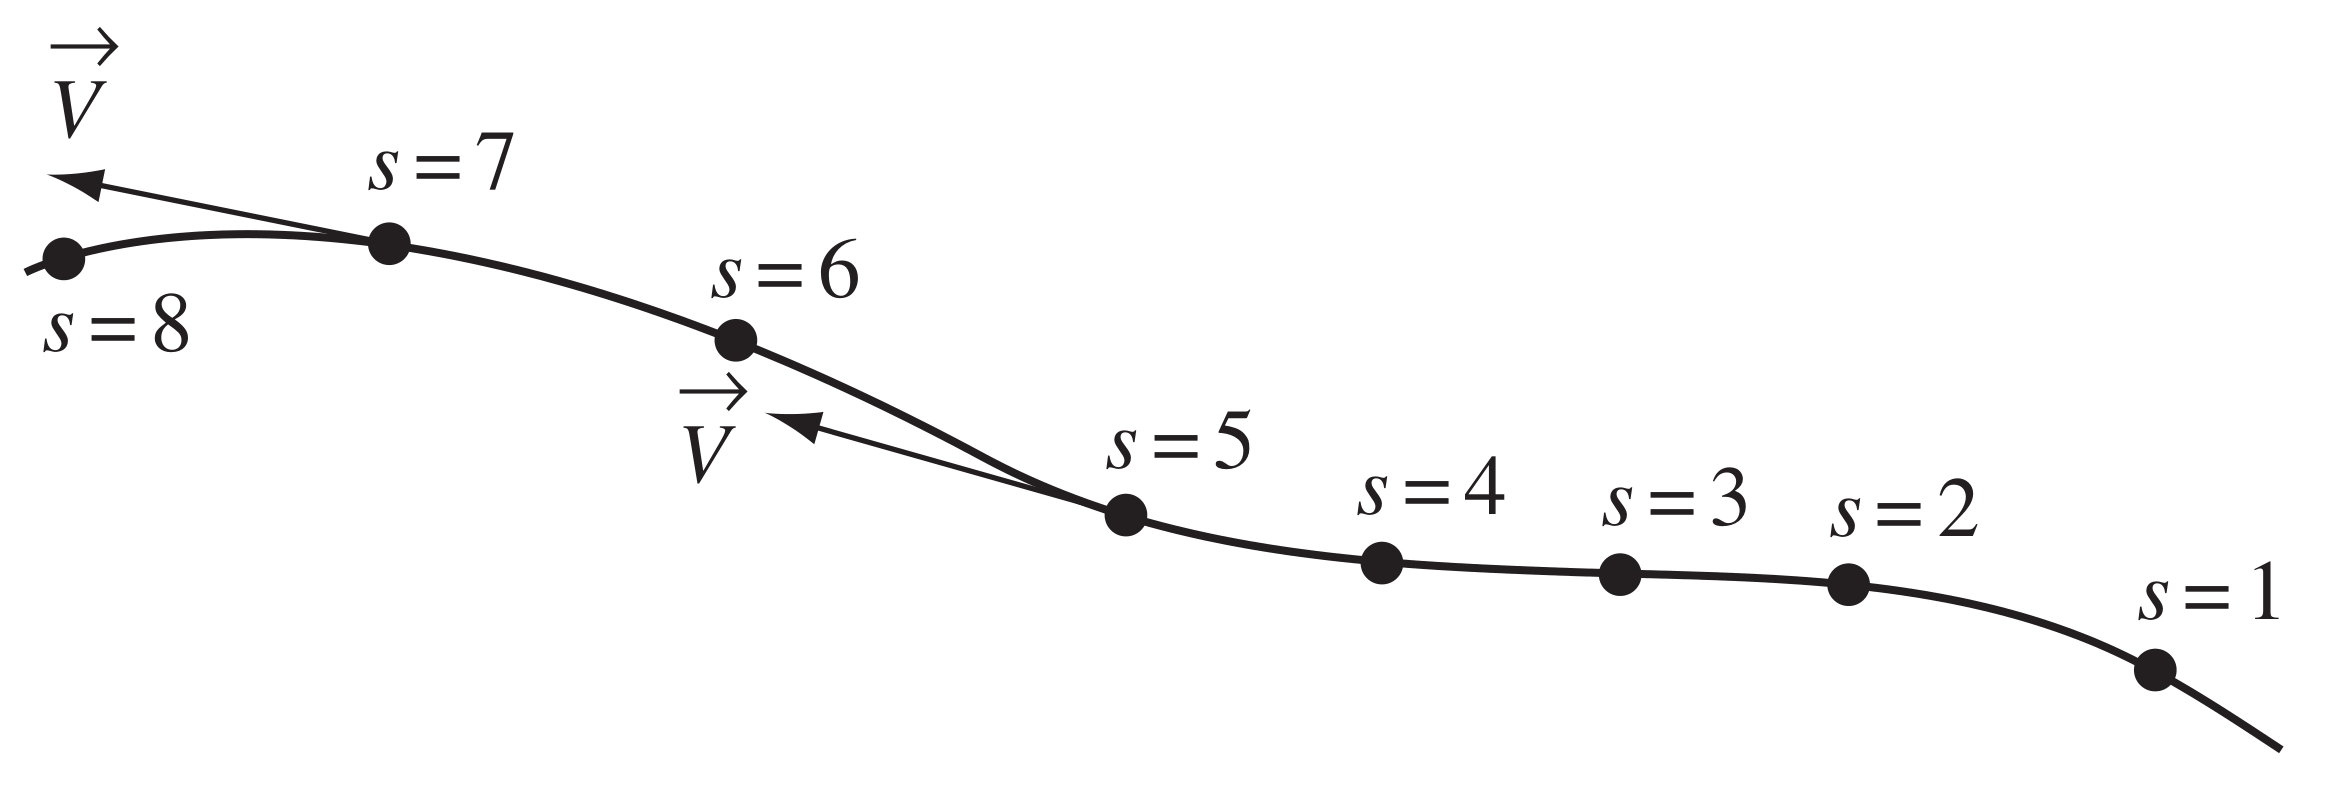
\includegraphics[width=0.6\textwidth]{fig5.4.png}
    \figcaption{\textit{一条曲线,曲线的参数,以及曲线的切向量}}
    \label{fig5.4}
}

注意$s$在坐标变换下不变(它的定义和坐标系无关),而$\vec{V}$的分量变化,因此根据链式法则可得
\begin{equation}
    \begin{pmatrix}
        \rd \xi / \rd s \\
        \rd \eta / \rd s
    \end{pmatrix}
    =
    \begin{pmatrix}
        \partial \xi / \partial x & \partial \xi / \partial y \\
        \partial \eta / \partial x & \partial \eta / \partial y
    \end{pmatrix}
    \begin{pmatrix}
        \rd x / \rd s \\
        \rd y / \rd s
    \end{pmatrix}.
\label{equ5.20}
\end{equation}
这与前面的向量变换律\eqref{equ5.7}式相同。

总结一下现代观点,向量是与某条曲线相切、将$\trd \phi$映射为$\rd \phi / \rd s$的线性函数。这样,下面就能更进一步地研究极坐标系。

\subsection*{极坐标系的1形式基与向量基}
显然,坐标基向量的变换规律为:
\begin{equation*}
    \vec{e}_{\alpha'} = \Lambda\indices{^\beta_{\alpha'}} \vec{e}_\beta,
\end{equation*}
在极坐标下:
\begin{align}
    \vec{e}_r &= \Lambda\indices{^x_r} \Ve_x + \Lambda\indices{^y_r} \Ve_y \label{equ5.21} \\
    &= \frac{\partial x}{\partial r} \Ve_x + \frac{\partial y}{\partial r} \Ve_y \notag \\
    &= \cos \theta \Ve_x + \sin \theta \Ve_y, \label{equ5.22}
\end{align}
类似有
\begin{align}
    \Ve_\theta &= \frac{\partial x}{\partial \theta} \Ve_x + \frac{\partial y}{\partial \theta} \Ve_y \notag \\
    &= -r \sin \theta \Ve_x + r \cos \theta \Ve_y, \label{equ5.23}
\end{align}
注意,上式已经利用了
\begin{equation}
    \Lambda\indices{^x_r} = \frac{\partial x}{\partial r}.
\label{equ5.24}
\end{equation}
类似地,“反向”变换的矩阵元为
\begin{equation}
    \Lambda\indices{^r_x} = \frac{\partial r}{\partial x}.
\label{equ5.25}
\end{equation}
这个变换矩阵十分简单:矩阵指标的上下顺序对应到求导的上下关系就好了。

1形式基的关系可类似求出:
\begin{align}
    \trd \theta &= \frac{\partial \theta}{\partial x} \trd x + \frac{\partial \theta}{\partial y} \trd y, \notag \\
    &= -\frac{1}{r} \sin \theta \trd x + \frac{1}{r} \cos \theta \trd y. \label{equ5.26}
\end{align}
(注意上式与普通的微积分运算\eqref{equ5.4}式相似)。同样可得
\begin{equation}
    \trd r = \cos \theta \trd x + \sin \theta \trd y.
\label{equ5.27}
\end{equation}
根据以上内容可以画出不同点的基(图\ref{fig5.5})。容易画出基向量,1形式基可以画出$\trd r$和$\trd \theta$的等$r$、等$\theta$面辅助进行,不同位置的面的指向不同。

{
    \centering
    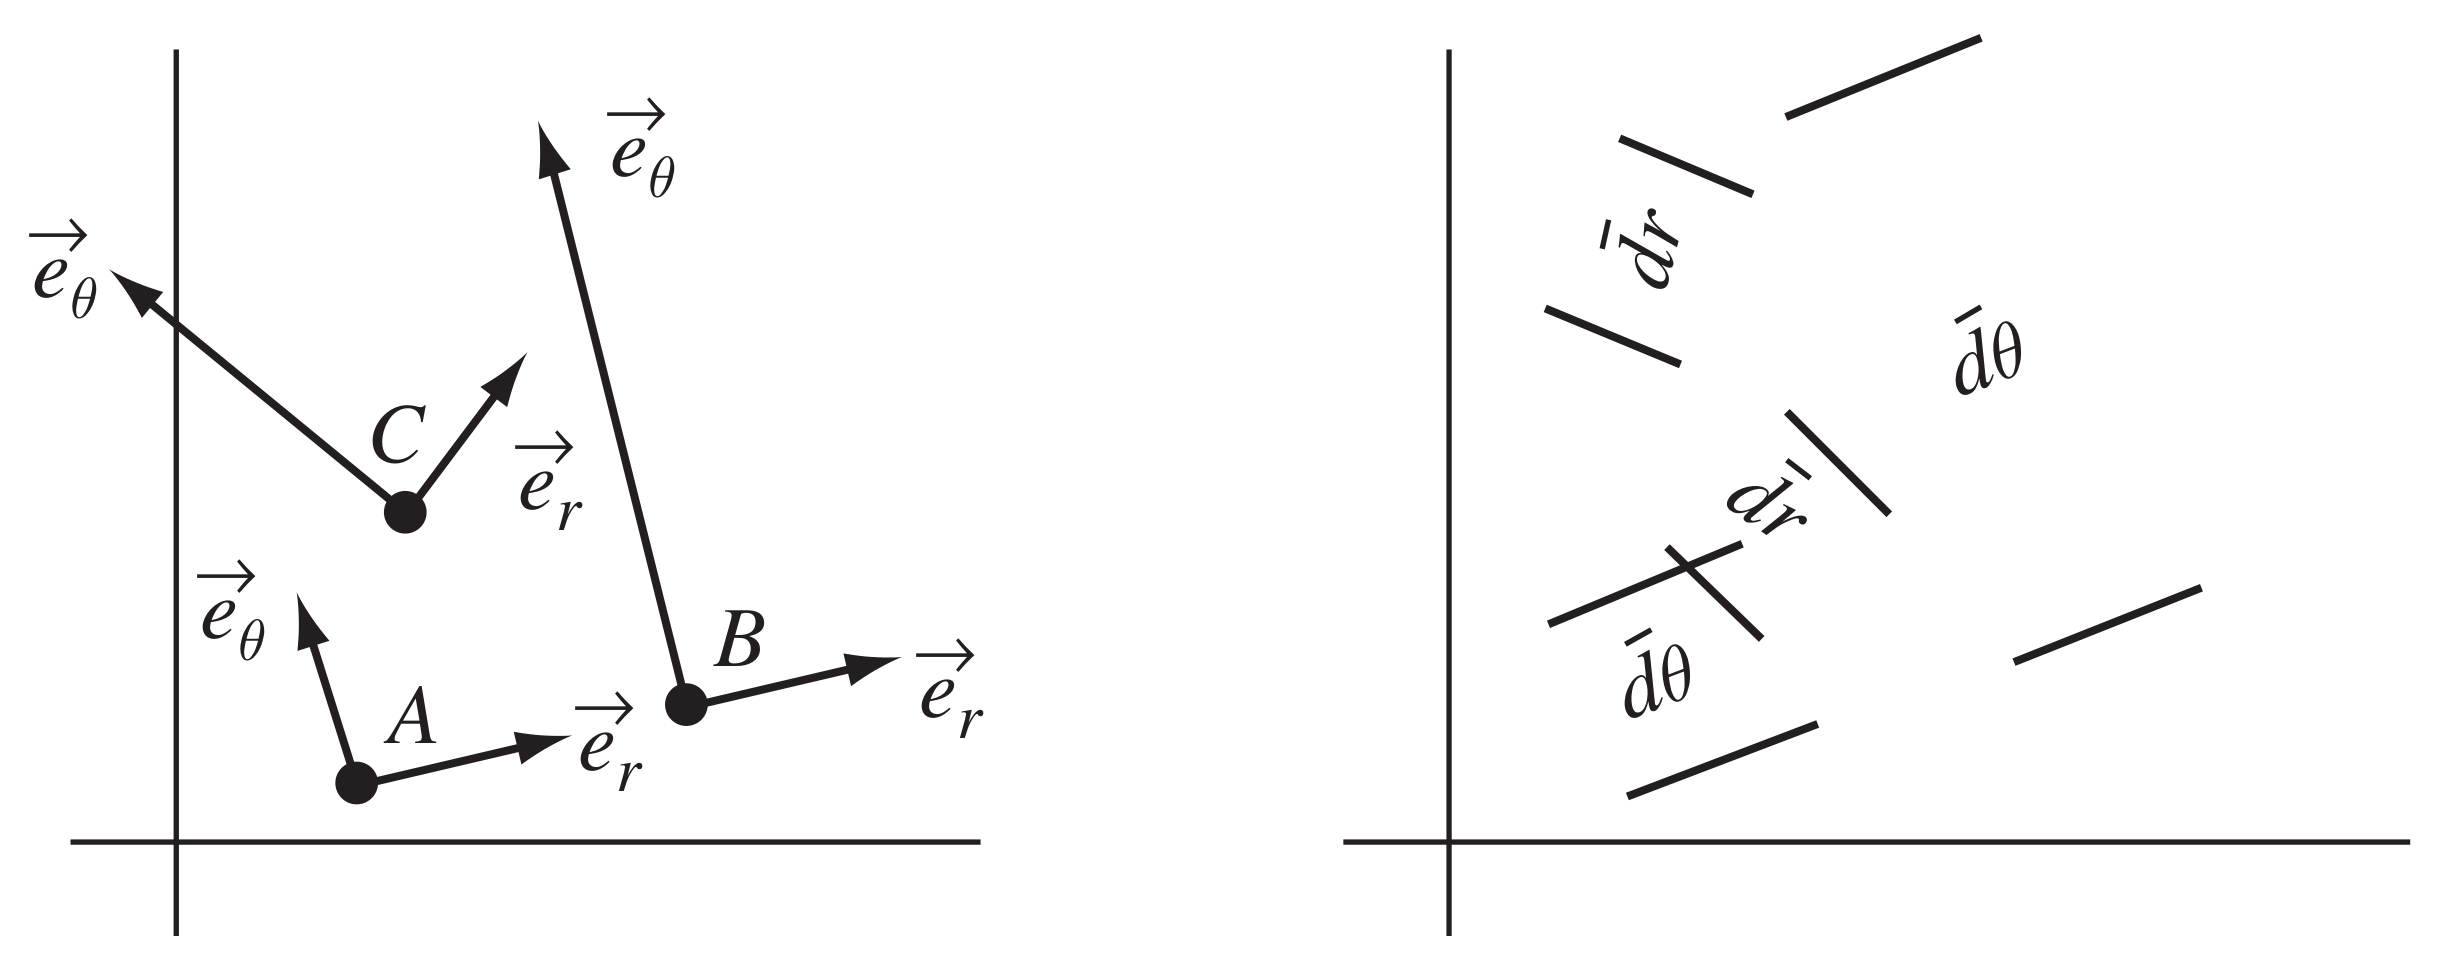
\includegraphics[width=0.7\textwidth]{fig5.5.png}
    \figcaption{极坐标系的向量基与1形式基图示}
    \label{fig5.5}
}

上面体现了一个非常重要的事实:各点的基互不相同。例如,图\ref{fig5.5}中$A$点与$C$点的向量基不平行。这是由于基向量指向坐标增加的方向,而这个方向随着点的改变而改变。此外,基的长度也不是恒定不变的。例如,根据\eqref{equ5.23}式可得

\begin{subequations}
\begin{alignat}{2}
    |\Ve_\theta|^2 &= \Ve_\theta \cdot \Ve_\theta = r^2 \sin^2 \theta + r^2 \cos^2 \theta = r^2,&& \label{equ5.28a} \\
    |\Ve_r| &= 1, \quad |\trd r| = 1, \quad |\trd \theta| = r^{-1}. &&\label{equ5.28b}
\end{alignat}
\end{subequations}
距离原点越远,$\Ve_\theta$的模长越大。因为$\Ve_\theta$在$(r, \theta)$系的分量为$(0, 1)$,意味着它表示$\theta$分量的1单位的位移,即1弧度。在半径更大的地方,移动1弧度的长度更大。因此极坐标基并非\textit{单位}基。其它基的模长容易求出。可以发现,$| \trd \theta|$在$r = 0$附近更大(更紧密),因为一个给定的向量在原点附近覆盖的$\theta$范围更大。

\subsection*{度规张量}
上面的点乘结果都是根据直角坐标系$x, y$中已知的度规来计算的:
\[
    \vec{e}_x \cdot \vec{e}_x = \vec{e}_y \cdot \vec{e}_y = 1, \quad \vec{e}_x \cdot \vec{e}_y = 0;
\]
或者用张量记号写为
\begin{equation}
    \mathbf{g} (\vec{e}_\alpha, \vec{e}_\beta) = \delta_{\alpha \beta} \quad \text{在直角坐标系中。}
\label{equ5.29}
\end{equation}
$\mathbf{g}$在极坐标系的分量是什么?根据分量的定义:
\begin{equation}
    g_{\alpha' \beta'} = \mathbf{g} (\vec{e}_{\alpha'}, \vec{e}_{\beta'}) = \vec{e}_{\alpha'} \cdot \vec{e}_{\beta'},
\label{equ5.30}
\end{equation}
或者根据\eqref{equ5.28}、\eqref{equ5.22}和\eqref{equ5.23}式可得
\begin{equation}
    g_{rr} = 1, \quad g_{\theta \theta} = r^2, \quad  g_{r \theta} = 0. \label{equ5.31}
\end{equation}
由此可得$\mathbf{g}$在极坐标系的分量为
\begin{equation}
    (g_{\alpha \beta})_{\text{polar}} = 
        \begin{pmatrix}
            1 & 0 \\
            0 & r^2
        \end{pmatrix},
\label{equ5.32}
\end{equation}
线元(line element)可以方便地同时表示$\mathbf{g}$的分量以及坐标,线元即为任意“无穷小”位移$\rd \vec{\ell}$的模:
\begin{shaded}
\begin{align}
    \rd \vec{\ell} \cdot \rd \vec{\ell} &= \rd s^2 = |\rd r \vec{e}_r + \rd \theta \vec{e}_\theta |^2 \notag \\
    &= \rd r^2 + r^2 \rd \theta^2. \label{equ5.33}
\end{align}
\end{shaded}
\textit{不要}将这里的$\rd r, \rd \theta$与1形式基$\trd r, \trd \theta$混淆,前者是$\rd \vec{\ell}$在极坐标系的分量,“$\rd$”就是“无穷小$\Delta$”的意思。 

另外有一种导出\eqref{equ5.33}式的方法值得一提。回顾\eqref{equ3.26}式,它表明任何$\binom{0}{2}$张量可以表示为$\binom{0}{2}$张量基$\trd x^\alpha \otimes \trd x^\beta$的线性组合:
\[
    \mathbf{g} = g_{\alpha \beta} \trd x^\alpha \otimes \trd x^\beta = \trd r \otimes \trd r + r^2 \trd \theta \otimes \trd \theta.
\]
尽管上式看起来像\eqref{equ5.33}式,但它们不一样:上式各项是算符,作用于向量$\rd \vec{\ell}$(其分量为$\rd r, \rd \theta$)之后得到\eqref{equ5.33}式。由于相应学科的符号混乱,导致上面两个式子非常不幸地十分相像。大多数教材与论文仍采用“旧式的”表达式——方程\eqref{equ5.33}来表示度规分量,本书遵从这一习惯。

度规分量矩阵存在逆矩阵:
\begin{equation}
    {\begin{pmatrix}
        1 & 0 \\
        0 & r^2
    \end{pmatrix} }^{-1} = 
    \begin{pmatrix}
        1 & 0 \\
        0 & r^{-2}
    \end{pmatrix}.
\label{equ5.34}
\end{equation}
由此可得$g^{rr} = 1, g^{r\theta} = 0, g^{\theta \theta} = 1/r^2$。这可以建立1形式与向量之间的映射。例如,向量场$\phi$的梯度场为$\trd \phi$,则这个1形式相应的向量$\rd \phi$具有分量
\begin{equation}
    (\vec{\rd} \phi)^\alpha = g^{\alpha \beta} \phi_{, \beta}
\label{equ5.35}
\end{equation}
或者写为
\begin{subequations}
\begin{alignat}{2}
    (\vec{\rd} \phi)^r &= g^{r \beta} \phi_{, \beta} = g^{rr} \phi_{, r} + g^{r \theta} \phi_{, \theta} \notag &&   \\
    &= \frac{\partial \phi}{\partial r}. &&\label{equ5.36a} \\
    (\vec{\rd} \phi)^\theta &= g^{\theta r} \phi_{, r} + g^{\theta \theta} \phi_{, \theta} && \notag \\
    &= \frac{1}{r^2} \frac{\partial \phi}{\partial \theta}. && \label{equ5.36b}
\end{alignat}
\end{subequations}
可见,1形式的分量是$(\phi_{, r}, \phi_{, \theta})$,而相应向量的分量是$(\phi_{, r}, \phi_{, \theta} / r^2)$。就算是在欧几里得空间,向量与相应的1形式的分量一般也不相同。直角坐标系是它们在其中唯一相等的坐标系。



\section{极坐标系的张量微积分}
\label{sec5.3}


\chapter{弯曲流形}
\label{chap6}

\section{微分流形,张量}
\label{sec6.1}

\subsection*{流形}

\subsection*{微分结构}
我们只考虑“微分流形”(differentiable manifolds),它们是连续且可微的空间。粗略地说,微分流形的每一点的邻域都可定义从该邻域到欧几里得空间的光滑映射,该映射保证标量函数的导数在那一点不变。球面是处处可微的,而锥面除了顶点以外处处可微。物理学用到的流形基本上都是几乎处处可微的,GR的弯曲流形就是如此。

可微性的条件直接意味着可以定义1形式与向量。也就是说,在流形上的某个坐标系中,集合$\{ \phi_{, \alpha} \}$的元素是1形式$\trd \phi$的分量;而集合$\{ a \phi_{, \alpha} + b \psi_{, \alpha} \}$(其中$a, b$是函数)也是1形式场。类似的,任何曲线(带有参数,例如$\lambda$)具有切向量$\vec{V}$,它定义为将1形式$\trd \phi$变成“标量场沿该曲线的导数$\rd \phi / \rd \lambda$”的线性函数:
\begin{equation}
    \langle \trd \phi, \vec{V} \rangle = \vec{V} (\trd \phi) = \nabla_{\vec{V}} \phi = \frac{\rd \phi}{\rd \lambda}.
\label{equ6.1}
\end{equation}
向量的线性组合也是向量。利用上面定义的向量和1形式,可以定义各种$\binom{M}{N}$型张量,就像SR里定义的那样。由于目前尚未钦点任何$\binom{0}{2}$张量为度规,因此向量与1形式之间还没有对应关系。不过其它内容与之前讨论的SR情形、极坐标系相同。这些内容都来自于微分,因此所有张量的集合称为流形的“微分结构 (differential structure)”的一部分。我们不会经常使用这个术语。


\subsection*{回顾}

\section{Riemannian流形}
\label{sec6.2}
目前为止尚未在流形中引入度规。在一些问题的流形中,度规是不必要或不常用的。但是对GR而言,度规绝对是最基本的,因为就像SR那样,度规描述了钟的走时与两点的距离。一个微分流形配上一个被选召为度规的、对称的$\binom{0}{2}$张量场$\bm{g}$,称为Riemannian流形(黎曼流形)。\textit{严格来说,只有当度规是正定的——即$\forall\, \vec{V} \neq 0, \bm{g} (\vec{V}, \vec{V}) > 0$——才叫做Riemannian流形;SR与GR那样的不定度规情况叫做pseudo-Riemannian(伪黎曼流形)。不过作为一本物理书我们并不区分统统称为Riemannian流形。} 选出一个度规意味着在流形上“添加”某种结构,理解这一点很关键,之后会看到这个度规完全定义了流形的曲率。因此,选定一个度规$\bm{g}$之后,流形具有了一种曲率(例如,球面),而选择另一个度规$\bm{g}'$流形具有另一种曲率(例如,旋转椭球面)。“原始的”微分流形自身是一团无定形的点的集合,并且局域地相似于欧几里得空间中的点的排布,其中的距离与形状并未指定。给定了度规$\bm{g}$就赋予了流形以特定形状,后面就会看到。从现在开始,我们讨论的对象是Riemannian流形,其上的每一点都定义了度规$\bm{g}$。

\textit{为了内容完整,我们指出,可以不利用度规来定义流形曲率的概念(称为“仿射 (affine)”流形)。有些文献用采用这种方法,但是度规在GR中的地位是基本的,因此我们利用度规定义流形曲率。}


\subsection*{度规,局域平直性}
自然,度规提供了每一点的向量与1形式之间的映射。因此,给定向量场$\vec{V} (\mathcal{P})$(这个符号意味着$\vec{V}$取决于位置$\mathcal{P}$,$\mathcal{P}$是流形中的任一点),它唯一对应于1形式场$\tilde{V} (\mathcal{P}) = \bm{g} (\vec{V} (\mathcal{P}), \ )$。这个映射必须是可逆的\sout{画外音:看不出来……},因此$\tilde{V} (\mathcal{P})$也对应唯一的$\vec{V} (\mathcal{P})$。$\bm{g}$的分量记作$g_{\alpha \beta}$;分量矩阵的逆矩阵记作$g^{\alpha \beta}$。度规可以升降指标,就像SR中的那样:
\[
    V_\alpha = g_{\alpha \beta} V^\beta.
\]
一般的$\{ g_{\alpha \beta} \}$是坐标的复杂函数,因此在一般的坐标系中,向量与1形式分量,例如$V^0$与$V_0$,一般没有简单的关系。

要研究一般的弯曲流形就要在一般的坐标系中考虑问题。SR只在Lorentz系(惯性系)中讨论(因为简单),但是引力使得全局惯性系不存在,因此我们得考虑所有的(一般性的)坐标系,以及所有的(一般性的)非奇异坐标变换。\textit{非奇异性在\ref{sec5.2}节介绍过,它意味着变换矩阵$\Lambda\indices{^{\alpha'}_\beta} \equiv \partial x^{\alpha'} / \partial x^\beta$可逆。} 根据定义,度规分量矩阵$(g_{\alpha \beta})$是对称的,线性代数的一条重要定理(见第\ref{chap6}章习题3)告诉我们,对于任意对称矩阵$(g_{\alpha' \beta'})$,总可以找到变换矩阵将$(g_{\alpha' \beta'})$化为对角元是$+1, -1$或0的对角矩阵,且$+1$的数量等于矩阵$(g_{\alpha' \beta'})$的正特征值的个数、$-1$的数量等于负特征值个数。故而,如果一开始选择$\bm{g}$的分量矩阵具有3个正特征值、1个负特征值,则总可以找到变换矩阵$\Lambda\indices{^{\alpha'}_\beta}$使得度规分量变换为:
\begin{equation}
    (g_{\alpha' \beta'}) = 
    \begin{pmatrix}
        -1 & 0 & 0 & 0 \\
        0 & 1 & 0 & 0 \\
        0 & 0 & 1 & 0 \\
        0 & 0 & 0 & 1
    \end{pmatrix}
    \equiv (\eta_{\alpha \beta}).
\label{equ6.2}
\end{equation}
今后,$\eta_{\alpha \beta}$ \textit{专指}上式中的矩阵,也就是SR的度规。

有两点重要内容必须指出。第一,只有$(g_{\alpha \beta})$选为3个正特征值、1个负特征值的时候,\eqref{equ6.2}式才可能。\eqref{equ6.2}式矩阵的对角元素之和称为度规的\textit{号差 (signature)},SR与GR的度规号差都是$+2$。因此,之前我们论述过,在任意事件处总可以构造一个\textit{局域}惯性系,方程\eqref{equ6.2}是这个物理命题的数学表述,亦即,该点的度规总可以变换为$\eta_{\alpha \beta}$。反过来,这意味着一个描述有引力时空的度规的号差必须是$+2$。

第二,\eqref{equ6.2}式对应的变换矩阵$\Lambda\indices{^{\alpha'}_\beta}$也许\textit{并非}坐标变换。也就是说,集合$\{ \tilde{\omega}^{\alpha'} = \Lambda\indices{^{\alpha'}_\beta} \trd x^\beta \}$也许不是坐标基。根据前面对非坐标基的讨论,$\Lambda\indices{^{\alpha'}_\beta}$只有当\eqref{equ5.95}式成立时才是坐标变换:
\[
    \frac{\partial \Lambda\indices{^{\alpha'}_\beta}}{\partial x^\gamma} = \frac{\partial \Lambda\indices{^{\alpha'}_\gamma}}{\partial x^\beta}.
\]

这在一般的引力场中不能成立,否则就意味着存在\eqref{equ6.2}式处处成立的坐标系——全局惯性系了。不过,既然可以使\eqref{equ6.2}式在$\mathcal{P}$点成立,那么也可以找到坐标系使得\eqref{equ6.2}式在$\mathcal{P}$点的邻域“近似”成立。这体现在如下的定理中,该定理的证明(相当长)见本节最后。对于流形上的任一点$\mathcal{P}$,可以找到原点为$\mathcal{P}$点的坐标系$\{ x^\alpha \}$,在该坐标系中:
\begin{equation}
    g_{\alpha \beta} (x^\mu ) = \eta_{\alpha \beta} + 0 [(x^\mu)^2].
\label{equ6.3}
\end{equation}
这意味着,$\mathcal{P}$点附近的度规近似是SR的度规,相差坐标的二阶量。今后称这种坐标系为“\textbf{局域Lorentz系}”或“\textbf{局域惯性系} (local inertial frames, \textbf{LIF})”。方程\eqref{equ6.3}可以表示为更精确的形式:
\begin{shaded}
\begin{align}
    g_{\alpha \beta} (\mathcal{P}) &= \eta_{\alpha \beta} \quad \forall\, \alpha, \beta; \label{equ6.4} \\
    \frac{\partial}{\partial x^\gamma} g_{\alpha \beta} (\mathcal{P}) &= 0 \quad \forall\, \alpha, \beta, \gamma; \label{equ6.5}
\end{align}
\end{shaded}
但是在一般情况下
\begin{shaded}
\begin{equation*}
    \frac{\partial^2}{\partial x^\gamma \partial x^\mu} g_{\alpha \beta} (\mathcal{P}) \neq 0
\end{equation*}
\end{shaded}
在弯曲流形中,上式至少对某些$\alpha, \beta, \gamma, \mu$成立。

局域惯性系的存在性等价于弯曲空间中的任一点存在“相切”的平坦空间。平直时空中,自由粒子的世界线是直线;方程\eqref{equ6.5}中弯曲时空度规的一阶导数项为零意味着,弯曲时空中的自由粒子沿着在局域惯性系中的“局域直”的线运动。由于物理学方程在平直时空中最简单,而按照\ref{sec6.1}节总结的规律,只要在局域惯性系写出张量等式的方程,则该方程在任意坐标系都有效,因此局域惯性系十分有用。别忘了定理的证明在本节最后,尽管比较长,但是它值得研究。

\subsection*{长度与体积}
度规定义了曲线的长度。将曲线上的无穷小位移向量记作$\rd \vec{x}$,则$\rd \vec{x}$长度的平方$\rd s^2 = g_{\alpha \beta} \rd x^\alpha \rd x^\beta$(回顾一下,前面称之为度规的\textit{线元})。对它的绝对值开平方就是长度:$\rd \ell \equiv |  g_{\alpha \beta} \rd x^\alpha \rd x^\beta |^{1/2}$,再进行积分:
\begin{align}
    \ell &= \int_{\text{沿曲线}} | g_{\alpha \beta} \rd x^\alpha \rd x^\beta | ^{1/2} \label{equ6.6} \\
    &= \int_{\lambda_0}^{\lambda_1} \left| g_{\alpha \beta} \frac{\rd x^\alpha}{\rd \lambda} \frac{\rd x^\beta}{\rd \lambda} \right|^{1/2} \, \rd \lambda, \label{equ6.7}
\end{align}
其中$\lambda$是曲线的参数(端点处的参数值为$\lambda_0, \lambda_1$)。由于曲线的切向量$\vec{V}$的分量为$V^\alpha = \rd x^\alpha / \rd \lambda$,上式可写为:
\begin{shaded}
\begin{equation}
    \ell = \int_{\lambda_0}^{\lambda_1} | \vec{V} \cdot \vec{V} |^{1/2} \, \rd \lambda,
\label{equ6.8}
\end{equation}
\end{shaded}
这就是任意曲线的长度。

在对时空区域进行积分时,计算体积十分重要。这里的“体积”是指四维体积元,它出现于\ref{sec4.4}节Gauss定律的积分中。局域惯性系的无穷小四维体元的四维体积为$\rd x^0\, \rd x^1\, \rd x^2\, \rd x^3$,其中$\{ x^\alpha \}$是原点在指定点的局域惯性系,满足方程\eqref{equ6.3}。在\textit{任意}坐标系$\{ x^{\alpha'}\}$中,根据多变量微积分的知识可得:
\begin{equation}
    \rd x^0\, \rd x^1\, \rd x^2\, \rd x^3 = \frac{\partial (x^0, x^1, x^2, x^3)}{\partial (x^{0'}, x^{1'}, x^{2'}, x^{3'}) } \rd x^{0'}\, \rd x^{1'}\, \rd x^{2'}\, \rd x^{3'},
\label{equ6.9}
\end{equation}
其中$\partial (\ ) / \partial (\ )$是从$\{ x^{\alpha'} \}$到$\{ x^\alpha \}$的变换的Jacobian(雅可比行列式),在\ref{sec5.2}节定义过:
\begin{align}
    \frac{\partial (x^0, x^1, x^2, x^3)}{\partial (x^{0'}, x^{1'}, x^{2'}, x^{3'}) } &= \det \begin{pmatrix}
        \partial x^0 / \partial x^{0'} & \partial x^0 / \partial x^{1'} & \dots \\
        \partial x^1 / \partial x^{0'} & \ & \  \\
        \vdots &&
    \end{pmatrix} \notag \\
    &= \det (\Lambda\indices{^\alpha_{\beta'}}). \label{equ6.10}
\end{align}
计算Jacobian的过程相当繁琐,不过利用度规可以简化计算过程。度规分量变换的矩阵形式为
\begin{equation}
    (g) = (\Lambda) (\eta) (\Lambda)^T,
\label{equ6.11}
\end{equation}
其中$(g)$表示矩阵$g_{\alpha \beta}$,$(\eta)$表示$\eta_{\alpha \beta}$,等等。符号$T$表示矩阵转置。上式取行列式:
\begin{equation}
    \det (g) = \det (\Lambda) \, \det (\eta) \, \det (\Lambda^T).
\label{equ6.12}
\end{equation}
转置矩阵的行列式与原矩阵相等:
\begin{equation}
    \det (\Lambda) = \det (\Lambda^T),
\label{equ6.13}
\end{equation}
而根据\eqref{equ6.2}可得
\begin{equation}
    \det (\eta) = -1.
\label{equ6.14}
\end{equation}
综上,
\begin{equation}
    \det (g) = - [\det (\Lambda)]^2.
\label{equ6.15}
\end{equation}
引入记号
\begin{equation}
    g := \det( g_{\alpha' \beta'}),
\label{equ6.16}
\end{equation}
这样方程\eqref{equ6.15}可以写为
\begin{equation}
    \det (\Lambda\indices{^\alpha_{\beta'}}) = (-g)^{1/2}.
\label{equ6.17}
\end{equation}
从而,根据\eqref{equ6.9}式可得:
\begin{shaded}
\begin{align}
    \rd x^0\, \rd x^1\, \rd x^2\, \rd x^3 &= \big[ -\det (g_{\alpha' \beta'}) \big]^{1/2} \, \rd x^{0'}\, \rd x^{1'}\, \rd x^{2'}\, \rd x^{3'} \notag \\
    &= (-g)^{1/2} \, \rd x^{0'}\, \rd x^{1'}\, \rd x^{2'}\, \rd x^{3'}. \label{equ6.18}
\end{align}
\end{shaded}
这个结果非常有用。这个式子的推导思路也很重要,因为这是第一个利用局域惯性系将平直时空的结果推广到弯曲时空的例子,之后会经常利用这种思路。本例从局域惯性系的体元$\rd x^0\, \rd x^1\, \rd x^2\, \rd x^3 = \rd^4 x$出发,由于给定点附近的时空邻域和Minkowski空间相同,因此这个体元就是可以由时钟与尺子测量的物理量。接着我们导出了在任意坐标系$\{ x^{\mu'} \}$的体元表达式\eqref{equ6.18},$(-g)^{1/2} \rd^4 x'$,这就是弯曲时空中任意坐标系的任一点的物理体积元,我们称之为\textit{固有体元 (proper volume element)}。

度规出现在固有体元里,这是在意料之中的,因为度规测量长度。任意坐标系的$\rd^4 x$乘以$(-g)^{1/2}$就得到的真实的,或者说\textit{固有的(proper)}体元。

这里应该举个三次元欧几里得空间的例子,由于该空间的度规是正定的(\eqref{equ6.14}的对应结果是$+1$),因此固有体元应该乘以$(g)^{1/2}$。球坐标系的线元$\rd \ell^2 = \rd r^2 + r^2 \rd \theta^2 + r^2 \sin^2 \theta \rd \phi^2$,因此度规是
\begin{equation}
    (g_{ij}) = 
    \begin{pmatrix}
        1 & 0 & 0 \\
        0 & r^2 & 0 \\
        0 & 0 & r^2 \sin^2 \theta
    \end{pmatrix}.
\label{equ6.19}
\end{equation}
度规行列式等于$r^4 \sin^2 \theta$,所以固有体元$(g)^{1/2} \, \rd^3 x'$等于
\begin{equation}
    r^2 \sin \theta \rd r \rd \theta \rd \phi,
\label{equ6.20}
\end{equation}
这就是人们熟悉的极坐标系的体积元。

\subsection*{局域平直性定理的证明}
记$\{ x^\alpha \}$是任意坐标系,$\{ x^{\alpha'}\}$是局域惯性系:它在所考虑的$\mathcal{P}$点附近简化为惯性系(四维时空流形中的点就是一个事件)。这两个坐标系之间的坐标变换为:
\begin{align}
    x^\alpha &= x^\alpha (x^{\mu'}), \label{equ6.21} \\
    \Lambda\indices{^\alpha_{\mu'}} &= \partial x^\alpha / \partial x^{\mu'}. \label{equ6.22}
\end{align}
将$\Lambda\indices{^\alpha_{\mu'}}$在$\mathcal{P}$点(该点的坐标是$x_0^{\mu'}$)附近作Taylor展开,其中$\vec{x}$是$\mathcal{P}$点附近的一点:
\begin{align}
    \Lambda\indices{^\alpha_{\mu'}} (\vec{x}) =& \Lambda\indices{^\alpha_{\mu'}} (\mathcal{P}) + (x^{\gamma'} - x_0^{\gamma'}) \frac{\partial \Lambda\indices{^\alpha_{\mu'}}}{\partial x^{\gamma'}} (\mathcal{P}) \notag \\
    &+ \frac{1}{2} (x^{\gamma'} - x_0^{\gamma'}) (x^{\lambda'} - x_0^{\lambda'}) \frac{ \partial^2 \Lambda\indices{^\alpha_{\mu'}} }{ \partial x^{\lambda'} \partial x^{\gamma'} } (\mathcal{P}) + \dots , \notag \\
    =& \Lambda\indices{^\alpha_{\mu'}}\Bigg|_{\mathcal{P}} + (x^{\gamma'} - x_0^{\gamma'} ) \frac{ \partial^2 x^\alpha }{ \partial x^{\gamma'} \partial x^{\mu'} } \Bigg|_{\mathcal{P}} \notag \\
    &+ \frac{1}{2} (x^{\gamma'} - x_0^{\gamma'})(x^{\lambda'} - x_0^{\lambda'}) \frac{ \partial^3 x^\alpha }{ \partial x^{\lambda'} \partial x^{\gamma'} \partial x^{\mu'} } \Bigg|_{\mathcal{P}} + \dots. \label{equ6.23}
\end{align}


\section{协变微分}
\label{sec6.3}

\section{平行移动,测地线,曲率}
\label{sec6.4}

\section{曲率张量}
\label{sec6.5}

\section{Bianchi恒等式:Ricci张量与Einstein张量}
\label{sec6.6}

\section{Curvature in perspective}
\label{sec6.7}

\section{扩展阅读}
\label{sec6.8}

\section{习题}
\label{sec6.9}


\chapter{弯曲时空中的物理学}
\label{chap7}

\section{微分几何与引力理论的对应}
\label{sec7.1}
将物理理论用数学形式表达,本质上是将数学概念与可观测物理量联系起来。因此我们首先要把之前建立的几何概念与现实世界的引力进行对应,这之前已经多少讨论过了,例如我们假设时空是个微分流形,并且已经证明了在非均匀引力场下不存在全局惯性系,在这些论述之后是如下的两条对应:

\begin{shaded}
\begin{enumerate}
    \item[(\uppercase\expandafter{\romannumeral1})] 时空(所有事件的集合)是带有度规的四维流形。
    \item[(\uppercase\expandafter{\romannumeral2})] 度规可以由杆与钟测量。用杆测量的相邻两事件点(它们的时间相同)的空间间距是$|\rd \vec{x} \cdot \rd \vec{x}|^{1/2}$,用钟测量的时间相近的两事件点(它们的空间位置相同)的时间间隔是$|-\rd \vec{x} \cdot \rd \vec{x}|^{1/2}$。
\end{enumerate}
\end{shaded}
一般不存在一个坐标系使得$\rd \vec{x} \cdot \rd \vec{x} = -(\rd x^0)^2 + (\rd x^1)^2 + (\rd x^2)^2 + (\rd x^3)^2$处处成立。另一方面,我们论证了这种坐标系在\textbf{局域上}是存在的。这显然对应着弯曲流形,在其中任一点附近都存在坐标系局域的与Minkowski时空相似(例如向量的点乘形式)。

据此可以进行如下的对应条件:
\begin{shaded}
\begin{enumerate}
    \item[(\uppercase\expandafter{\romannumeral3})] 在任一事件点附近,存在合适的坐标系使得时空的度规为Lorentz形式$\eta_{\alpha \beta}$。
\end{enumerate}
\end{shaded}
在钦定了这种表示时空的方式之后,还需要完成两点才能得到完整的理论。第一,必须说明物理对象(粒子、电场、流体等等)在弯曲时空中如何表现;第二,必须说明时空中的物体是怎样产生或着决定曲率的。

作为物理理论的例子,我们先来考虑牛顿引力理论。牛顿理论的时空是三维欧几里得空间加上一维时间轴(数学上的记号是$R^3 \times R$)。不存在整体时空流形上的度规,空间距离来自欧几里得空间自带的普通度规、时间由绝对的“宇宙钟”测量。速度不同的观测者地位相同:这是伽利略力学里的相对性。因此不存在绝对静止的参照物,并且不同观者对于两个不同时的事件是否发生于同一地点的结论可能不同。但是所有观者的同时性——即两个事件是否在同一时间(时间轴的同一切片)发生——是绝对的,所以两个事件的“时间间隔”意味着包含两个事件的欧几里得切面之间经过的时间。它与事件的空间位置无关,因此牛顿引力理论中的时间是绝对的:所有观者,无论位置或运动状态如何,观测到的两事件的时间间隔都相同。类似地,两事件的“空间间隔”的含义是两事件在欧几里得空间的距离。如果两个时间是同时的(发生于时间轴的同一欧几里得切片),则利用那个切片的空间度规即可计算空间间隔,所有观测者的结果相同。如果两个事件发生的时间不同,则每个观者取他所观测到的事件的切片并计算空间间隔,不同观者观测到的事件的坐标不同,但距离都相同。

然而,在牛顿理论中无法将时间与距离观测结合起来: there was no invariant measure of the length of a general curve that changed position and time as it went along. 没有将时间与空间距离相互转换的不变量,也就无法进行结合。爱因斯坦为相对论引入了不变量——光速,它将空间与时间的观测量统一起来。爱因斯坦四维时空的结构实际上比牛顿的绝对时空更加简单!

在绝对时空的模型下,牛顿给出了描述物体受引力影响的定律:$\bm{F} = -m \bm{a}$,其中$\bm{F} = -m \nabla \phi$是物体在给定引力场$\phi$当中所受的引力。牛顿也给出了物体是如何产生引力场$\phi$的:$\nabla^2 \phi = 4\pi G \rho$。时空的相对论描述必须给出这两个定律的对应版本,第二个式子的对应在下一章讨论,本章研究一个给定的度规是如何影响时空中的物体的。

之前讨论过粒子运动的简单情况。我们知道粒子在引力场中的“加速度”与粒子质量无关,因此在附近的自由下落参考系中粒子加速度为零,这就对应于局域惯性系。因为自由下落粒子在该系的加速度为零,因此粒子(至少是局域地)沿直线运动。局域惯性系的直线正是弯曲流形的测地线的\textbf{定义}。这样我们得到了关于粒子受度规影响的第一条假设:

\begin{shaded}
\begin{enumerate}
    \item[(\uppercase\expandafter{\romannumeral4})] \textbf{弱等效原理 (Weak Equivalence Principle, WEP)}:自由下落粒子沿时空的类时测地线运动。\footnote{WEP更普遍的定义没有涉及弯曲时空,而只是说粒子在引力场的下落速度相同(不依赖于粒子质量与位置)。但是爱因斯坦等效原理(假设$\uppercase\expandafter{\romannumeral4}'$意味着引力可以由时空曲率表示,因此我们以弯曲时空作为讨论的出发点。}
\end{enumerate}
\end{shaded}
“自由下落”意味着粒子不受其它力影响,例如电场力等等。其它所有的力与引力的区别在于,\textbf{存在着}不受其它力作用的粒子。因此弱等效原理(假设\uppercase\expandafter{\romannumeral4})是很强的陈述,它可以被实验检验。WEP饱经、并且一直在经受高精度的检验,其中典型的实验例如比较由不同材料组成的物体的下落速度;当前的对加速度差别的实验限制已经到了$10^{13}$量级(Will 2006)。因此WEP是被实验验证的精度最高的物理定律之一。人们计划利用卫星搭载的实验来将精度提高到$10^{-18}$量级。

不过,WEP只针对粒子,其它对象(例如流体)是如何受非平直度规影响的?为此需要将\uppercase\expandafter{\romannumeral4}进行推广:

\begin{shaded}
\begin{enumerate}
    \item[(\uppercase\expandafter{\romannumeral4})$'$] \textbf{爱因斯坦等效原理 (Einstein Equivalence Principle, EEP)}:任何不涉及引力的、局域的物理实验,在(弯曲时空中的)自由下落惯性系的结果与在平直时空(狭义相对论有效)中的结果相同。
\end{enumerate}
\end{shaded}
其中,“局域”的含义是实验不涉及场,例如电场,场延伸到一大片时空区域,超出了局域惯性系的有效范围。所有的\textbf{局域}物理结果在自由下落惯性系的结果,与狭义相对论的结果相同。引力\textbf{局域上}没有引入任何新内容,所有引力的效应要在时空中延伸一定的区域才能感受到,这也被实验严格检验过了(Will 2006)。

(未完成)

This may seem strange to someone used to blaming gravity for making it hard to climb
stairs or mountains, or even to get out of bed! But these local effects of gravity are, in
Einstein’s point of view, really the effects of our being pushed around by the Earth and
objects on it. Our ‘weight’ is caused by the solid Earth exerting forces on us that prevent us
from falling freely on a geodesic (weightlessly, through the floor). This is a very reasonable
point of view. Consider astronauts orbiting the Earth. At an altitude of some 300 km, they
are hardly any further from the center of the Earth than we are, so the strength of the
Newtonian gravitational force on them is almost the same as on us. But they are weightless,
as long as their orbit prevents them encountering the solid Earth. Once we acknowledge
that spacetime has natural curves, the geodesics, and that when we fall on them we are in
freefallandfeelnogravity,thenwecandisposeoftheNewtonianconceptofagravitational
force altogether. We are only following the natural spacetime curve.


The true measure of gravity on the Earth are its tides. These are nonlocal effects, because
they arise from the difference of the Moon’s Newtonian gravitational acceleration across
the Earth, or in other words from the geodesic deviation near the Earth. If the Earth were
permanently cloudy, an Earthling would not know about the Moon from its overall grav-
itational acceleration, since the Earth falls freely: we don’t feel the Moon locally. But
Earthlings could in principle discover the Moon even without seeing it, by observing and
understanding the tides. Tidal forces are the only measurable aspect of gravity.

爱因斯坦等效原理数学上的含义是(粗略地说),如果一条局域的物理定律在SR中写成了张量方程,则该定律在弯曲时空的局域惯性系中的数学形式也是如此。

这一原理经常被称作“逗号变分号规则”,因为如果定律的SR形式含有导数(逗号),则它在局域惯性系中也是如此。为了让方程在\textbf{任意}坐标系都有效,只需要在局域惯性系中把普通导数换成协变导数(分号),\footnote{当然,这样做的理由是Christoffel符号在局域惯性系的原点处等于零,前面用过很多次了。——译者} 这是一种超级简单地推广物理定律的方式。特别地,这一原理禁止了“曲率耦合”:例如热力学在弯曲时空的真正形式可能含有Riemann张量,而在SR中Riemann张量的相关内容会消失不见。假设(\uppercase\expandafter{\romannumeral4})$'$不允许Riemann张量有关的项出现在方程中。

下面举例说明怎样将((\uppercase\expandafter{\romannumeral4})$'$)转换为数学形式,以流体动力学(它是本课程的主要研究对象)为例。SR中的粒子数守恒定律表示为
\begin{equation}
    (n U^\alpha)_{, \alpha} = 0,
\label{equ7.1}
\end{equation}
其中$n$是瞬时共动参考系(MCRF)的粒子数密度,而$U^\alpha$是流体元的四速。在弯曲时空中的任意事件处,可以可以找到与该事件处的流体元瞬时共动的局域惯性系,并且按类似的方式定义$n$,同样,可以像SR那样定义四速$\vec{U}$是那个坐标系的时间基向量。于是,根据爱因斯坦等效原理,粒子数守恒律在局域惯性系的形式\textbf{正是}\eqref{equ7.1}式。由于Christoffel符号在给定事件点(该点是局域惯性系的原点)处等于零,\eqref{equ7.1}式等价于
\begin{equation}
    (n U^\alpha)_{; \alpha} = 0.
\label{equ7.2}
\end{equation}
这种张量方程的形式在\textbf{任何}坐标系都成立,从而利用上式就可以在任意坐标系中计算粒子数守恒,还要记住上式源于爱因斯坦等效原理。

这样,我们将粒子数守恒律推广到了弯曲时空。在之后需要的场合,我们总是利用这种方法推广物理定律。

上述内容仅仅是张量的游戏,还是蕴含着新的物理意义?弯曲时空中的粒子守恒律可能是\eqref{equ7.2}以外的形式吗?有可能。考虑如下形式:
\begin{equation}
    (n U^\alpha)_{; \alpha} = qR^2,
\label{equ7.3}
\end{equation}
其中$R$是Ricci标量,定义在\eqref{equ6.92}式,它是Riemann张量的两次缩并;$q$是常数。由于平直时空的Riemann张量为零,因此上式也会退化到SR形式\eqref{equ7.1}式。但是在弯曲时空中,上式预言的内容完全不同:曲率可以产生或湮灭粒子(与$q$的符号有关)。上两式都和SR的形式相符。爱因斯坦等效原理断言,应该把\eqref{equ7.1}式推广为尽量简单的形式,也就是\eqref{equ7.2}。当然,决定\eqref{equ7.2}和\eqref{equ7.3}式哪个正确要靠实验或者天文观测。本书采用绝大多数的观点——爱因斯坦等效原理是正确的。没有什么观测性证据反对它。

类似地,SR中的熵守恒定律是
\begin{equation}
    U^\alpha S_{, \alpha} = 0.
\label{equ7.4}
\end{equation}
因为标量$S$的协变导数不含Christoffel符号,所以上式在弯曲时空的形式\textbf{不变}。

最后,四动量守恒定律为
\begin{equation}
    T\indices{^{\mu \nu}_{, \nu}} = 0.
\label{equ7.5}
\end{equation}
推广到弯曲时空的形式为
\begin{equation}
    T\indices{^{\mu \nu}_{; \nu}} = 0.
\label{equ7.6}
\end{equation}
其中能动张量的定义与之前相似:
\begin{equation}
    T^{\mu \nu} = (\rho + p) U^\mu U^\nu + p g^{\mu \nu}.
\label{equ7.7}
\end{equation}
(注意,$g^{\mu \nu}$在局域惯性系等于平直时空度规$\eta^{\mu \nu}$.)

\section{轻微弯曲时空的物理学}
\label{sec7.2}


%!TEX root = ../CallenThermo.tex
%----------------------------------------------------------------------------------------
%	翻译:哪吒儿闹海
%   校对:lh1962
%----------------------------------------------------------------------------------------


\chapter{热力学系统的稳定性}
\label{chap8}
\section{热力学系统的内在稳定性}
\label{sec8.1}
热力学中基本的极值原理指出:$\text{d}S=0$以及$\text{d}^2S<0$。第一个式子表示系统的熵取极值,第二个表明这个极值是极大值. 第二个式子决定着系统的{\it 稳定性},然而之前我们还没有完整地考察过这个式子. 与此相似,在力学中,一个单摆的稳定位置是其势能最小的位置. 而所谓处在“不稳定平衡”的位置与此相反,它正好在势能最大的地方.

对稳定性的考量将催生一些热力学中有趣且重要的结论. 在本章中考察可使系统达到稳定的条件. 在第9章中我们会讨论不稳定性的结果——相变.

现在考虑两个完全相同的子系统,它们的基本方程都是$S=S(U,V,N)$,这两个子系统由完全不透的隔板分开. 假设$S$对$U$的依赖关系大致如图\ref{fig8.1}所示. 现在我们从第一个子系统中挪出$\Delta U$的能量到第二个系统中去,这时,总系统(由这两个子系统所组成)的熵就会由$2S(U,V,N)$变为$S(U+\Delta U,V,N)+S(U-\Delta U,V,N)$. 由图中可看出,总系统的熵竟然增大了\mpar{请回忆 Jensen 不等式,并批判性的看待作者的讨论。}. 显然,如果绝热限制被移除,那么能量就会自发地从一子系统流向另一个子系统,因之其中一个的能量会增多(温度也增加),另一个的能量减少. 这种情况甚至可以发生在一个子系统内,即能量从一个区域自发地转移到另一个区域,导致系统的均一性被破坏. 这种均一性的自发破缺就是相变的特征.

\begin{figure}
\centering
\includegraphics[width=\textwidth]{Pictures/fig8.1.png}
\figcaption{如图所示,对于下凹的基本关系,通过两个子系统的能量交换,平均熵增加了,这样的系统是不稳定的。}
\label{fig8.1}
\end{figure}

从图\ref{fig8.1}中我们可以看出,系统稳定的条件就是熵曲线{\it 上凹}.\footnote{R. B. Griffiths, \textit{J. Math. Phys.} \textbf{5}, 1215 (1964). L. Galgani and A. Scotti, \textit{Physica} \textbf{40}, (1968);\textbf{42},242(1969); \textit{Pure and Appl Chem.} \textbf{22}, 229(1970).}

\begin{equation}
\label{equ8.1}
S(U+\Delta U,V,N)+S(U-\Delta U,V,N)\leq 2S(U,V,N) \quad(\text{for all }\Delta)
\end{equation}

如果$\Delta U\to 0$,那么该条件就变为微分式
\begin{equation}
\label{equ8.2}
\left(\frac{\partial^2S}{\partial U^2}\right)_{V,N}\leq 0
\end{equation}
但是这个微分式没上凹条件\eqref{equ8.1}那么严格
,上凹条件需对所有的$\Delta U$成立,而非仅仅在$\Delta\to 0$时成立.

上面我们考虑的是能量的变化,如果我们考察体积的变化,结果是一样的
\begin{equation}
\label{equ8.3}
S(U,V+\Delta V,N)+S(U,V-\Delta V,N)\leq 2S(U,V,N)
\end{equation}
或写成微分形式
\begin{equation}
\label{equ8.4}
\left(\frac{\partial^2S}{\partial V^2}\right)_{U,N}\leq 0
\end{equation}

\begin{figure}
\centering
\includegraphics[width=.8\textwidth]{Pictures/fig8.2.png}
\figcaption{}
\label{fig8.2}
\end{figure}

在由统计力学计算所得和实验数据外推所得的基本方程中,有一些确实不满足上凹条件.这时如果非要得到一个稳定的基本方程的话,我们可以按照图\ref{fig8.2}所示的方法构造. 在真实的基本方程曲线上作切线,取那些处在曲线上方的切线,{\it 稳定的状态方程就是这些取出来的切线的上包络线}.

图\ref{fig8.2}中,BCDEF线是不稳定的,这一可用直线BHF来代替. 实际上,真实的状态方程中,只有CDE段不满足微分形式的稳定性条件(也就是说局部不满足上凹条件). 因此整个曲线就不满足“全局”性的上凹条件\eqref{equ8.1}.所以我们说该曲线中的BC和EF部分都是局域稳定但全局不稳定的.

直线(图\ref{fig8.2}中的BHF)对应着两个相的分离,即系统中的一部分处于B状态,而另一部分处于F状态,我们将在第9章中详细解释这个问题.

在$S-U-V$组成的三维空间中,全局稳定要求熵曲面处于它的所有切面之下. 也就是说
\begin{equation}
\label{equ8.5}
S(U+\Delta U,V+\Delta V,N)+S(U-\Delta U,V-\Delta V,N)\leq 2S(U,V,N)
\end{equation}
由该式可推得\eqref{equ8.2}、\eqref{equ8.4}和(参见问题8.1-1)
\begin{equation}
\label{equ8.6}
\frac{\partial^2S}{\partial U^2}\frac{\partial^2S}{\partial V^2}-\left(\frac{\partial^2S}{\partial U\partial V}\right) \ge 0
\end{equation}
我们待会儿会通过另一种方法得到这个等式:将一个类似\eqref{equ8.2}式的简单的曲率条件代入熵的Legendre变换.

再次强调,全局稳定要求熵曲面处于它的所有切面之下. 相较之下,局部稳定要求的条件就弱一些,它只要求$\left(\frac{\partial^2S}{\partial U^2}\right)_{V,N}$和$\left(\frac{\partial^2S}{\partial V^2}\right)_{U,N}$都是负的且$\frac{\partial^2S}{\partial U^2}\frac{\partial^2S}{\partial V^2}-\left(\frac{\partial^2S}{\partial U\partial V}\right)^2$是正的.
$\frac{\partial^2S}{\partial U^2}<0$保证了:体积为常数的平面与S-U-V曲面的交线曲率为负(线上每一处都是平衡点).同样,$\frac{\partial^2S}{\partial V^2}<0$保证了:能量为常数的平面与S-U-V曲面形成的交线曲率为负.
这两个“偏曲率(partial curvatures)”并不能保证曲面上凹,因为曲面上可能这样一种凹槽,它在$\pm U, \pm V$四个方向上曲率为负,但在四个对角方向($U,V$坐标轴之间的对角线)上曲率为正. 第三个微分关系\eqref{equ8.6}正是限制了这种情况的发生.

以物理的语言来说,局域稳定条件保证了系统中各部分的$u$或$v$各自的涨落不会导致熵增加,也保证了$u$、$v$共同的涨落不会导致熵增加.

对于磁体系而言也有类似的关系,只不过磁矩代替了体积的角色\footnote{R. B Griffiths, {\it J. Math. Phys.} {\bf 5}, 1215 (1964)} .

在彻底阐明这些稳定条件之前,我们先来考察一下其他类似的关系(不同的热力学势有不同的关系).我们先看一个意义最明显的关系\eqref{equ8.3}式,搞清楚它蕴含的信息,其他的关系也包含着类似的东西. 方程\eqref{equ8.2}要求
\begin{equation}
\label{equ8.7}
\left(\frac{\partial^2S}{\partial U^2}\right)_{V,N}=-\frac{1}{T^2}\left(\frac{\partial T}{\partial U}\right)_{V,N}=-\frac{1}{NT^2c_v}\leq 0
\end{equation} 
{\it 因此,一个稳定系统的摩尔热容必须为正.} 类似地。其他稳定性条件也会对一些可观测物理量作出限制.

最后我们做个总结,在一个$r+2$维的热力学空间$(S,X_0,X_1,\cdots,X_r)$中,{\it 系统的稳定性要求熵曲面处于它的所有切平面之下.}



\section{其他热力学势的稳定性条件}\label{sec8.2}
在能量表象下重新表述稳定性准则,只需要在语言上简单作一个转换就行. 既然要求熵最大能量最小,那么熵曲面的上凹性就可以转化为能量曲面的{\it 下凹性}.

稳定的能量曲面总处于它的切平面之上.
\begin{equation}
\label{equ8.8}
U(S+\Delta S,V+\Delta V,N)+U(S-\Delta S,V-\Delta V,N)\geq 2U(S,V,N)
\end{equation}

局域下凹条件变为
\begin{equation}
\label{equ8.9}
\frac{\partial^2U}{\partial S^2}=\frac{\partial T}{\partial S}\geq 0\qquad \frac{\partial^2U}{\partial V^2}=-\frac{\partial P}{\partial V}\geq 0
\end{equation}

附加$S,V$一同变化时的限制条件
\begin{equation}
\label{equ8.10}
\frac{\partial^2U}{\partial S^2}\frac{\partial^2U}{\partial V^2}-\left(\frac{\partial^2U}{\partial S\partial V}\right)^2\geq 0
\end{equation}

更严格一些的做法是:对能量或熵进行Legendre变换. 首先复习一些勒让德变换得性质(见式\eqref{equ5.31})
\begin{equation}
\label{equ8.11}
P=-\frac{\partial U}{\partial X}\qquad\text{及}\qquad X=-\frac{\partial U[P]}{\partial P}
\end{equation}

因之

\begin{equation}
\label{equ8.12}
\frac{\partial X}{\partial P}=-\frac{\partial^2U[P]}{\partial P^2}=\dfrac{1}{\frac{\partial^2U}{\partial X^2}}
\end{equation}

所以$\partial^2U[P]/\partial P^2$与$\partial^2U/\partial X^2$的符号相反.那么,{\it 如果$U$是$X$的一个上凹函数,则$U[P]$是一个关于$P$的下凹函数.} 用同样得方式可知,Helmholtz势是温度的上凹函数,是体积的下凹函数.
\begin{equation}
\label{equ8.13}
\left(\frac{\partial^2 F}{\partial T^2}\right)_{V,N}\leq 0\qquad \left(\frac{\partial^2 F}{\partial V^2}\right)_{T,N}\geq 0
\end{equation}

焓是熵的上凹函数,压强的下凹函数
\begin{equation}
\label{equ8.14}
\left(\frac{\partial^2 H}{\partial S^2}\right)_{P,N}\geq 0\qquad \left(\frac{\partial^2 H}{\partial P^2}\right)_{S,N}\leq 0
\end{equation}
Gibbs 势同时是温度和压强的下凹函数
\begin{equation}
\label{equ8.15}
\left(\frac{\partial^2 G}{\partial T^2}\right)_{P,N}\leq 0\qquad \left(\frac{\partial^2 G}{\partial P^2}\right)_{T,N}\leq 0
\end{equation}

总结起来,$N$恒定时,{\it 对各个热力学势的特征变量而言,对应热力学势($U$及其Legendre变换)是强度量的下凹函数,广延量的上凹函数. 同样地,$N$恒定时Massieu函数(熵及其Legendre变换)是对应强度量的上凹函数,广延量的下凹函数.}

\section{热力学系统的内在稳定性}
\label{sec8.3}
由稳定性准则能导出哪些物理结论?本节将讨论这个问题.稳定性准则将限制诸如$c_v, c_p,\alpha,\kappa_T$这些量的正负.第一个推论为:$c_v>0$,可由\eqref{equ8.2}或\eqref{equ8.7}式导出. 类似地,由Helmholtz势关于体积$V$的上凹性将得到
\begin{equation}
\label{equ8.16}
\left(\frac{\partial^2F}{\partial V^2}\right)_T=-\left(\frac{\partial P}{\partial V}\right)_T=\frac{1}{V_{\kappa_T}}\ge 0
\end{equation}
或
\begin{equation}
\label{equ8.17}
\kappa_T\ge 0
\end{equation}

由$c_v, \kappa_T$为正还能获得更多的信息。如果回想一下在问题3.9-5中所得的等式
\begin{equation}
\label{equ8.18}
c_p-c_v=\frac{Tv\alpha^2}{\kappa_T}
\end{equation}
和
\begin{equation}
\frac{\kappa_s}{\kappa_T}=\frac{c_v}{c_P}
\end{equation}
结合之前稳定性准则导出的结论,我们马上就能知道
\begin{equation}
c_p\ge c_v\ge 0
\end{equation}
和
\begin{equation}
\kappa_T\ge\kappa_s\ge 0
\end{equation}

因此在一个稳定系统中,热容和压缩率一定是正的. 即:\textsl{向满足稳定性准则的系统中加入热量,无论于恒压或恒容条件下,都将增加系统的温度——且恒容时比恒压时增加得更多.减少系统的体积,无论于绝热或恒温条件下,都将增大系统的压强——且绝热时比恒温时增加得更多}

\section{Le Chatelier 原理;涨落的定性影响}
\label{sec8.4}
稳定性准则的物理内涵就是著名的Le Chatelier 原理. 据该原理,稳定性可描述为:\textsl{系统中发生的会产生不均一性的事件的都会诱发一个趋向于抵消该事件的过程.}

举个例子,考虑一容器中处于平衡的液体,某时刻一光子射入液体,它将液体局部稍稍加热了一点. 根据稳定性条件,热量会从被加热的区域流走,被加热区域的温度因此而向周围环境的温度靠近,系统重建了平衡.

与此相类,液体中传播的纵波会让系统中一些地方的密度或高或低. 如果某区域密度增高,那么压强也随之增高,因而该处的液体趋向于散开,反之密度低的区域将趋向于收缩.稳定性条件(即压缩率为正)确保了这些响应将使系统重建平衡.

实际上,局域的不均一经常出现在物理系统中,除入射光和外界引起的振动外,还有很多其他诱因. 比如气体中,每个分子都在随机运动,运气好的话,就会产生密度高一些和低一些的区域.

若以统计力学观点视之,则所有系统都会有永不停歇的局部涨落. 经典热力学认为平衡态就是静止的、但实际上平衡是动态的. 局域的不均一无时无刻不在发生,只是Le Chatelier 原理让我们以为只有外部扰动才会产生不均一罢了.

热力学系统与一个在势阱上滚动的鹅卵石很像. 石头的稳定点就在势阱势能的最小点. 稳定性准则则要求墙面是上凹的.

如果考虑得更巧妙些,我们可将石头视作服从Brownian运动——石头可能会经历各种各样的随机碰撞. 这个力学上的例子与真实系统中的自发涨落很相像. 势能最小点并非对应系统中的一个瞬时点,而是一期望值,这种期望值其实就是热力学所描述的东西. 势阱的曲率有着持续的、决定性的作用,它使系统在每次Brownian碰撞(涨落)后都回归到"期望态"中.

需要指出,如果鹅卵石在一个既浅又不对称的拱壁内运动,则鹅卵石的“期望态(能量最低点)”可能会与平均位置(时间平均)不太一样. 在这种情况下,经典热力学的预测与实际观测不符,实际观测得到的是时间平均值(回顾第一章). 这种异常状态会发生于高阶相变中——实际上直到19世纪70年代,正确的理论才发展出来. 到第11章我们再来探索这个问题.

\section{Le Chatelier-Braun原理}
\label{sec8.5}
回到稳定性准则的物理诠释. Le Chatelier 原理给出了一种诠释,然而更有洞见的则是Le Chatelier-Braun原理.
假设某一系统由于某些作用或者涨落而偏离了平衡态. 根据Le Chatelier 原理,这个微扰会诱发一个削弱微扰本身的过程. 然而随之发生的还有一些二阶过程. Le Chatelier-Braun原理说:这些非直接引发的二阶过程同样会削弱最初的扰动.

我们来看一个简单的例子.一活塞筒的壁透热,“浴”在一个既是热库又是压力库的库中,活塞是松弛的%
\mpar{松弛的意思是:活塞刚好能塞住圆筒内的气体,如果装的是气体的话.}%
.由于存在涨落或者可能的外力,活塞向外缓慢移动. 最直接的影响就是系统内的压强下降——这就造成了内外压强差并导致活塞被压回,这是Le Chatelier 原理的结果. 现在来考虑二级效应,活塞向外移动,系统体积增加$\text{d}V$,体积的变化导致温度的变化:$\text{d}T=(\partial T/\partial V)_S\text{d}V=-(T\alpha/Nc_v\kappa_T)\text{d}V$%
\mpar{为什么是绝热?因为此时作者考虑的是一个瞬时的过程,如果系统的透热壁传热速度不是无穷大,那么在dT内发生的体积变化就是一绝热过程.}%
,温度改变量的正负取决于$\alpha$. 由于产生了温度差,所有会有热量流过圆筒壁,如果$\alpha$为正,则热量流入,反之则流出(\text{sign} $\dbar Q$=\text{sign} $\alpha$). 热流反过来又会改变系统的压强:$\text{d}P=(1/T)(\partial P/\partial S)_V\dbar Q=(\alpha/NT^2c_v\kappa_T)\dbar Q$.  无论$\alpha$正负,压强都将增加. 因此,这个诱导出的二级过程(热流)也将最初的微扰削弱了. 此之谓Le Chatelier-Braun原理.

为严格证明Le Chatelier 原理和Le Chatelier-Braun原理,设想一个复合系统中的自发涨落$\text{d}X^f_1 $. 随变量$X$涨落而发生的还有子系统中对应强度量$P_1$的改变:
\begin{equation}
\label{equ8.22}
\text{d}P_1^f= \frac{\partial P_1}{\partial X_1}\text{d}X_1^f 
\end{equation}
涨落$\text{d}X_1^f $可能也会改变强度量$P_2$
\begin{equation}
\label{equ8.23}
\text{d}P_2^f= \frac{\partial P_2}{\partial X_1}\text{d}X_1^f 
\end{equation}
现在来考察强度量$\text{d}P_1^f, \text{d}P_2^f$会反过来对$X_1, X_2$产生何影响. 我们将这种反馈改变量$\text{d}X_f $记作$\text{d}X_f^r$,上标\text{r}代表响应(response). $\text{d}X_1^r$和$\text{d}X_2^r$的符号可以通过求总能的最小值来得到(在总熵恒定时)
\begin{eqnarray}
\label{equ8.24}
\text{d}(U+U^\text{res})&=(P_1-P_1^\text{res})\text{d}X_1^r+(P_2-P_2^\text{res}){d}X_2^r\leq 0\\
&=\text{d}P_1^f\text{d}X_1^r+\text{d}P_2^f\text{d}X_2^r\leq 0
\end{eqnarray}
因之,再考虑到$\text{d}X_1^r, \text{d}X_1^r$是独立的,就有
\begin{equation}
\label{equ8.26}
\text{d}P_1^f\text{d}X_1^r\leq 0
\end{equation}
和
\begin{equation}
\label{equ8.27}
\text{d}P_2^f\text{d}X_2^r\leq 0
\end{equation}
从\eqref{equ8.26}和\eqref{equ8.22}式可知
\begin{equation}
\label{equ8.28}
\frac{\text{d}P_1}{\text{d}X_1}\text{d}X_1^f\text{d}X_1^r\le 0
\end{equation}
同理可得\mpar{原文该式为$\frac{\text{d}P_2}{\text{d}X_1}\text{d}X_1^f\text{d}X_2^f\le 0$,是一处显然的笔误,现改正}

\begin{equation}
\label{equ8.29}
\frac{\text{d}P_2}{\text{d}X_1}\text{d}X_1^f\text{d}X_2^r\le 0
\end{equation}

现在来考察这两个结果. 第一个是\eqref{equ8.28},此即Le Chatelier 原理的数学表达式. 将该式乘以$\text{d}P_1/\text{d}X_1 $,根据稳定性的上凹性准则,可知$\text{d}P_1/\text{d}X_1$为正,所以
\begin{equation}
\label{equ8.30}
\frac{\text{d}P_1}{\text{d}X_1} \text{d}X_1^f\cdot \frac{\text{d}P_1}{\text{d}X_1} \text{d}X_1^r \le 0
\end{equation}
或
\begin{equation}
\label{equ8.31}
{\text{d}P_1^f}{\text{d}P_1^{r(1)}} \le 0
\end{equation}
也就是说,初始扰动引发了$P_1$的变动$\text{d}{P_1^f}$,该变动反馈给$X_1$,产生了$X_1$的反馈变动$\text{d}X_1^r$,该反馈变动又诱发了$P_1$的变动$\text{d}P_1^{r(1)} $,$\text{d}P_1^{r(1)} $恰好与$\text{d}{P_1^f}$反号.

第二个不等式\eqref{equ8.29},借助Maxwell关系
\begin{equation}
\label{equ8.32}
\frac{\partial P_2}{\partial X_1}=\frac{\partial P_1}{\partial X_2}
\end{equation}
可以重新表述为
\begin{equation}
\label{equ8.33}
\text{d}X_1^f\cdot\left(\frac{\partial P_1}{\partial X_2}\text{d}X_1^r \right)\leq 0 
\end{equation}
然后用$\text{d}P_1 /\text{d}X_1$(其值是正的)乘上式得
\begin{equation}
\label{equ8.34}
\left(\frac{\partial P_1}{\partial X_1}\text{d}X_1^f\right)\cdot \left(\frac{\partial P_1}{\partial X_2}\text{d}X_1^r\right)\leq 0
\end{equation}
或
\begin{equation}
\label{equ8.35}
(\text{d}P_1^f )(\text{d}P_1^{r(2)} )\leq 0
\end{equation}

也就是说,反馈响应$\text{d}X_2^r$诱发了$P_1$的改变量$\text{d}P_1^{r(2)} $,它与初始扰动引发的改变$\text{d}P_1 $反号.此之谓Le Chatelier-Braun原理

最后要指出,方程\eqref{equ8.33}还有另一个有趣的佺释. 用$\text{d}P_2/\text{d}X_2$(其值为正)乘\eqref{equ8.33}式得
\begin{equation}
\label{equ8.36}
\left(\frac{\partial P_2}{\partial X_1}\text{d}X_1^f\right)\cdot \left(\frac{\partial P_2}{\partial X_2^r}\text{d}X_2^r\right)\leq 0
\end{equation}
或
\begin{equation}
(\text{d}P_2^f )(\text{d}P_2^{r(2)} )\leq 0
\end{equation}
这就是说,$X_2$的响应诱发了$P_2$的改变,且这个改变与关于$X_1$的初始扰动所诱发的$P_2$的改变量反号.


\chapter{引力辐射}
\label{chap9}


\chapter{恒星的球对称解}
\label{chap10}


\chapter{Schwarzschild几何与黑洞}
\label{chap11}


\chapter{宇宙学}
\label{chap12}

\appendix

\chapter{线性代数的简要总结}
\label{chapA}

\pagestyle{empty}

\chapter*{参考文献}
{\zihao{6}
Abraham, R. \& Marsden, J. E. (1978) \textit{Foundations of Mechanics}, 2nd edn (Benjamin/Cummings, Reading, Mass.).

Adler, R., Bazin, M., \& Schiffer, M. (1975) \textit{Introduction to General Relativity}, 2nd edn
(McGraw-Hill, New York).

Alcubierre, M. (2008) \textit{Introduction to 3+1 Numerical Relativity} (Oxford University Press,
Oxford).

Allen, S. W., Schmidt, R. W., \& Fabian, A. C. (2002) Mon. Not. Roy. Astron. Soc., 334, L11.

Andersson, N., Kokkotas, K.D., \& Schutz, B.F. (1999) Astrophys. J., 510, 846–853.

Andréasson, H. (2005) ‘The Einstein–Vlasov system/kinetic 
theory’, Living Rev. Relativity, 8, 2. URL: \url{http://www.livingreviews.org/lrr-2005-2}

Ansorg, M. (2005) Phys. Rev., D72, 024019.

Armstrong, J. W. (2006) ‘Low-frequency gravitational wave searches using spacecraft doppler Tracking’, Living Rev. Relativity, 9, 1. URL: \url{http://www.livingreviews.org/lrr-2006-1}


Arzeliès, H. (1966) Relativistic Kinematics (Pergamon Press, London). Translation of a 1955 French edn.


Ashby, N. (2003) ‘Relativity in the global positioning system’, Living Rev. Relativity, 6, 1.
URL: \url{http://www.livingreviews.org/lrr-2003-1}


Ashtekar, A. \& Bojowald, M. (2006) Class. Q. Grav., 23, 391.


Balian, R., Audouze, J., \& Schramm, D. N. (1980) Physical Cosmology. Proceedings of 1979 Les Houches summer school (North-Holland, Amsterdam).


Barrow, J. \& Tipler, F. (1986) The Anthropic Cosmological Principle (Oxford University Press, Oxford).


Bekenstein, J. D. (1973) Phys. Rev. D, 7, 2333–2346.


Bekenstein, J. D. (1974) Phys. Rev. D, 9, 3292–3300.


Berger, B. K. (2002) ‘Numerical approaches to spacetime singularities’, Living Rev. Relativity, 5, 1. URL: \url{http://www.livingreviews.org/lrr-2002-1}


Beyer, H. R. (2001) Comm. Math. Phys., 221, 659–676.


Birrell, N. D. \& Davies, P. C. W. (1984) Quantum Fields in Curved Space (Cambridge University Press, Cambridge).


Bishop, R. L. \& Goldberg, S. I. (1981) Tensor Analysis on Manifolds (Dover, New York).


Blair, D. (1991) The Detection of Gravitational Waves (Cambridge).


Blanchet, L. (2006) ‘Gravitational radiation from post-Newtonian sources and inspiralling compact binaries’, Living Rev. Relativity, 9, 4. URL: \url{http://www.livingreviews.org/lrr-2006-4}

Blandford, R. D. \& Znajek, R. L. (1977) Mon. Not. Roy. astr. Soc., 179 433–456.


Bohm, D. (2008) The Special Theory of Relativity, new edition with preface by J. Barrow (Routledge, New York).


Bojowald, M. (2005) ‘Loop quantum cosmology’, Living Rev. Relativity, 8, 11. URL: \url{http://www.livingreviews.org/lrr-2005-11}


Bona, C. \& Palenzuela-Luque, C. (2005) Elements of Numerical Relativity (Springer, Berlin).


Boriakoff, V., Ferguson, D. C., Haugan, M. P., Terzian, Y., \& Teukolsky, S. A. (1982) Astrophys. J., 261, L101.


Bourne, D. E. \& Kendall, P. C. (1992) Vector Analysis and Cartesian Tensors 3rd edn  (CRC Press, New York).


Brenneman, L. \& Reynolds, C. (2006) Astrophys. J., 652 1028. 

Buchdahl, H. A. (1959) Phys. Rev., 116, 1027.


Buchdahl, H. A. (1981) Seventeen Simple Lectures on General Relativity Theory (Wiley, New York).


Butterworth, E. M. \& Ipser, J. R. (1976) Astrophys. J., 204, 200. 

Campanelli, M., Lousto, C. O., Zlochower, Y., \& Merritt, D. (2007) Phys. Rev. Lett., 98, 231102.


Carroll, S. (2003) Spacetime and Geometry (Benjamin Cummings).


Cartan, E. (1923) Ann. Ecole Norm. Sup., 40, 325.


Carter, B. (1969) J. Math. Phys., 10, 70.


Carter, B. (1973) In DeWitt, B. \& De Witt, C. (eds.). Black Holes (Gordon and Breach, New York).


Carter, B. (1979) ‘The general theory of the mechanical, electromagnetic, and thermodynamic properties of black holes’. In Hawking \& Israel (1979), p. 294.


Caves, C. M., Thorne, K. S., Drever, R. W. P., Sandberg, V. D., \& Zimmerman, M. (1980) Rev. Mod. Phys., 52, 341.


Chandrasekhar, S. (1957) Stellar Structure (Dover, New York).


Chandrasekhar, S. (1980) In Wayman, P., Highlights of Astronomy (Reidel, Dordrecht).Proceedings of the 1979 IAU meeting in Montreal, p. 45.


Chandrasekhar, S. (1983) The Mathematical Theory of Black Holes (Oxford University Press).


Chandrasekhar, S. (1987) Truth and Beauty (University of Chicago Press, Chicago).


Choquet-Bruhat, Y., DeWitt-Morette, C., \& Dillard-Bleick, M. (1977) Analysis, Manifolds, and Physics (North-Holland, Amsterdam).


Choquet-Bruhat, Y. \& York, J. W. (1980) ‘The Cauchy problem’. In Held (1980a), p. 99.


Ciufolini, I., Pavlis, E. C., \& Peron, R. (2006) New Astronomy, 11, 527–550.


Comins, N. \& Schutz, B. F. (1978) Proc. Roy. Soc. A, 364, 211.


Cook, G. (2000) ‘Initial Data for Numerical Relativity’, Living Rev. Relativity, 3, 5. URL:
\url{http://www.livingreviews.org/lrr-2000-5}



Cordes, J. M., Kramer, M., Lazio, T. J. W., et al. (2004) New Astr. Rev., 48, 1413–1438.


Damour, T. (1987) ‘The problem of motion in Newtonian and Einsteinian gravity’, in S.


Hawking and W. Israel (eds.), 300 Years of Gravitation (Cambridge), 128–198.
Damour, T. \& Dervelle, N. (1986) Ann. Inst. Henri Poincare 44, 263–292.


DeWitt, B. S. (1979) ‘Quantum gravity: the new synthesis’. In Hawking \& Israel (1979), p. 680.


Dicke, R. H. (1964) In Dewitt, B. \& Dewitt, C. Relativity, Groups and Topology (Gordon and Breach, New York). Lectures at the 1963 Les Houches summer school.


Dixon, W. G. (1978) Special Relativity: The Foundation of Macroscopic Physics (Cambridge University Press, Cambridge).


Ehlers, J., and Kundt, W. (1962), in Witten, L., ed., Gravitation: An Introduction to Current Research (Wiley, New York), pp. 49–101.


Fermi, E. (1956) Thermodynamics (Dover, New York).
Filippenko, A. (2008) Dark Energy and Supernovae (Princeton University Press, Princeton).


French, A. P. (1968) Special Relativity (W. W. Norton, New York).


Friedman, J. L. (1978) Commun. Math. Phys., 63, 243.


Friedman, J. L. \& Schutz, B. F. (1978) Astrophys. J., 222, 281.


Futamase, T. (1983) Phys. Rev. D, 28, 2373.


Futamase, T. \& Itoh, Y. (2007), Living Rev. Relativity, 10, 2. URL: \url{http://www.livingreviews.org/lrr-2007-2}


Futamase, T. \& Schutz, B. F. (1983) Phys. Rev. D, 28, 2363.


Genzel, R. \& Karas, V. (2007) in V. Karas and G. Matt (eds.) Black Holes (Cambridge University Press, Cambridge), pp. 173–180.


Geroch, R. (1978) General Relativity from A to B (University of Chicago Press).


Geroch, R. \& Horowitz, G. T. (1979) ‘Global structure of spacetimes’. In Hawking \& Israel (1979), p. 212.


Glendenning, N. K. (2007) Special and General Relativity: With Applications to White Dwarfs, Neutron Stars and Black Holes (Springer, New York).


Gron, O. \& Hervik, S. (2007) Einstein’s General Theory of Relativity: With Modern Applications in Cosmology (Springer, New York).


Guth, A. (1981) Phys. Rev. D, 23, 347.


Hagedorn, R. (1963) Relativistic Kinematics (Benjamin, New York).


Hansen, C. J., Kawaler, S. D., \& Trimble, V. (2004) Stellar Interiors – Physical Principles, Structure, and Evolution (Springer-Verlag, New York).


Harrison, B. K., Thorne, K. S., Wakano, M., \& Wheeler, J. A. (1965) Gravitation Theory and Gravitational Collapse (University of Chicago Press).


Hartle, J. B. (2003) Gravity: An Introduction to Einstein’s General Relativity (Benjamin Cummings).


Hawking, S. W. (1972) Commun. Math. Phys., 25, 152.


Hawking, S. W. (1975) Commun. Math. Phys., 43, 199.


Hawking, S. W. \& Ellis, G. F. R. (1973) The Large-Scale Structure of Space–Time (Cambridge University Press, Cambridge).


Hawking, S. W. \& Israel, W. (1979) General Relativity: An Einstein Centenary Survey (Cambridge University Press, Cambridge).


Heidmann, J. (1980) Relativistic Cosmology (Springer, Berlin).


Held, A. (1980a) General Relativity and Gravitation (Plenum, London), vol. 1.


Held, A. (1980b) General Relativity and Gravitation (Plenum, London), vol. 2.


Hermann, R. (1968) Differential Geometry and the Calculus of Variations (Academic Press, New York).


Hicks, N. J. (1965) Notes on Differential Geometry (D. Van Nostrand, New York).


Heusler,M.(1998)‘Stationaryblackholes:uniquenessandbeyond’, LivingRev.Relativity, 1, 6. URL: \url{http://www.livingreviews.org/lrr-1998-6}


Hobson, M. P., Efstathiou, G. P., \& Lasenby, A. N. (2006) General Relativity: An Introduction for Physicists (Cambridge University Press, Cambridge).


Hoffmann, B. (1983) Relativity and Its Roots (Dover, New York).


Höflich, P., Kumar, P., \& Wheeler, J. C. (2004) Cosmic Explosions in Three Dimensions: Asymmetries in Supernovae and Gamma-Ray Bursts (Cambridge University Press,
Cambridge).


Hough, J. L. and Rowan, S. (2000) ‘Gravitational wave detection by interferometry (ground and space)’, Living Rev. Relativity, 3, 3. URL: \url{http://www.livingreviews.org/lrr-2000-3}


Hulse, R. A. and Taylor, J. H. (1975) ‘Discovery of a pulsar in a binary system’, Astrophys. J., 195, L51–L53.


Isham, C. J. (1999) Modern Differential Geometry for Physicists (World Scientific, Singapore).


Israel, W. \& Stewart, J. (1980) ‘Progress in relativistic thermodynamics and electrodynamics of continuous media’. In Held (1980), p. 491.


Jackson, J. D. (1975) Classical Electrodynamics (Wiley, New York).


Kilmister, C. W. (1970) Special Theory of Relativity (Pergamon, Oxford).


Knop, R.A. et al. (2003) Astrophys. J., 598, 102.


Kobayashi, S. \& Nomizu, K. (1963) Foundations of 

Differential Geometry (Interscience, New York), vol. I.


Kobayashi, S. \& Nomizu, K. (1969) Foundations of Differential Geometry (Interscience, New York), vol II.


Kokkotas, K. D. \& Schmidt, B. (1999) ‘Quasi-normal modes of stars and black holes’, Living Rev. Relativity, 2, 2. URL: \url{http://www.livingreviews.org/lrr-1999-2}


Komossa, S., Zhou, H., \& Lu, H. (2008) ‘A recoiling supermassive black hole in the quasar SDSS J092712.65+294344.0?’, Astrophys. J. Lett., 678, L81–L84.


Kramer, M. et al. (2006) Science, 314, 97–102.


Landau, L. D. \& Lifshitz, E. M. (1959) Fluid Mechanics (Pergamon, Oxford).


Landau,L.D.\&Lifshitz,E.M.(1962)TheClassicalTheoryofFields(Pergamon,Oxford).


Lattimer, J. M. \& Prakash, M. (2000) ‘Nuclear matter and its role in supernovae, neutron stars and compact object binary mergers’, Phys. Rep., 333 121–146.


Liang, E. P. T. \& Sachs, R. K. (1980) ‘Cosmology’. In Held (1980b), p. 329.


Liddle, A. (2003) An Introduction to Modern Cosmology, 2nd. edn (Wiley, New York).


Lightman, A. P., Press, W. H., Price, R. H., \& Teukolsky, S. A. (1975) Problem Book inRelativity and Gravitation (Princeton University Press, Princeton).


Linde, A. (1982) Phys. Lett., 108B, 389.


Lorimer, D. R. (2008) ‘Binary and millisecond pulsars’, Living Rev. Relativity, 11, 8. URL: \url{http://www.livingreviews.org/lrr-2008-8}


Lorimer, D. R. \& Kramer, M. (2004) Handbook of Pulsar Astronomy (Cambridge University Press, Cambridge).


Lovelock, D. \& Rund, H. (1990) Tensors, Differential Forms, and Variational Principles (Dover, New York).


Lyne, A.G. \& Smith, F. G. (1998) Pulsar Astronomy (Cambridge University Press, Cambridge).


Maartens, R. (2004) ‘Brane–world gravity’, Living Rev. Relativity, 7, 7. URL: \url{http://www. livingreviews.org/lrr-2004-7}


MacCallum, M. A. H. (1979) ‘Anisotropic and inhomogeneous relativistic cosmologies’. In Hawking \& Israel (1979), p. 533.


Mathews, J. \& Walker, R. L. (1965) Mathematical Methods of Physics (Benjamin, New York).


McCrea, W. H. (1979), Q. J. Roy. Astron. Soc., 20, 251.


Marder, L. (1971) Time and the Space-Traveller (George Allen \& Unwin, London).


Mermin, N. D. (1989) Space and Time in Special Relativity (Waveland Press, Illinois).


Merritt, D. and Milosavljevic, M. (2005) ‘Massive black hole binary evolution’, Living Rev. Relativity, 8, 8. URL: \url{http://www.livingreviews.org/lrr-2005-8}


Miller, M. C. \& Colbert, E. J. M. (2004) Int. J. Mod. Phys., D13, 1–64.


Misner, C. W., Thorne, K. S., \& Wheeler, J. A. (1973) Gravitation (Freeman, San Francisco).


Møller, C. (1972) The Theory of Relativity (Clarendon Press, Oxford).


Mukhanov, V. (2005) Physical Foundations of Cosmology (Cambridge University Press, Cambridge).


Pais, A. (1982) ‘Subtle is the Lord...’, The Science and the Life of Albert Einstein (Oxford University Press, Oxford).


Peebles, P. J. E. (1980) Large Scale Structure of the Universe (Princeton University Press).


Penrose, R. (1969), Rev. Nuovo Cimento 1, 252.


Penrose, R. (1979) In Hawking \& Israel (1979), 581.


Penzias, A. A. (1979) Rev. Mod. Phys., 51, 425.


Perlick, V. (2004) ‘Gravitational lensing from a spacetime perspective’, Living Rev. Relativity, 7, 9. URL: \url{http://www.livingreviews.org/lrr-2004-9}


Perlmutter, S., Aldering, G., Goldhaber, G., Knop, R.A., Nugent, P., Castro, P.G., Deustua, S., Fabbro, S., Goobar, A., Groom, D., Hook, I.M., Kim, A.G., Kim, M.Y., Lee, J.C.,
Nunes, N.J., Pain, R., Pennypacker, C.R., Quimby, R., Lidman, C., Ellis, R.S., Irwin, M., McMahon, R.G., Ruiz-Lapuente, P., Walton, N., Schaefer, B., Boyle, B.J., Filippenko, A.V., Matheson, T., Fruchter, A.S., Panagia, N., Newberg, H.J.M., and Couch, W.J., (1999), Astrophys. J., 517, 565–586. 

Peters, P. C. (1964) Phys. Rev., B 136, 1224.


Pound, R. V. \& Rebka, G. A. (1960) Phys. Rev. Lett., 4, 337.


Pound, R. V. \& Snider, J. L. (1965) Phys. Rev., B 140, 788.


Price, R. H. (1972a) Phys. Rev. D, 5, 2419.


Price, R. H. (1972b) Phys. Rev. D, 5, 2439.


Rendall, A. D. (2005) ‘Theorems on existence and global dynamics for the Einstein equations’, Living Rev. Relativity, 8, 6. URL: \url{http://www.livingreviews.
org/lrr-2005-6}


Renn, J. ed. (2007) The Genesis of General Relativity: Sources and Interpretations (Springer, 4 vols).


Riess, A.G., Filippenko, A.V., Challis, P., Clocchiatti, A., Diercks, A., Garnavich, P.M.,


Gilliland, R.L., Hogan, C.J., Jha, S., Kirshner, R.P., Leibundgut, B., Phillips, M.M.,


Reiss, D., Schmidt, B.P., Schommer, R.A., Smith, R.C., Spyromilio, J., Stubbs, C., Suntzeff, N.B., and Tonry, J. (1998) Astron. J., 116, 1009–1038.


Rindler, W. (1991) Introduction to Special Relativity, 2nd edn. (Oxford University Press, Oxford).


Rindler, W. (2006) Relativity: Special, General, Cosmological, 2nd edn. (Oxford University Press, Oxford).


Robinson, D. C. (1975) Phys. Rev. Lett., 34, 905.


Rovelli, C. (2004) Quantum Gravity (Cambridge University Press, Cambridge).


Ryan, M. P. \& Shepley, L. C. (1975) Homogeneous Relativistic Cosmologies (Princeton University Press).


Saulson, P. (1994) Funamentals of Interferometric Gravitational Wave Detectors (World Scientific).


Schild, A. (1967) In Ehlers, J. (ed.), Relativity Theory and Astrophysics: I. Relativity and Cosmology (American Math. Soc., Providence, R.I.).


Schneider, P. (2006) Extragalactic Astronomy and Cosmology (Springer-Verlag, Berlin).


Schneider, P., Ehlers, J., Falco, E. (1992) Gravitational Lenses (Springer-Verlag, Berlin).


Schouten, J. A. (1990) Tensor Analysis for Physicists (Dover, New York).


Schrödinger, E. (1950) Space-Time Structure (Cambridge University Press, Cambridge).


Schutz, B. F. (1980a) Phys. Rev., D 22, 249.


Schutz, B. F. (1980b) Geometrical Methods of Mathematical Physics (Cambridge University Press, Cambridge).


Schutz, B. F. (1984) Am. J. Phys., 52, 412.


Schutz, B. F. (1986) Nature, 323, 310–311.


Schutz, B. F. (2003) Gravity from the Ground Up (Cambridge University Press, Cambridge).


Schutz, B. F. \& Ricci, F. (2001) in I. Ciufolini, et al. (eds.) Gravitational Waves (Inst. of Phys., Bristol), pp. 11–83.


Schwarz, P. M. \& Schwarz, J. H. (2004) Special Relativity: From Einstein to Strings (Cambridge University Press, Cambridge).


Shapiro, I. I. (1980) ‘Experimental tests of the general theory of relativity’. In Held (1980b), p. 469.


Shapiro, S. L. \& Teukolsky, S. A. (1983) Black Holes, White Dwarfs, and Neutron Stars (Wiley, New York).


Smarr, L. L. (ed.) (1979) Sources of Gravitational Radiation (Cambridge University Press, Cambridge).


Spergel, D. N. et al (2003) Astrophys. J. Suppl., 148 175.


Spivak, M. (1979) A Comprehensive Introduction to Differential Geometry, (Publish or Perish, Boston), vols. 1–5.


Stairs, I. H. (2003) ‘Testing general relativity with pulsar timing’, Living Rev. Relativity, 6,
5. URL: \url{http://www.livingreviews.org/lrr-2003-5}


Starobinsky, A. (1980) Phys. Lett., 91B, 99.


Stephani, H. (2004) Relativity: An Introduction to Special and General Relativity, 3rd edn (Cambridge University Press, Cambridge).


Stephani, H., Kramer, D., MacCallum, M., Hoenselaers, C., and Herlt, E. (2003), Exact Solutions of Einstein’s Field Equations, 2nd edn (Cambridge UniversityPress).


Stergioulas, N. (2003) ‘Rotating Stars in Relativity’, Living Rev. Relativity 6, 3. URL:
\url{http://www.livingreviews.org/lrr-2003-3}


Synge, J. L. (1960) Relativity: The General Theory (North-Holland, Amsterdam).


Synge, J. L. (1965) Relativity: The Special Theory (North-Holland, Amsterdam).


Tayler, R. J. (1994) The Stars: their Structure and Evolution, 2nd edn (Cambridge University Press, Cambridge).


Taylor, E. F. \& Wheeler, J. A. (1966) Spacetime Physics (Freeman, San Francisco).


Taylor, J. H. \& Weisberg, J. M. (1982) Astrophys. J., 253, 908.


Terletskii, Y. P. (1968) Paradoxes in the Theory of Relativity (Plenum, New York).


Teukolsky, S. A. (1972) Phys. Rev. Lett., 29, 114.


Thiemann, T. (2007) Modern Canonical Quantum General Relativity (Cambridge University Press, Cambridge).


Thorne, K. S., Caves, C. M., Sandberg, V. D., \& Zimmerman, M. (1979) ‘The quantum limit for gravitational-wave detectors and methods of circumventing it’. In Smarr
(1979a), p. 49.


Tipler, F. J., Clarke, C. J. S., \& Ellis, G. F. R. (1980), ‘Singularities and horizons – a review article’. In Held (1980b), p. 97.


Wald, R. M. (1984) General Relativity (Chicago University Press, Chicago).


Wald, R. M. (1994) Quantum Field Theory in Curved Spacetime and Black Hole Thermodynamics (Chicago University Press, Chicago).


Wambsganss, J. (1998) ‘Gravitational lensing in astronomy’, Living Rev. Relativity, 1, 12.
URL: \url{http://www.livingreviews.org/lrr-1998-12}


Ward, W. R. (1970) Astrophys. J., 162, 345.


Weber, J. (1961) General Relativity and Gravitational Waves (Interscience, New York).


Weinberg, S. (1972) Gravitation and Cosmology (Wiley, New York).


Weisberg, J. M. \& Taylor, J. H. (2005), in F. A. Rasio and I. H. Stairs (eds.), Binary Radio Pulsars (Astr. Soc. Pacific, San Francisco), pp. 25–32.


Whiting, B. F. (1989) J. Math. Phys., 30, 1301–1305.


Wiedemann, H. (2007) Particle Accelerator Physics, 3rd edn (Springer, Berlin).


Will, C. M. (1974) Astrophys. J., 191, 521.


Will, C. M. (1975) Astrophys. J., 196, 41.


Will,C.M.(1993)TheoryandExperimentinGravitationalPhysics(Cambridge University Press, 2nd edn.).


Will, C. M. (2006) ‘The confrontation between general relativity and experiment’, Living Rev. Relativity, 9, 3. URL: \url{http://www.livingreviews.org/lrr-2006-3}


Williams, L. P. (1968) Relativity Theory: Its Origins and Impact on Modern Thought (Wiley, New York).


Wilson, R. W. (1979) Rev. Mod. Phys., 51, 433.


Woodhouse, N. M. J. (2003) Special Relativity (Springer, London).


Woodhouse, N. M. J. (2007) General Relativity (Springer, London).


Woosley, S. E. \& Bloom, J. S. (2006) ‘The Supernova Gamma-Ray Burst Connection’, Ann. Rev. Astron. Astroph., 44 507–556.


Yano, K. (1955) The Theory of Lie Derivatives and its Applications (North-Holland, Amsterdam).


Yao, W.-M. et al. (2006) J. Phys. G., 33, 1. This is kept up to date on the Particle Data website, \url{http://pdg.lbl.gov/2006/reviews/contents_sports.html}

Zel’dovich, Ya. B. \& Novikov, I. D. (1971) In Thorne, K. S \& Arnett, W. D. (eds.), Stars and Relativity (Relativistic Astrophysics Vol. I) (University of Chicago Press).

}


\end{document}
